\documentclass[12pt]{ucithesis}

% Macros of packages and definition
% A few common packages
\usepackage{amsmath}
%\usepackage{amsthm}
\usepackage{array}
\usepackage{graphicx}
\usepackage{natbib}
\usepackage{relsize}
\usepackage[titletoc]{appendix}

% Some other useful packages
\usepackage{caption}
\usepackage{subcaption}  % \begin{subfigure}...\end{subfigure} within figure
\usepackage{multirow}
\usepackage{tabularx}

\usepackage[plainpages=false,pdfborder={0 0 0}]{hyperref}

%%%%%%%%%%%%%%%%%%%%%%%%%%%%%%%%
\usepackage{overpic}
\usepackage{xcolor}
\usepackage{bm}
\usepackage{amssymb}
\usepackage{accents}
\usepackage{mathtools}
\usepackage{animate}



%% layeredbsdf
\newcommand{\E}{\mathrm{e}}
\newcommand{\bd}{\bm{d}}
\newcommand{\bx}{\bm{x}}
\newcommand{\by}{\bm{y}}
\newcommand{\bp}{\bm{p}}
\newcommand{\bq}{\bm{q}}
\newcommand{\br}{\bm{r}}
\newcommand{\bn}{\bm{n}}
\newcommand{\bb}{\bm{b}}
\newcommand{\bt}{\bm{t}}
\newcommand{\calt}{\mathcal{T}}
\newcommand{\bom}{\bm{\omega}}
\newcommand{\bal}{\bm{\alpha}}
\newcommand{\bsm}{\bm{m}}
\newcommand{\bh}{\bm{h}}
\newcommand{\BO}{\mathbb{B}_0}
\newcommand{\intd}{\,\mathrm{d}}
\newcommand{\Real}{\mathbb{R}}
\newcommand{\pr}{\mathbb{P}}
\newcommand{\ind}{\mathbb{I}}
\newcommand{\omegain}{\bm{\omega}_i}
\newcommand{\omegaout}{\bm{\omega}_o}
\newcommand{\Sph}{{\mathcal S^2}}
\newcommand{\dd}{\mbox{d}}
\newcommand{\rev}{\mathrm{rev}}

%% waveoptics
\newcommand{\defeq}{\vcentcolon=}
\newcommand{\eqdef}{=\vcentcolon}

%\newcommand{\bd}{\bm{d}}
\newcommand{\bu}{\bm{u}}
%\newcommand{\bx}{\bm{x}}
%\newcommand{\by}{\bm{y}}
\newcommand{\bz}{\bm{z}}
%\newcommand{\bn}{\bm{n}}
%\newcommand{\bp}{\bm{p}}
%\newcommand{\bq}{\bm{q}}
\newcommand{\be}{\bm{e}}
\newcommand{\bv}{\bm{v}}
\newcommand{\bI}{\bm{I}}
%\newcommand{\bom}{\bm{\omega}}

%\newcommand{\Real}{\mathbb{R}}
\newcommand{\bbS}{\mathbb{S}}
%\newcommand{\Sph}{\bbS^2}
\newcommand{\vis}{\mathbb{V}}
\newcommand{\bbP}{\mathbb{P}}

\newcommand{\Le}[1][]{L_{\ifthenelse{\equal{#1}{}}{\mathrm{e}}{\mathrm{e},#1}}}
\newcommand{\Li}{L_\mathrm{i}}
\newcommand{\Lr}{L_\mathrm{r}}
\newcommand{\We}{W_\mathrm{e}}
\newcommand{\bWe}{\bm{W}_\mathrm{e}}
\newcommand{\Ae}{A_\mathrm{e}}
\newcommand{\bAe}{\bm{A}_\mathrm{e}}

\newcommand{\bomi}{\bom_\mathrm{i}}
\newcommand{\bomo}{\bom_\mathrm{o}}
\newcommand{\bxo}{\bx_\mathrm{o}}
\newcommand{\bsdf}{f_\mathrm{s}}

\newcommand{\sigS}{\sigma_\mathrm{s}}
\newcommand{\sigA}{\sigma_\mathrm{a}}
\newcommand{\sigT}{\sigma_\mathrm{t}}
\newcommand{\phase}{f_\mathrm{p}}
\newcommand{\cS}{C_\mathrm{s}}
\newcommand{\cA}{C_\mathrm{a}}
\newcommand{\cT}{C_\mathrm{t}}

\newcommand{\dtheta}{\dir{\bm\theta}}
\newcommand{\dphi}{\dir{\bm\dphi}}

\newcommand{\dir}[1]{\mathbf{\hat{#1}}}

\newcommand{\px}{\mathbf{r}}
\newcommand{\dpx}{\dir{r}}
\newcommand{\tpx}{r}
\newcommand{\Px}{\mathbf{R}}
\newcommand{\dPx}{\dir{R}}
\newcommand{\tPx}{R}

\newcommand{\radius}{a}

\newcommand\approxwhen[1]{\mathrel{\stackrel{\makebox[0pt]{\mbox{\tiny{#1}}}}{\approx}}}

\newcommand{\dw}{\dir{n}}
\newcommand{\dwi}{\dw^{\text{inc}}}
\newcommand{\dws}{\dw^{\text{sca}}}

\newcommand{\dwpc}{\dir{\mathrm\phi}}
\newcommand{\dwsc}{\dir{\mathrm\theta}}

\newcommand{\diff}[1]{\,\text{d}#1}
\newcommand{\img}{\text{i}}

\newcommand{\Vint}{{V_{\text{int}}}}
\newcommand{\Vext}{{V_{\text{ext}}}}

\newcommand{\Nnear}{{N_{\text{near}}}}
\newcommand{\Nfar}{{N_{\text{far}}}}
\newcommand{\Ncls}{{N^\text{cls}}}

\newcommand{\sFreq}{\omega}
\newcommand{\sPermittivity}{\varepsilon}
\newcommand{\sPermeability}{\mu}
\newcommand{\sIOR}{m}

%\newcommand{\E}{\mathrm{e}}
\newcommand{\Curl}{\nabla\times}
\newcommand{\Complex}{\mathbb{C}}

\newcommand{\Sphere}{\mathcal{S}^2}

\newcommand{\EField}{\mathbf{E}}
\newcommand{\ScaEField}{\EField^\text{sca}}
\newcommand{\IncEField}{\EField^\text{inc}}
\newcommand{\ExcEField}{\EField^\text{exc}}

\newcommand{\EFields}{\EField_\theta}
\newcommand{\EFieldp}{\EField_\phi}
\newcommand{\MField}{\mathbf{H}}

\newcommand{\sStokes}{\bm{I}}
\newcommand{\sJones}{\bm{J}}

\newcommand{\EV}[1]{{\langle #1 \rangle}}

\newcommand{\Pprops}{\xi}

\newcommand{\dyad}[1]{\accentset{\Longleftrightarrow}{#1}}
\newcommand{\sGreen}{\dyad{G}}
\newcommand{\sGreenProp}{g}
\newcommand{\sIdDyad}{\dyad{I}}
\newcommand{\ScaDyad}{\dyad{A}}

\newcommand{\ScaMatrix}{\bm{S}}
\newcommand{\PhaseMatrix}{\bm{Z}^{\sJones}}
\newcommand{\ExtMatrix}{\bm{K}^{\sJones}}

\newcommand{\Eq}[1]{Equation~\eqref{#1}}
\newcommand{\Eqs}[2]{Equations~\eqref{#1} and \eqref{#2}}
\newcommand{\Eqss}[3]{Equations~\eqref{#1}, \eqref{#2} and \eqref{#3}}
\newcommand{\EqRange}[2]{Equations~\eqref{#1}-\eqref{#2}}

\newcommand{\Cls}{C}
\newcommand{\UG}{\dyad{M}}
\newcommand{\TG}{\dyad{M}^T}


%% others
\newlength{\resLen}
\newlength{\raiseLen}

\graphicspath{{img/}}

% Macros for title, author, abstract, etc.
\thesistitle{Microscale-based Macroscale Rendering and Its Inverse Problem}

%"Dissertation" for PhD, "Thesis" for master's
\documenttitle{Dissertation}

\degreename{Doctor of Philosophy}

% Use the wording given in the official list of degrees awarded by UCI:
% http://www.rgs.uci.edu/grad/academic/degrees_offered.htm
\degreefield{Computer Science}

% Your name as it appears on official UCI records.
\authorname{Yu Guo}

% Use the full name of each committee member and full title 
% (e.g. Professor/Associate Professor).
\committeechair{Professor Shuang Zhao}
\othercommitteemembers
{
  Professor Gopi Meenakshisundaram\\
  Professor Charless Fowlkes
}

\degreeyear{2021}

\copyrightdeclaration
{
  {\copyright} {\Degreeyear} \Authorname
}

% If you have previously published parts of your manuscript, you must list the
% copyright holders; see Section 3.2 of the UCI Thesis and Dissertation Manual.
% Otherwise, this section may be omitted.
% \prepublishedcopyrightdeclaration
% {
% 	Chapter 4 {\copyright} 2003 Springer-Verlag \\
% 	Portion of Chapter 5 {\copyright} 1999 John Wiley \& Sons, Inc. \\
% 	All other materials {\copyright} {\Degreeyear} \Authorname
% }

% The dedication page is optional
% (comment out to exclude).
\dedications
{
  % (Optional dedication page)
  
  To Myself and My Family
}

\acknowledgments
{
  I would like to thank my advisor Shuang Zhao for his patient guidance and unconditional support.
  
  I am sincerely grateful to Milo\v{s} Ha\v{s}an for his inspiration and offering me opportunities for my internships in Autodesk and Adobe. I would also like to thank my other committee members Gopi Meenakshisundaram and Charless Fowlkes for the constructive advice they have provided. 
  
  I want to thank all the collaborator from my publications.
  And my intership mentors.
  
  I would like to thank my labmates and other friends.
  
  Finally, I thank my wife and my parents.
  
  This work was supported in part by NSF grant IIS-1813553, Autodesk Inc., Adobe Inc., University of Zaragoza (Spain) and Department of Computer Science, UC Irvine.
  
  Chapter \ref{cpt:layeredbsdf} is based on the material as it appears in ACM Transactions on Graphics, 2018
  (“Position-Free Monte Carlo Simulation for Arbitrary Layered BSDFs”, Yu Guo, Milo\v{s} Ha\v{s}an and Shuang Zhao). The dissertation author was the primary investigator and author of this paper.
  
  Chapter \ref{cpt:waveoptics} is based on the material as it appears in ACM Transactions on Graphics, 2021
  ("Beyond Mie Theory: Systematic Computation of Bulk Scattering Parameters based on Microphysical Wave Optics", Yu Guo, Adrian Jarabo and Shuang Zhao). The dissertation author was the primary investigator and author of this paper.
  
  Chapter \ref{cpt:svbrdf} is based on the material as it appears in ACM Transactions on Graphics, 2020
  (“MaterialGAN: Reflectance Capture using a Generative SVBRDF Model”, Yu Guo, Cameron Smith, Milo\v{s} Ha\v{s}an, Kalyan Sunkavalli and Shuang Zhao). The dissertation author was the primary investigator and author of this paper.
  
  Chapter \ref{cpt:bayesian} is based on the material as it appears in Computer Graphics Forum, 2020
  (“A Bayesian Inference Framework for Procedural Material Parameter Estimation”, Yu Guo, Milo\v{s} Ha\v{s}an, Lingqi Yan and Shuang Zhao). The dissertation author was the primary investigator and author of this paper.

  This dissertation is based on a \LaTeX~template for thesis and dissertation documents at UC Irvine \cite{uci-thesis-latex}.
}


% Some custom commands for your list of publications and software.
\newcommand{\mypubentry}[3]{
  \begin{tabular*}{1\textwidth}{@{\extracolsep{\fill}}p{4.5in}r}
    \textbf{#1} & \textbf{#2} \\ 
    \multicolumn{2}{@{\extracolsep{\fill}}p{.95\textwidth}}{#3}\vspace{6pt} \\
  \end{tabular*}
}
\newcommand{\mysoftentry}[3]{
  \begin{tabular*}{1\textwidth}{@{\extracolsep{\fill}}lr}
    \textbf{#1} & \url{#2} \\
    \multicolumn{2}{@{\extracolsep{\fill}}p{.95\textwidth}}
    {\emph{#3}}\vspace{-6pt} \\
  \end{tabular*}
}

% Include, at minimum, a listing of your degrees and educational
% achievements with dates and the school where the degrees were
% earned. This should include the degree currently being
% attained. Other than that it's mostly up to you what to include here
% and how to format it, below is just an example.
%
% CV is required for PhD theses, but not Master's
% comment out to exclude
\curriculumvitae
{

\textbf{EDUCATION}
  
  \begin{tabular*}{1\textwidth}{@{\extracolsep{\fill}}lr}
    \textbf{Doctor of Philosophy in Computer Science} & \textbf{2016 -- 2021} \\
    \vspace{6pt}
    University of California, Irvine & \emph{Irvine, CA, US} \\
    \textbf{Master of Science in Computational Sciences} & \textbf{2010 -- 2013} \\
    \vspace{6pt}
    University of Chinese Academy of Sciences & \emph{Beijing \& Shenzhen, China} \\
    \textbf{Bachalar of Science in Applied Mathematics} & \textbf{2006 -- 2010} \\
	\vspace{6pt}
	Central South University & \emph{Changsha, China} \\
  \end{tabular*}

\vspace{12pt}
\textbf{RESEARCH EXPERIENCE}

  \begin{tabular*}{1\textwidth}{@{\extracolsep{\fill}}lr}
    \textbf{Research Associate} & \textbf{2013 -- 2016} \\
    \vspace{6pt}
    Nanyang Technological University & \emph{Singapore} \\
  \end{tabular*}

\pagebreak

\textbf{REFEREED PUBLICATIONS}

  \mypubentry{Position-Free Monte Carlo Simulation for Arbitrary Layered BSDFs}{2018}{ACM Transactions on Graphics}

  \mypubentry{MaterialGAN: Reflectance Capture using a Generative SVBRDF Model}{2020}{ACM Transactions on Graphics}

  \mypubentry{A Bayesian Inference Framework for Procedural Material Parameter Estimation}{2020}{Computer Graphics Forum}

  \mypubentry{Beyond Mie Theory: Systematic Computation of Bulk Scattering Parameters based on Microphysical Wave Optics}{2021}{ACM Transactions on Graphics}

}

% The abstract was previously limited to a maximum of 350 words, 
% but the UCI manual at https://etd.lib.uci.edu/electronic/td2e#2.2.1.
% currently does not indicate that there is any word limit for the abstract
\thesisabstract
{
  Physically-based rendering have become mature and commonplace in recent decade. However the rendered results look artificial and overly perfect. Better realism needs higher fidelity detailed geometry or model complexity, which lead to substantially increasing of computational power and human works. To achieve higher physical realism and to enable more effective material content creation, many techniques are developed in the area of material reflection and scattering models. We put emphasis on accurately represent and reproduce the rich visual world from \emph{micro}-level details to overall (\emph{macro}) appearance.
  
  First half of the dissertation focus on building the bridge from \emph{micro} to \emph{macro} world: we present an accurate appearance model for layered materials derived from microstructures to define their optical behavior; and a general framework of bulk scattering in participating medium which considers the microscale effects. Contradictory, in the second half, we discuss the inverse problem that how to retrieve the micro parameters from photo captured materials. 
  
  Our first work introduce a new unbiased layered BSDF model based on Monte Carlo simulation, whose only assumption is the layer assumption itself. Our novel position-free path formulation is fundamentally more powerful at constructing light transport paths than generic light transport algorithms applied to the special case of flat layers. We introduce two techniques for sampling the position-free path integral, a forward path tracer with next-event estimation and a full bidirectional estimator. We show a number of examples, featuring multiple layers with surface and volumetric scattering, surface and phase function anisotropy, and spatial variation in all parameters.
  
  In our second work, we present a generalized framework capable of systematically and rigorously computing bulk scattering parameters beyond the far-field assumption of Lorenz-Mie theory. Our technique accounts for microscale wave-optics effects such as diffraction and interference as well as interactions between nearby particles. Our framework is general, can be plugged in any renderer supporting Lorenz-Mie scattering, and allows arbitrary packing rates and particles correlation; we demonstrate this generality by computing bulk scattering parameters for a wide range of materials, including anisotropic and correlated media.
  
  Finally, we present \emph{MaterialGAN}, a deep generative convolutional network based on StyleGAN2, trained to synthesize realistic SVBRDF parameter maps. We show that MaterialGAN can be used as a powerful material prior in an inverse rendering framework: we optimize in its latent representation to generate material maps that match the appearance of the captured images when rendered. 
  
  Further more, we explore the inverse rendering problem of procedural material parameter estimation from photographs, presenting a unified view of the problem in a Bayesian framework. In addition to computing point estimates of the parameters by optimization, our framework uses a Markov Chain Monte Carlo approach to sample the space of plausible material parameters
}


%%% Local Variables: ***
%%% mode: latex ***
%%% TeX-master: "thesis.tex" ***
%%% End: ***


% Add PDF document info fields
\hypersetup{
	pdftitle={\Thesistitle},
	pdfauthor={\Authorname},
	pdfsubject={\Degreefield},
}


\begin{document}

% Preliminary pages are always loaded (TOC, CV, etc.)
\preliminarypages

% Include the different components of your thesis, in separate files.
% Using \include allows you to set \includeonly above.
\chapter{Introduction}
\label{cpt:introduction}

In this dissertation, we first address a more general but efficient way to handle complex surface reflectance and volumetric scattering, 


Next, we present an optimization based method for SVBRDF reconstruction and then extend it to bayesian inference.

To summarize, we develop a smart technique to render layered material, a framework to compute scatterings in participating media based on wave optics, and given a number of images, how to estimate the material properties. 
These techniques were presented at multiple conferences \cite{guo2018position, guo2021beyond, guo2020materialgan, guo2020bayesian}. Our specific contributions include:

\paragraph{Position-free Monte Carlo simulation for arbitrary layered BSDFs.}
Real-world materials are often layered: metallic paints, biological tissues, and many more. Variation in the interface and volumetric scattering properties of the layers leads to a rich diversity of material appearances from anisotropic highlights to complex textures and relief patterns. However, simulating light-layer interactions is a challenging problem. Past analytical or numerical solutions either introduce several approximations and limitations, or rely on expensive operations on discretized BSDFs, preventing the ability to freely vary the layer properties spatially. 
In Chapter \ref{cpt:layeredbsdf}, we introduce a new unbiased layered BSDF model based on Monte Carlo simulation, whose only assumption is the layer assumption itself. Our novel position-free path formulation is fundamentally more powerful at constructing light transport paths than generic light transport algorithms applied to the special case of flat layers, since it is based on a product of solid angle instead of area measures, so does not contain the high-variance geometry terms needed in the standard formulation. We introduce two techniques for sampling the position-free path integral, a forward path tracer with next-event estimation and a full bidirectional estimator. We show a number of examples, featuring multiple layers with surface and volumetric scattering, surface and phase function anisotropy, and spatial variation in all parameters.

\paragraph{Beyond Mie theory: systematic computation of bulk scattering parameters based on microphysical wave optics.}
Light scattering in participating media and translucent materials is typically modeled using the radiative transfer theory. Under the assumption of independent scattering between particles, it utilizes several bulk scattering parameters to statistically characterize light-matter interactions at the macroscale. To calculate these parameters based on microscale material properties, the Lorenz-Mie theory has been considered the gold standard.
In Chapter \ref{cpt:waveoptics}, we present a generalized framework capable of systematically and rigorously computing bulk scattering parameters beyond the far-field assumption of Lorenz-Mie theory. Our technique accounts for microscale wave-optics effects such as diffraction and interference as well as interactions between nearby particles. Our framework is general, can be plugged in any renderer supporting Lorenz-Mie scattering, and allows arbitrary packing rates and particles correlation; we demonstrate this generality by computing bulk scattering parameters for a wide range of materials, including anisotropic and correlated media.

\paragraph{MaterialGAN: reflectance capture using a generative SVBRDF model.}
We address the problem of reconstructing spatially-varying BRDFs from a small set of image measurements. This is a fundamentally under-constrained problem, and previous work has relied on using various regularization priors or on capturing many images to produce plausible results.
In Chapter \ref{cpt:svbrdf}, we present \emph{MaterialGAN}, a deep generative convolutional network based on StyleGAN2, trained to synthesize realistic SVBRDF parameter maps. We show that MaterialGAN can be used as a powerful material prior in an inverse rendering framework: we optimize in its latent representation to generate material maps that match the appearance of the captured images when rendered. We demonstrate this framework on the task of reconstructing SVBRDFs from images captured under flash illumination using a hand-held mobile phone. Our method succeeds in producing plausible material maps that accurately reproduce the target images, and outperforms previous state-of-the-art material capture methods in evaluations on both synthetic and real data. Furthermore, our GAN-based latent space allows for high-level semantic material editing operations such as generating material variations and material morphing.

\paragraph{A Bayesian Inference Framework for Procedural Material Parameter Estimation.}
Procedural material models have been gaining traction in many applications thanks to their flexibility, compactness, and easy editability.
In Chapter \ref{cpt:bayesian}, we explore the inverse rendering problem of procedural material parameter estimation from photographs, presenting a unified view of the problem in a Bayesian framework. In addition to computing point estimates of the parameters by optimization, our framework uses a Markov Chain Monte Carlo approach to sample the space of plausible material parameters, providing a collection of plausible matches that a user can choose from, and efficiently handling both discrete and continuous model parameters. To demonstrate the effectiveness of our framework, we fit procedural models of a range of materials---wall plaster, leather, wood, anisotropic brushed metals and layered metallic paints---to both synthetic and real target images.

The dissertation is organized as follows. We first introduce the basic background on light transport and ********** in Chapter \ref{cpt:background}. From Chapters \ref{cpt:layeredbsdf} to \ref{cpt:bayesian}, we present technical details of our ****, ****, **** and ****, respectively. Finally, we present our conclusion and discuss future research directions in Chapter \ref{cpt:conclusion}.
\chapter{Background}
\label{cpt:background}

In this chapter, we briefly review some background knowledge closely related to this dissertation. Firstly, we recap the fundamental light transport theory and Bidirectional Reflectance Distribution Function (BRDF). Then we introduce Maxwells' equation in wave optics. Finally we talk about some concepts in Markov Chain Monte Carlo (MCMC) methods. 

\section{Light Transport}
Radiometry is a set of techniques for measuring electromagnetic radiation, and we use is to measure the energy of visible lights in nowadays renderings. First we list some important Radiometric quantities and then describe rendering equations in the following sections.

\begin{table}[!ht]
	\centering
	\caption[List of radiometry quantities]{\label{tab:background:notation}
		List of radiometry quantities.
	}
	\begin{tabular}{cccc}
		Quantity & Symbol & Unit & Notes \\
		\hline
		\multirow{2}{*}{Flux(Power)} & \multirow{2}{*}{$\Phi$} & \multirow{2}{*}{W} & Radiant energy emitted, reflected, \\
		 & & & transmitted or received, per unit time. \\[0.2em]
		Irradiance & $E$ & $W/m^2$ & Flux received by a surface per unit area. \\[0.2em]
		Radiance & $L$ & $W/(Sr\cdot m^2)$ $^*$ & Flux per unit solid angle per unit projected area. \\
		\hline
		\multicolumn{3}{l}{\footnotesize{$^*$ watt per steradian per square meter.}}	
	\end{tabular}
\end{table}

\subsection{Surface rendering equation}
To render photorealistic image, a key concept is to simulate light transport, which models the light interaction between camera/eyes, scene objects and lightsource. For any point in the scene, we want to know its spectral radiance $\Lo(\bmr,\bmomegao,\lambda,t)$ of wavelength $\lambda$ directed outward along direction $\bmomegao$ at time $t$, from a particular position $\bmr$. For simplisity, the commonly used \emph{rendering equation} (RE) \cite{kajiya1986rendering} for surface have two assumptions: geometric optics only and steady state. Therefore, we reformulate the light radiance as a $5D$ function of position ($\bmr$) and direction ($\bmomegao$), the outgoing radiance ($\Lo$) is the sum of the emitted radiance ($\Le$) and the reflected radiance ($\Lr$). The reflected radiance itself is the sum of all directions of incoming radiance ($\Li$) weighted by the surface reflection ($\fr$) and cosine of incident angle.
\begin{equation}     	
	\begin{aligned}
		\Lo(\bmr,\bmomegao) &= \Le(\bmr,\bmomegao) + \Lr(\bmr,\bmomegao) \\
		&= \Le(\bmr,\bmomegao) + 
		\int_{\bbSS} \Li(\bmr,\bmomegai) \fr(\bmr,\bmomegai\rightarrow\bmomegao) \EV{\bmn(\bmr),\bmomegai} \intd \bmomegai
	\end{aligned}
\end{equation}
Note that, $\bmomegao$ is the direction of the outgoing light, and $\bmomegai$ is the negative direction of the incoming light. 

The rendering equation can fully model the light transport in a space without any participating media. It is popular to expand this integral equation to \emph{path integral formulation} and solve it using Monte Carlo methods (see Veach's thesis 
\cite{veach1997metropolis}).


\subsection{Volume rendering equation}
When light travels in a participation medium (e.g., smoke, marble and skin), we use \emph{radiative transfer equation} (RTE) \cite{chandrasekhar1960radiative} to describe how the radiance changes by four types of interaction events: emission, absorption, out-scattering, and in-scattering.
\begin{equation}
	\begin{aligned}
		(\bmomegao\cdot\nabla) \Lo(\bmr,\bmomegao) &= 
		\overbrace{\sigmas(\bmr,\bmomegao) \int_{\bbSS} \Li(\bmr,\bmomegai)\fp(\bmr,\bmomegai\rightarrow\bmomegao) \intd\bmomegai}^{\text{a) In-scattering}} \\
		& \overbrace{-\sigmas(\bmr,\bmomegao)\Lo(\bmr,\bmomegao)}^{\text{b) Out-scattering}}
		\overbrace{-\sigmaa(\bmr,\bmomegao)\Lo(\bmr,\bmomegao)}^{\mathrm{c) Absorption}}
		\overbrace{+\Le(\bmr,\bmomegao)}^{\mathrm{d) Emission}}
	\end{aligned}
\end{equation}
The RTE is a integro-differential equation which can be derived via conservation of energy. Briefly, the RTE states that a beam of light loses energy through divergence and extinction (including both absorption (c) and scattering (b) away from the beam) and gains energy from light sources (d) in the medium and scattering (a) directed towards the beam. Same as RE, coherence, polarization and light speed are neglected. Optical properties such as refractive index ($m$), absorption coefficient ($\sigmaa$), scattering coefficient ($\sigmas$) are taken as time-invariant but may vary spatially. In addition, we define the extinction coefficient $\sigmat = \sigmaa + \sigmas$, and the ratio between $\sigmas$ and $\sigmat$ controls the fraction of radiant energy not being absorbed at each scattering and is also known as the single-scattering albedo ($a$). We use phase functions $\fp(\bmomegai\rightarrow\bmomegao)$ to describe the directional distribution of light scattered in a medium.

It is desirable to rewrite the RTE as an integral equation, which can them be solved numerically using Monte Carlo methods (see Veach's thesis 
\cite{veach1997metropolis}). 

\section{Scattering Distribution Function}
In RE and RTE, an important term is still missing. When light hit a surface or a particle in the medium, how does the light scatter, or in other words, redistribute both in energy and direction? To model this scattering effect, we use \emph{bidirectional reflectance distribution function} (BRDF) for surface interaction and \emph{phase function} (PF) for light scattering in a medium.

\subsection{Bidirectional reflectance distribution function (BRDF)}
The BRDF is a 4-$D$ function that defines how light is reflected at an opaque surface. 
\begin{equation}
	\fr(\bmomegai\rightarrow\bmomegao) = \frac{\intd \Lo(\bmomegao)}{\intd \Ei(\bmomegai)}
	= \frac{\intd\Lo(\bmomegao)}{\Li(\bmomegai)\EV{\bmn,\bmomegai}\intd\bmomegai}
\end{equation}
The function takes an incoming light direction $\bmomegai$, and outgoing direction $\bmomegao$, and returns the ratio of reflected radiance ($\Lo$) exiting along $\bmomegao$ to the irradiance incident ($\Li$) on the surface from direction $\bmomegai$. Each direction $\bmomega$ is itself parameterized by azimuth angle $\varphi$ and polar angle $\theta$. $\bmn$ is the (macro) surface normal.

Physically based BRDFs have several properties, including,

Positivity: 
\begin{equation}
	\fr(\bmomegai\rightarrow\bmomegao) \geq 0
\end{equation}
Reciprocity:
\begin{equation}
	\fr(\bmomegai\rightarrow\bmomegao) = \fr(\bmomegao\rightarrow\bmomegai)
\end{equation}
Conserving energy:
\begin{equation}
	\forall\bmomegao, \int_{\bbSS} \fr(\bmomegai\rightarrow\bmomegao) \EV{\bmn,\bmomegai} \leq 1
\end{equation}

Some basic BRDFs and the BRDFs used in this dissertation are listed below:

\paragraph{Lambertian BRDF} distribute the incident energy equally towards all the outgoing directions and give a diffuse appearance.
\begin{equation}
	\fr(\bmomegai\rightarrow\bmomegao) = \kd
\end{equation}
where $\kd$ is the albedo or absorption of light which will introducing the color.

\paragraph{Phong and Blinn-Phong BRDF} adds a specular component to introduce glossy effect.
\begin{equation}
	\fr(\bmomegai\rightarrow\bmomegao) = \kd + \ks({\bmomegai}_\mathrm{r} \cdot \bmomegao)^n
\end{equation}
where ${\bmomegai}_\mathrm{r}$ is the reflection of incident light and larger $n$ will increase the glossiness of the material. 

\paragraph{Microfacet BRDF} is the state-of-the-art model which is widely used in all kinds of renderers. The microfacet theory assumes that all surfaces are formed by tiny microfacets that are perfectly specular that reflect rays like perfectly smooth mirrors.
\begin{equation}
	\fr(\bmomegai\rightarrow\bmomegao) = 
	\frac{F(\bmomegai, \bmh) G(\bmomegai,\bmomegao,\bmh) D(\bmh)}
	{4\EV{\bmn,\bmomegai}\EV{\bmn,\bmomegao}}
\end{equation}
where $\bmh$ is the half vector that $\bmh=(\bmomegai+\bmomegao)/2$. The first component $F$ is Fresnel term, $G$ is the geometry term (shading factor) and $D$ is \emph{normal distribution function} (NDF) which indicate the distribution of microfacets normals. With the change of statistics of the micro-geometry, the macro-properties changes accordingly.
All NDF should follow:
\begin{equation}
	\int_{\bbSS} D(\bmh)\EV{\bmn,\bmh} \intd\bmh = 1
\end{equation}
There're two forms of NDF we used in most of the papers, \emph{Beckmann} and \emph{GGX}.

BRDF is a special case for opaque surface with reflection only. It can be extend to \emph{bidirectional transmittance distribution function} (BTDF) for  opposite side of the surface, and \emph{bidirectional scattering distribution function} (BSDF), a superset and generalization of BRDF and BTDF.

%\emph{Beckmann}:
%\begin{equation}
%	D(\bmh) = \frac{1}{\pi\alpha^2\cos^4\theta}\Exp^{-\frac{\tan^2\theta}{\alpha^2}}
%\end{equation}
%
%\emph{GGX}:
%\begin{equation}
%	D(\bmh) = \frac{\alpha^2}{\pi((\alpha^2-1)\cos^2\theta+1)^2}
%\end{equation}


\paragraph{Spatially varying BRDF}
The \emph{spatially varying BRDF} (SVBRDF) is a 6-$D$ function, $\fr(\bmr,\bmomegai,\bmomegao)$, where $\bmr$ describes a 2D location over an object's surface.


\subsection{Phase function}
Phase function is usually parameterized as a function of the angle ($\theta$) between $\bmomegai$ and $\bmomegao$, to model how light scattered in medium. A common phase function is \emph{Henyey-Greenstain} (HG) phase function with parameter $-1<g<1$:
\begin{equation}
	\fp(\theta,g) = \frac{1}{4\pi}
	\frac{1-g^2}
	{(1+g^2-2g\cos\theta)^{3/2}}
\end{equation}


\section{Maxwell Equations}

\subsection{Basic operators and notation}

The differential operator given in Cartesian coordinates $\{x,y,z\}$: 
\begin{equation}
	\nabla = \frac{\partial}{\partial x}\mathbf{i} + \frac{\partial}{\partial y}\mathbf{j} + \frac{\partial}{\partial z}\mathbf{k}
\end{equation}
For a scalar function $f(x,y,z)$ and a vector field $\bfF(x,y,z) = f_1(x,y,z)\mathbf{i} + f_2(x,y,z)\mathbf{j} + f_3(x,y,z)\mathbf{k}$, we have,

Gradient:
\begin{equation}
	\nabla f = \frac{\partial f}{\partial x}\mathbf{i} + \frac{\partial f}{\partial y}\mathbf{j} + \frac{\partial f}{\partial z}\mathbf{k}
\end{equation}
Divergence: 
\begin{equation}
	\Div\bfF = \frac{\partial f_1}{\partial x} + \frac{\partial f_2}{\partial y} + \frac{\partial f_3}{\partial z}
\end{equation}
Curl: 
\begin{equation}
	\Curl\bfF = \left|
	\begin{array}{ccc}
		\mathbf{i} & \mathbf{j} & \mathbf{k} \\
		\frac{\partial}{\partial x} & \frac{\partial}{\partial y} & \frac{\partial}{\partial z} \\
		f_1 & f_2 & f_3
	\end{array}
	\right|
\end{equation}	
Laplace operator: $\nabla^2 f = \Div(\nabla f)$

Curl of Curl: 
	$\Curl(\Curl\bfF) = \nabla(\Div\bfF) - \Div(\nabla\bfF) = - \Div(\nabla\bfF) = -\nabla^2\bfF$


\subsection{Derivation}

\begin{table}[!ht]
	\centering
	\caption[List of Maxwell notations]{\label{tab:background:notation2}
		List of Maxwell notations.
	}
	\begin{tabular}{ccl}
		Symbol & Unit & Notes \\
		\hline
		$\bfE$ & $V/m$      & Electric field \\
		$\bfH$ & $A/m$      & Magnetic field \\
		$\bfD$ & $C/m^2$    & Electric displacement \\
		$\bfB$ & $Wb/m^2$   & Magnetic induction \\
		$\bfJ$ & $A/m^2$    & Electric current density \\
		$\bfM$ &            & Magnetic current density \\
		$\bfP$ &            & Electric polarization \\
		$\rho$ & $C/m^3$    & Electric charge density \\
		$q$    & $Wb/m^3$   & Magnetic charge density \\
		$\varepsilon_0$     & $F/m$ & Electric permittivity of free space ($=8.854187817\times10^{-12}$) \\
		$\mu_0$             & $H/m$ & Magnetic permeability of free space ($=4\pi\times10^{-7}$) \\
	\end{tabular}
\end{table}

The mathematical description of Maxwell’s equations are \cite{bohren2008absorption}:
\begin{equation}
	\begin{aligned}
		\Div\bfD  &= \rho & & & & & \Div\bfB &= 0 \\
		\Curl\bfE &= -\frac{\partial\bfB}{\partial t} & & & & & 
		\Curl\bfH &= \mathbf{J} + \frac{\partial\bfD}{\partial t}
  \end{aligned}
\end{equation}
where, $\bfD = \varepsilon_0\bfE + \bfP$ and 
	$\bfH = \frac{1}{\mu_0}\bfB - \bfM$.

In free space, the polarization ($\bfP$) and magnetization ($\bfM$) vanish identically. And if there is no Electric charge density ($\rho$) and Electric current density ($\mathbf{J}$), we rewrite \textit{Maxwell equation} in the form of $\bfE$ and $\bfH$,
\begin{equation}
	\begin{aligned}
		\Div\bfE  &= 0 & & & & & \Div\bfH  &= 0 \\
		\Curl\bfE &= -\mu_0\frac{\partial\bfH}{\partial t} & & & & & 
		\Curl\bfH &= \varepsilon_0\frac{\partial\bfE}{\partial t}
  	\end{aligned}
\end{equation}
To consider Electric and Magnetic field as as time-harmonic (time variation is sinusoidal) fields with angular frequency of $\omega$, which has the form of $\mathbf{\hat{u}} = \mathbf{u}e^{-i\omega t}$, the \textit{Maxwell equation} become,
\begin{equation}
	\begin{aligned}
		\Div\bfE  &= 0 & & & & & \Div\bfH  &= 0 \\
		\Curl\bfE &= i\omega\mu_0\bfH & & & & & 
		\Curl\bfH &= -i\omega\varepsilon_0\bfE \label{eq:nabla}
	\end{aligned}
\end{equation}
Take the curl of (\ref{eq:nabla}), 
\begin{equation}
	\begin{aligned}
		\Curl(\Curl\bfE) &= i\omega\mu_0(\Curl\bfH) = \omega^2\mu_0\varepsilon_0\bfE \\
		\Curl(\Curl\bfH) &= -i\omega\varepsilon_0(\Curl\bfE) = \omega^2\mu_0\varepsilon_0\bfH
	\end{aligned}
\end{equation}
If we use the rule \emph{Curl of Curl}, the \textit{Maxwell equations} reduce to the Helmholtz equations,
\begin{equation}
	\begin{aligned}
		\nabla^2\bfE + k^2\bfE = 0 & & & & & 
		\nabla^2\bfH + k^2\bfH = 0
	\end{aligned}
\end{equation}
where $k = \omega/c$, and $c=\frac{1}{\sqrt{\mu_0\varepsilon_0}}$ is the light speed in vacuum. 


\section{Bayesian Inference}
Bayesian inference is a paradigm for constructing statistical models based on Bayes’ Theorem
\begin{equation}
	p(\bmtheta|\bfX) = \frac{p(\bfX|\bmtheta)p(\bmtheta)}{p(\bfX)} \propto p(\bfX|\bmtheta)p(\bmtheta)
\end{equation}
Generally speaking, the goal of Bayesian inference is to estimate the posterior distribution ($p(\bmtheta|\bfX)$) given the likelihood ($p(\bfX|\bmtheta)$) and the prior distribution ($p(\bmtheta)$). The likelihood is something that can be estimated from the training data. 

\subsection{Maximum a Posteriori (MAP)}
In most of cases, we actually seek to maximize the posterior distribution which takes the existing data as fixed and determines the probability of any parameter setting $\bmtheta$ given that data $\bfX$. We call this process \emph{Maximum a Posteriori} (MAP), an iterative process which updates the model’s parameters in an attempt to maximize the probability of matching data to its distribution. Which is exactly the training pocess in a regular machine learning model.

MAP estimates can be computed via numerical optimization such as the conjugate gradient method or Newton's method. This usually requires first or second derivatives, which have to be evaluated analytically or numerically.

\subsection{Markov Chain Monte Carlo (MCMC)}
While MAP is the first step towards fully Bayesian inference, it’s still only computing what statisticians called a \emph{point estimate}. The downside of point estimates is that they don’t tell you much about a parameter other than its optimal setting. In reality, we often want to know other information, like how certain we are that a parameter’s value should fall within this predefined range. Therefore, a number of fascinating Bayesian methods have been devised that can be used to sample (i.e. draw sample values) from the posterior distribution. The most famous of these is an algorithm called \emph{Markov Chain Monte Carlo} (MCMC).

In statistics, MCMC methods comprise a class of algorithms for sampling from a probability distribution. By constructing a Markov chain that has the desired distribution as its equilibrium distribution, one can obtain a sample of the desired distribution by recording states from the chain. The more steps are included, the more closely the distribution of the sample matches the actual desired distribution. 

MCMC is used to simulate physical systems with Gibbs canonical distribution (\textbf{we will start to use $\bfx$ instead of $\bmtheta$ from here}):
\begin{equation}
	p(\bfx) \propto \exp\left( - \frac{U(\bfx)}{T} \right)
\end{equation}
Probability $p(\bfx)$ of a system to be in the state $\bfx$ depends on the energy of the state $U(\bfx)$ and temperature $T$.
Any distribution can be rewritten as Gibbs canonical distribution, but for many problems such energy-based distributions appear very naturally.
The goal becomes learning to sample from the canonical distribution.
System has higher probability of staying in the states with lower energies, so minimize energy is the same as maximum a posteriori.

\paragraph{Metropolis-Hastings (MH)} algorithm for MCMC is the simplest Markov Chain process that can sample from the distribution picks the neighbour of the current state and either accepts it or rejects depending on the change in energy. 
Algorithm produces a chain of states: $ \bfx_1, \bfx_2, ..., \bfx_n $. Each time a candidate from a neighborhood of the last state is selected
$\bfx_n' = \bfx_n + \varepsilon$ ($\epsilon$ is usually taken to be Gaussian with some spread $\sigma$).
With probability $p = \min \left[1, \exp\left( \frac{U(\bfx_n) - U(\bfx_n')}{T} \right) \right]$, system accepts new state (jumps to the new state):
$\bfx_{n+1} = \bfx_n'$ and with probability $1-p$ new state is rejected: $\bfx_{n+1} = \bfx_n$.
Note, when energy is lower in new state $U(\bfx'_n) < U(\bfx_n)$, it is always accepted: $p=1$.
In this way, we give preference to the states with lower energies, while not restricting the algorithm to always decrease the energy.
The lower temperature, the lower probability to increase energy.

Sampling high-dimensional distributions with MH becomes very inefficient in practice. A more efficient scheme is

\paragraph{Hamiltonian Monte Carlo (HMC)} algorithm, is also known as Hybrid Monte Carlo. Velocity $v$ is added to the parameters describing the system. Energy of the system consists of potential and kinetic parts:	$E(\bfx, \bfv) = U(\bfx) + K(\bfv)$. %$\qquad K(\bfv) = \sum_i \frac{m \, v^2_i}{2}$. 
Thus, velocities $\bfv$ and positions $\bfx$ have independent canonical distributions:
\begin{equation}
	p(\bfx, \bfv) \propto \exp\left(  \frac{-E(\bfx, \bfv)}{T}  \right)
	= \exp\left(  \frac{-U(\bfx)}{T}  \right) \, \exp \left( \frac{-K(\bfv)}{T} \right) \propto p(\bfx) \; p(\bfv).
\end{equation}
So once it can be sampled from joint distribution $p(\bfx, \bfv)$, $\bfx$ can be also sampled by ignoring computed velocities $\bfv$.
After initializing the system parameters $\bfx, \bfv$, it could be evolved using physics equations: $\dot{x}_i = v_i$, $m\dot{v_i} = -\frac{\partial U(\bfx)}{\partial x_i}$. During a long period of time, it will not get a canonical distribution by collecting system states, because energy $E$ is conserved in the system.
At some points, velocity is resampled from $p(\bfv)$, thus changing the total energy and resample the parameters. Sampling from $p(\bfv)$ is very simple, because $\bfv$ is normally distributed.

HMC uses not only energy $U(\bfx)$, but also it's gradient. So the `price' of a single iteration is higher, but HMC is still significantly more efficient than MH.
In most cases HMC accepts new states, but still, it has problems with sampling from distributions with isolated local minimum and discrete parameters (no gradient provided).

\paragraph{Metropolis-Adjusted Langevin Algorithm (MALA)} is based on \emph{Langevin Monte Carlo} (LMC). Different from gradient-based HMC, LMC uses a discrete Markov chain, which is equivalent to a gradient ascent procedure with injected Gaussian noise \cite{luan2020langevin}. The injected noise prevents the chain from collapsing to just the (local) maximum. Due to discretization error, the Markov chain is not guaranteed to converge to the same stationary distribution as the continuous process.
This can be corrected by using the Metropolis-Hasting rule to accept or reject states of the chain. This approach, known as the \emph{Metropolis-adjusted
Langevin algorithm} (MALA).

%\section{Notation}
%\begin{table}[h]
    \centering
    \addtolength{\tabcolsep}{-2pt}
    \small    
    \begin{tabular}{cccc|cccccc}
         & \textbackslash bm &  \textbackslash mathrm & \textbackslash mathbf & 
         & \textbackslash bm &  \textbackslash mathrm & \textbackslash mathbf & \textbackslash mathbb & \textbackslash mathcal \\
        \hline
        $a$ & $\bm{a}$ & $\mathrm{a}$ & $\mathbf{a}$ &  
        $A$ & $\bm{A}$ & $\mathrm{A}$ & $\mathbf{A}$ & $\mathbb{A}$ & $\mathcal{A}$ \\
        $g$ & $\bm{g}$ & $\mathrm{g}$ & $\mathbf{g}$ &  
        $G$ & $\bm{G}$ & $\mathrm{G}$ & $\mathbf{G}$ & $\mathbb{G}$ & $\mathcal{G}$ \\
        $q$ & $\bm{q}$ & $\mathrm{q}$ & $\mathbf{q}$ & 
        $Q$ & $\bm{Q}$ & $\mathrm{Q}$ & $\mathbf{Q}$ & $\mathbb{Q}$ & $\mathcal{Q}$ \\
        $x$ & $\bm{x}$ & $\mathrm{x}$ & $\mathbf{x}$ & 
        $X$ & $\bm{X}$ & $\mathrm{X}$ & $\mathbf{X}$ & $\mathbb{X}$ & $\mathcal{X}$ \\
        $y$ & $\bm{y}$ & $\mathrm{y}$ & $\mathbf{y}$ & 
        $Y$ & $\bm{Y}$ & $\mathrm{Y}$ & $\mathbf{Y}$ & $\mathbb{Y}$ & $\mathcal{Y}$ \\
        $z$ & $\bm{z}$ & $\mathrm{z}$ & $\mathbf{z}$ & 
        $Z$ & $\bm{Z}$ & $\mathrm{Z}$ & $\mathbf{Z}$ & $\mathbb{Z}$ & $\mathcal{Z}$ \\        
        \hline
		$\sigma$ & $\bm{\sigma}$ & $\mathrm{int}$ & $\text{int}$ &
		$\Sigma$ & $\bm{\Sigma}$ & & & & \\
		$\delta$ & $\bm{\delta}$ & $\mathbf{int}$ & $\textbf{int}$ & 
		$\Delta$ & $\bm{\Delta}$ & & & & \\
		$\theta$ & $\bm{\theta}$ & $int$ & $\bm{int}$ & 
		$\Theta$ & $\bm{\Theta}$ & & & & \\
		$\phi$ & $\bm{\phi}$ & & & 
		$\Phi$ & $\bm{\Phi}$ & & & & \\
    \end{tabular}
\end{table}




\chapter{Microscale Based Surface Rendering}
\label{cpt:layeredbsdf}

\section{Introduction}
\label{sec:bayesian:intro}

Physically accurate simulation of material appearance is an important yet challenging problem, with applications in areas from entertainment to product design and architecture visualization.
A key ingredient to photorealistic rendering is high-quality material appearance data.
Acquiring such data from physical measurements such as photographs has been an active research topic in computer vision and graphics. Recently, \emph{procedural} material models have been gaining significant traction in the industry (e.g., Substance \cite{Substance}).
In contrast to traditional texture-based spatially varying BRDFs that represent the variation of surface albedo, roughness, and normal vectors as 2D images, procedural models generate such information using a smaller number of user-facing parameters, providing high compactness, easy editability, and automatic seamless tiling.

The estimation of procedural model parameters faces several challenges. First, the procedural generation and physics-based rendering of materials is a complex process with a diverse set of operations, making the relationship between procedural model parameters and properties of the final renderings non-linear and non-trivial.
Additionally, designing a suitable loss function (metric) to compare a synthesized image to a target image is not obvious. Finally, given the soft nature of the image matching problem, a single point estimate of the ``best'' match may be less informative than a collection of plausible matches that a user can choose from.

In this paper, we introduce a new computational framework to estimate the parameters of procedural material models that focuses on these issues.
Our framework enjoys high generality by not requiring the procedural model to take any specific form, and supporting any differentiable BRDF models, including anisotropy and layering.

To design the loss function, we consider neural summary functions (embeddings) based on Gram matrices of VGG feature maps \cite{Gatys2015,Gatys2016}, as well as hand-crafted summary functions~(\S\ref{sec:summary_func}). The VGG feature map approach is becoming standard practice in computer vision, and was first introduced to material capture by Aittala et al. \cite{Aittala2016}; we extend this approach to procedural material estimation.

We make two main contributions. The first contribution is a unified view of the procedural parameter estimation problem in a \emph{Bayesian framework}~(\S\ref{sec:bayesian:bayesian}), precisely defining the posterior distribution of the parameters given the captured data and priors, allowing for both maximization and sampling of the posterior. Four components (priors, procedural material model, rendering operator, summary function) together define our posterior distribution (outlined in Figure \ref{fig:bayesian:pipeline}). 

\begin{figure}[!ht]
	\centering
	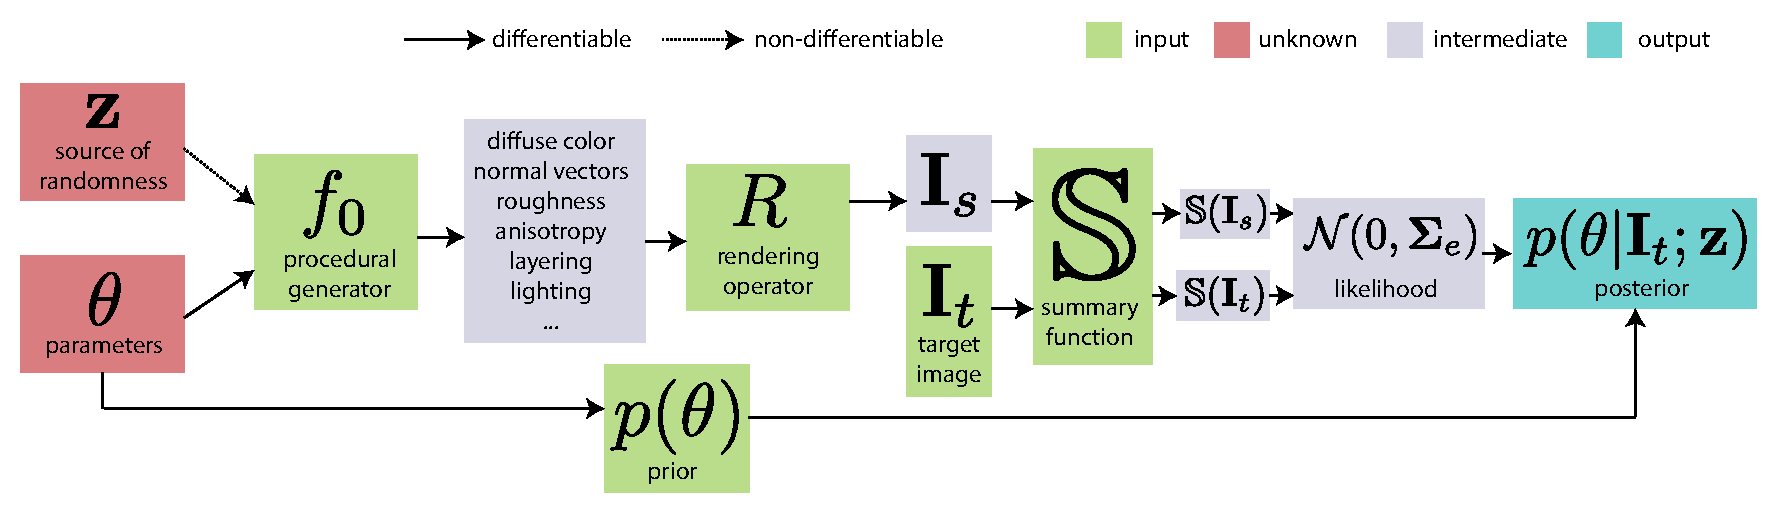
\includegraphics[width=\textwidth]{bayesian/fig1-2/posterior.pdf}
	\caption[Pipeline]{\label{fig:bayesian:pipeline}
		Our posterior computation combines priors, a procedural material model, a rendering operator, a summary function, and a target image. This posterior distribution can then be sampled to provide plausible values of the parameter vector. The value of the posterior is computed up to a normalization term, which does not effect MCMC sampling. The entire posterior definition is differentiable in the material parameters (excluding optional discrete model parameters).}
\end{figure}

Our second contribution is to introduce a \emph{Bayesian inference} approach capable of drawing samples from the space of plausible material parameters.
This provides additional information beyond single point estimates of material parameters (for example, though not limited to, discovering similarity structures in the parameter space).
Further, due to an ability to combine multiple Markov-Chain Monte Carlo (MCMC) sampling techniques such as Metropolis-Hasting (MH), Hamiltonian Monte Carlo (HMC), and Metropolis-adjusted Langevin algorithm (MALA), our technique is capable of efficiently handling both discrete and continuous model parameters.
Posterior sampling is a well-studied area within statistics and has been used in computer vision and inverse rendering \cite{Picture}, but to our knowledge, it has not yet been applied to material appearance acquisition.

To demonstrate the effectiveness of our framework, we fit procedural models for a diverse set of materials from standard opaque dielectrics (e.g. plastics, leather, wall paint) to dielectrics with 3D structure (wood) to anisotropic brushed metals and layered metallic paints (see Figure~\ref{fig:bayesian:teaser}, \S\ref{sec:bayesian:results}, and the supplemental materials).


\section{Related Work}
\label{sec:layeredbsdf:related}

\subsection{Discretized layered BSDFs}
Previously, a number of BSDF models have been proposed to describe layers with various assumptions on the interface and subsurface scattering.

An early analytical model by Hanrahan and Krueger \cite{hanrahan1993reflection} already supported multiple layers, but only single scattering, and without supporting arbitrary BSDFs at interfaces. They also proposed to add multiple scattering by Monte Carlo simulation, but their simulation approach only considers volume scattering events (as opposed to a combination of volume and rough interface events). Furthermore, it uses binning on the outgoing direction, as opposed to an efficient BSDF evaluation method for a given outgoing direction, which is provided by our approach.

A model by Stam \cite{stam2001illumination} introduces a solution for rendering skin as a layered material consisting of rough dielectric interfaces bounding a volumetric scattering slab. The solution is based on discretization of the BSDF into a directional basis, on which the light transport problem is solved. The model introduced by Jakob et al. \cite{jakob2014comprehensive} can be seen as a significant extension of Stam's discretization approach, working in the Fourier domain. It handles arbitrary layer stacks, supporting subsurface scattering within thin layers using the adding-doubling method, in addition to microfacet rough interfaces. The work of Zeltner extends this approach to anisotropic surface reflectance \cite{zeltner2018layer}. These models are highly accurate and efficient to render with, once the discretized BSDF has been constructed. However, as the BSDF construction in the discretized basis is relatively expensive, they are best suited for homogeneous BSDFs. A small number of such BSDFs can be spatially blended with varying weights, but this has strict limitations, compared to our support for arbitrary spatial texturing of all parameters.

\subsection{Analytic layered BSDFs}
The model by Weidlich and Wilkie \cite{weidlich2007arbitrarily} takes a different approach. They focus on layers where subsurface scattering is absent (though absorption is allowed), by analytically combining microfacet BSDFs from the interfaces into a single, potentially multi-lobe, microfacet-like BSDF. There are significant approximations in this approach, carefully chosen so that integration (Monte Carlo or otherwise) is never required within a single BSDF query. This makes the model fast and flexible. Another recent model \cite{guo2016rendering} also takes the approach of avoiding Monte Carlo integration during queries, by introducing extended normal distribution functions (ENDFs), analogous to microfacet NDFs but capturing multiple reflection or scattering events. In the most recent work, Belcour \cite{belcour2018efficient} introduced an approach based on tracking low-order moments of the BSDF lobes. This is a very fast and practical solution, but still introduces some approximations and limitations (e.g. no surface or volume anisotropy). In contrast, our method offers unbiased accuracy and even more flexibility, at the cost of some additional computation and variance. Several previous techniques model light scattering in layered materials like human skin~\cite{donner2008layered}, but these are focused on lateral light spreading in BSSRDFs, and are orthogonal to our focus on the directional properties of BSDF models.

\subsection{Microfacet models for interfaces}
BSDF models based on the microfacet theory are commonly used in computer graphics to capture how light reflects and refracts when interacting with specular surfaces with rough microstructure. The model by Walter et al. \cite{walter2007microfacet} extends the microfacet model of Cook and Torrance~\cite{cook1982reflectance} to handle light reflection and transmittance through rough dielectric interfaces, and is currently seen as standard in physically-based rendering. We use this model to describe our layer interfaces.

The microfacet model recently developed by Heitz et al.\cite{heitz2016multiple} is capable of capturing interreflections between the facets and better conserves energy. Sch\"ussler \cite{schussler2017microfacet} introduced a solution to the energy loss common in normal mapping techniques, caused by a mismatch between the shading and geometric normal. These models (or any future improved microfacet models) could be combined with our approach.

\subsection{Capability comparison}
\begin{figure}[h]
	\centering
	\setlength{\resLen}{1.2in}
	\addtolength{\tabcolsep}{-3.5pt}
	\begin{tabular}{ccc}
		\includegraphics[width=\resLen]{layeredbsdf/validations/compare2/aniso_comb_hor_hor_512spp_17min.jpg} &
		\includegraphics[width=\resLen]{layeredbsdf/validations/compare2/aniso_comb_hor_hor_wenzel.jpg} &
		\includegraphics[width=\resLen]{layeredbsdf/validations/compare2/na.pdf} \\		
		\includegraphics[width=\resLen]{layeredbsdf/validations/compare2/sphere_layered_1024spp_37min.jpg} &
		\includegraphics[width=\resLen]{layeredbsdf/validations/compare2/na2.pdf} &
		\includegraphics[width=\resLen]{layeredbsdf/validations/compare2/sphere_laurent_1024spp_1_5min.jpg} \\	
		\includegraphics[width=\resLen]{layeredbsdf/validations/compare2/sphere_1024spp_60min.jpg} &
		\includegraphics[width=\resLen]{layeredbsdf/validations/compare2/na.pdf} &
		\includegraphics[width=\resLen]{layeredbsdf/validations/compare2/na.pdf} \\
		Ours &
		Zeltner 2018 \cite{zeltner2018layer} &
		Belcour 2018 \cite{belcour2018efficient}
	\end{tabular}
	\caption[Comparison to previous work]{\label{fig:layeredbsdf:compare_previous}
		\textbf{Comparison to previous work.} The \textbf{top row} shows an example with anisotropic surface reflectance, where our solution closely matches Zeltner's, but Belcour's approach does not support anisotropy. The \textbf{middle row} shows an example with spatial variation in the parameters; here our method closely matches Belcour's, but Zeltner's approach does not naturally support spatial variation. The \textbf{bottom row} shows a two-layer configuration with anisotropic microflake phase functions, which is only supported by our method.
	}
\end{figure}

In Figure \ref{fig:layeredbsdf:compare_previous}, we compare the capabilities of our approach to recent work \cite{zeltner2018layer,belcour2018efficient}. We consider three features supported by our approach: surface anisotropy, spatial variation, and volumetric medium anisotropy. Only one of these is supported in the compared systems: spatial variation in Belcour's approach and surface anisotropy in Zeltner's.


%\chapter{Background}
\label{cpt:background}

In this chapter, we briefly review some background knowledge closely related to this dissertation. Firstly, we recap the fundamental light transport theory and Bidirectional Reflectance Distribution Function (BRDF). Then we introduce Maxwells' equation in wave optics. Finally we talk about some concepts in Markov Chain Monte Carlo (MCMC) methods. 

\section{Light Transport}
Radiometry is a set of techniques for measuring electromagnetic radiation, and we use is to measure the energy of visible lights in nowadays renderings. First we list some important Radiometric quantities and then describe rendering equations in the following sections.

\begin{table}[!ht]
	\centering
	\caption[List of radiometry quantities]{\label{tab:background:notation}
		List of radiometry quantities.
	}
	\begin{tabular}{cccc}
		Quantity & Symbol & Unit & Notes \\
		\hline
		\multirow{2}{*}{Flux(Power)} & \multirow{2}{*}{$\Phi$} & \multirow{2}{*}{W} & Radiant energy emitted, reflected, \\
		 & & & transmitted or received, per unit time. \\[0.2em]
		Irradiance & $E$ & $W/m^2$ & Flux received by a surface per unit area. \\[0.2em]
		Radiance & $L$ & $W/(Sr\cdot m^2)$ $^*$ & Flux per unit solid angle per unit projected area. \\
		\hline
		\multicolumn{3}{l}{\footnotesize{$^*$ watt per steradian per square meter.}}	
	\end{tabular}
\end{table}

\subsection{Surface rendering equation}
To render photorealistic image, a key concept is to simulate light transport, which models the light interaction between camera/eyes, scene objects and lightsource. For any point in the scene, we want to know its spectral radiance $\Lo(\bmr,\bmomegao,\lambda,t)$ of wavelength $\lambda$ directed outward along direction $\bmomegao$ at time $t$, from a particular position $\bmr$. For simplisity, the commonly used \emph{rendering equation} (RE) \cite{kajiya1986rendering} for surface have two assumptions: geometric optics only and steady state. Therefore, we reformulate the light radiance as a $5D$ function of position ($\bmr$) and direction ($\bmomegao$), the outgoing radiance ($\Lo$) is the sum of the emitted radiance ($\Le$) and the reflected radiance ($\Lr$). The reflected radiance itself is the sum of all directions of incoming radiance ($\Li$) weighted by the surface reflection ($\fr$) and cosine of incident angle.
\begin{equation}     	
	\begin{aligned}
		\Lo(\bmr,\bmomegao) &= \Le(\bmr,\bmomegao) + \Lr(\bmr,\bmomegao) \\
		&= \Le(\bmr,\bmomegao) + 
		\int_{\bbSS} \Li(\bmr,\bmomegai) \fr(\bmr,\bmomegai\rightarrow\bmomegao) \EV{\bmn(\bmr),\bmomegai} \intd \bmomegai
	\end{aligned}
\end{equation}
Note that, $\bmomegao$ is the direction of the outgoing light, and $\bmomegai$ is the negative direction of the incoming light. 

The rendering equation can fully model the light transport in a space without any participating media. It is popular to expand this integral equation to \emph{path integral formulation} and solve it using Monte Carlo methods (see Veach's thesis 
\cite{veach1997metropolis}).


\subsection{Volume rendering equation}
When light travels in a participation medium (e.g., smoke, marble and skin), we use \emph{radiative transfer equation} (RTE) \cite{chandrasekhar1960radiative} to describe how the radiance changes by four types of interaction events: emission, absorption, out-scattering, and in-scattering.
\begin{equation}
	\begin{aligned}
		(\bmomegao\cdot\nabla) \Lo(\bmr,\bmomegao) &= 
		\overbrace{\sigmas(\bmr,\bmomegao) \int_{\bbSS} \Li(\bmr,\bmomegai)\fp(\bmr,\bmomegai\rightarrow\bmomegao) \intd\bmomegai}^{\text{a) In-scattering}} \\
		& \overbrace{-\sigmas(\bmr,\bmomegao)\Lo(\bmr,\bmomegao)}^{\text{b) Out-scattering}}
		\overbrace{-\sigmaa(\bmr,\bmomegao)\Lo(\bmr,\bmomegao)}^{\mathrm{c) Absorption}}
		\overbrace{+\Le(\bmr,\bmomegao)}^{\mathrm{d) Emission}}
	\end{aligned}
\end{equation}
The RTE is a integro-differential equation which can be derived via conservation of energy. Briefly, the RTE states that a beam of light loses energy through divergence and extinction (including both absorption (c) and scattering (b) away from the beam) and gains energy from light sources (d) in the medium and scattering (a) directed towards the beam. Same as RE, coherence, polarization and light speed are neglected. Optical properties such as refractive index ($m$), absorption coefficient ($\sigmaa$), scattering coefficient ($\sigmas$) are taken as time-invariant but may vary spatially. In addition, we define the extinction coefficient $\sigmat = \sigmaa + \sigmas$, and the ratio between $\sigmas$ and $\sigmat$ controls the fraction of radiant energy not being absorbed at each scattering and is also known as the single-scattering albedo ($a$). We use phase functions $\fp(\bmomegai\rightarrow\bmomegao)$ to describe the directional distribution of light scattered in a medium.

It is desirable to rewrite the RTE as an integral equation, which can them be solved numerically using Monte Carlo methods (see Veach's thesis 
\cite{veach1997metropolis}). 

\section{Scattering Distribution Function}
In RE and RTE, an important term is still missing. When light hit a surface or a particle in the medium, how does the light scatter, or in other words, redistribute both in energy and direction? To model this scattering effect, we use \emph{bidirectional reflectance distribution function} (BRDF) for surface interaction and \emph{phase function} (PF) for light scattering in a medium.

\subsection{Bidirectional reflectance distribution function (BRDF)}
The BRDF is a 4-$D$ function that defines how light is reflected at an opaque surface. 
\begin{equation}
	\fr(\bmomegai\rightarrow\bmomegao) = \frac{\intd \Lo(\bmomegao)}{\intd \Ei(\bmomegai)}
	= \frac{\intd\Lo(\bmomegao)}{\Li(\bmomegai)\EV{\bmn,\bmomegai}\intd\bmomegai}
\end{equation}
The function takes an incoming light direction $\bmomegai$, and outgoing direction $\bmomegao$, and returns the ratio of reflected radiance ($\Lo$) exiting along $\bmomegao$ to the irradiance incident ($\Li$) on the surface from direction $\bmomegai$. Each direction $\bmomega$ is itself parameterized by azimuth angle $\varphi$ and polar angle $\theta$. $\bmn$ is the (macro) surface normal.

Physically based BRDFs have several properties, including,

Positivity: 
\begin{equation}
	\fr(\bmomegai\rightarrow\bmomegao) \geq 0
\end{equation}
Reciprocity:
\begin{equation}
	\fr(\bmomegai\rightarrow\bmomegao) = \fr(\bmomegao\rightarrow\bmomegai)
\end{equation}
Conserving energy:
\begin{equation}
	\forall\bmomegao, \int_{\bbSS} \fr(\bmomegai\rightarrow\bmomegao) \EV{\bmn,\bmomegai} \leq 1
\end{equation}

Some basic BRDFs and the BRDFs used in this dissertation are listed below:

\paragraph{Lambertian BRDF} distribute the incident energy equally towards all the outgoing directions and give a diffuse appearance.
\begin{equation}
	\fr(\bmomegai\rightarrow\bmomegao) = \kd
\end{equation}
where $\kd$ is the albedo or absorption of light which will introducing the color.

\paragraph{Phong and Blinn-Phong BRDF} adds a specular component to introduce glossy effect.
\begin{equation}
	\fr(\bmomegai\rightarrow\bmomegao) = \kd + \ks({\bmomegai}_\mathrm{r} \cdot \bmomegao)^n
\end{equation}
where ${\bmomegai}_\mathrm{r}$ is the reflection of incident light and larger $n$ will increase the glossiness of the material. 

\paragraph{Microfacet BRDF} is the state-of-the-art model which is widely used in all kinds of renderers. The microfacet theory assumes that all surfaces are formed by tiny microfacets that are perfectly specular that reflect rays like perfectly smooth mirrors.
\begin{equation}
	\fr(\bmomegai\rightarrow\bmomegao) = 
	\frac{F(\bmomegai, \bmh) G(\bmomegai,\bmomegao,\bmh) D(\bmh)}
	{4\EV{\bmn,\bmomegai}\EV{\bmn,\bmomegao}}
\end{equation}
where $\bmh$ is the half vector that $\bmh=(\bmomegai+\bmomegao)/2$. The first component $F$ is Fresnel term, $G$ is the geometry term (shading factor) and $D$ is \emph{normal distribution function} (NDF) which indicate the distribution of microfacets normals. With the change of statistics of the micro-geometry, the macro-properties changes accordingly.
All NDF should follow:
\begin{equation}
	\int_{\bbSS} D(\bmh)\EV{\bmn,\bmh} \intd\bmh = 1
\end{equation}
There're two forms of NDF we used in most of the papers, \emph{Beckmann} and \emph{GGX}.

BRDF is a special case for opaque surface with reflection only. It can be extend to \emph{bidirectional transmittance distribution function} (BTDF) for  opposite side of the surface, and \emph{bidirectional scattering distribution function} (BSDF), a superset and generalization of BRDF and BTDF.

%\emph{Beckmann}:
%\begin{equation}
%	D(\bmh) = \frac{1}{\pi\alpha^2\cos^4\theta}\Exp^{-\frac{\tan^2\theta}{\alpha^2}}
%\end{equation}
%
%\emph{GGX}:
%\begin{equation}
%	D(\bmh) = \frac{\alpha^2}{\pi((\alpha^2-1)\cos^2\theta+1)^2}
%\end{equation}


\paragraph{Spatially varying BRDF}
The \emph{spatially varying BRDF} (SVBRDF) is a 6-$D$ function, $\fr(\bmr,\bmomegai,\bmomegao)$, where $\bmr$ describes a 2D location over an object's surface.


\subsection{Phase function}
Phase function is usually parameterized as a function of the angle ($\theta$) between $\bmomegai$ and $\bmomegao$, to model how light scattered in medium. A common phase function is \emph{Henyey-Greenstain} (HG) phase function with parameter $-1<g<1$:
\begin{equation}
	\fp(\theta,g) = \frac{1}{4\pi}
	\frac{1-g^2}
	{(1+g^2-2g\cos\theta)^{3/2}}
\end{equation}


\section{Maxwell Equations}

\subsection{Basic operators and notation}

The differential operator given in Cartesian coordinates $\{x,y,z\}$: 
\begin{equation}
	\nabla = \frac{\partial}{\partial x}\mathbf{i} + \frac{\partial}{\partial y}\mathbf{j} + \frac{\partial}{\partial z}\mathbf{k}
\end{equation}
For a scalar function $f(x,y,z)$ and a vector field $\bfF(x,y,z) = f_1(x,y,z)\mathbf{i} + f_2(x,y,z)\mathbf{j} + f_3(x,y,z)\mathbf{k}$, we have,

Gradient:
\begin{equation}
	\nabla f = \frac{\partial f}{\partial x}\mathbf{i} + \frac{\partial f}{\partial y}\mathbf{j} + \frac{\partial f}{\partial z}\mathbf{k}
\end{equation}
Divergence: 
\begin{equation}
	\Div\bfF = \frac{\partial f_1}{\partial x} + \frac{\partial f_2}{\partial y} + \frac{\partial f_3}{\partial z}
\end{equation}
Curl: 
\begin{equation}
	\Curl\bfF = \left|
	\begin{array}{ccc}
		\mathbf{i} & \mathbf{j} & \mathbf{k} \\
		\frac{\partial}{\partial x} & \frac{\partial}{\partial y} & \frac{\partial}{\partial z} \\
		f_1 & f_2 & f_3
	\end{array}
	\right|
\end{equation}	
Laplace operator: $\nabla^2 f = \Div(\nabla f)$

Curl of Curl: 
	$\Curl(\Curl\bfF) = \nabla(\Div\bfF) - \Div(\nabla\bfF) = - \Div(\nabla\bfF) = -\nabla^2\bfF$


\subsection{Derivation}

\begin{table}[!ht]
	\centering
	\caption[List of Maxwell notations]{\label{tab:background:notation2}
		List of Maxwell notations.
	}
	\begin{tabular}{ccl}
		Symbol & Unit & Notes \\
		\hline
		$\bfE$ & $V/m$      & Electric field \\
		$\bfH$ & $A/m$      & Magnetic field \\
		$\bfD$ & $C/m^2$    & Electric displacement \\
		$\bfB$ & $Wb/m^2$   & Magnetic induction \\
		$\bfJ$ & $A/m^2$    & Electric current density \\
		$\bfM$ &            & Magnetic current density \\
		$\bfP$ &            & Electric polarization \\
		$\rho$ & $C/m^3$    & Electric charge density \\
		$q$    & $Wb/m^3$   & Magnetic charge density \\
		$\varepsilon_0$     & $F/m$ & Electric permittivity of free space ($=8.854187817\times10^{-12}$) \\
		$\mu_0$             & $H/m$ & Magnetic permeability of free space ($=4\pi\times10^{-7}$) \\
	\end{tabular}
\end{table}

The mathematical description of Maxwell’s equations are \cite{bohren2008absorption}:
\begin{equation}
	\begin{aligned}
		\Div\bfD  &= \rho & & & & & \Div\bfB &= 0 \\
		\Curl\bfE &= -\frac{\partial\bfB}{\partial t} & & & & & 
		\Curl\bfH &= \mathbf{J} + \frac{\partial\bfD}{\partial t}
  \end{aligned}
\end{equation}
where, $\bfD = \varepsilon_0\bfE + \bfP$ and 
	$\bfH = \frac{1}{\mu_0}\bfB - \bfM$.

In free space, the polarization ($\bfP$) and magnetization ($\bfM$) vanish identically. And if there is no Electric charge density ($\rho$) and Electric current density ($\mathbf{J}$), we rewrite \textit{Maxwell equation} in the form of $\bfE$ and $\bfH$,
\begin{equation}
	\begin{aligned}
		\Div\bfE  &= 0 & & & & & \Div\bfH  &= 0 \\
		\Curl\bfE &= -\mu_0\frac{\partial\bfH}{\partial t} & & & & & 
		\Curl\bfH &= \varepsilon_0\frac{\partial\bfE}{\partial t}
  	\end{aligned}
\end{equation}
To consider Electric and Magnetic field as as time-harmonic (time variation is sinusoidal) fields with angular frequency of $\omega$, which has the form of $\mathbf{\hat{u}} = \mathbf{u}e^{-i\omega t}$, the \textit{Maxwell equation} become,
\begin{equation}
	\begin{aligned}
		\Div\bfE  &= 0 & & & & & \Div\bfH  &= 0 \\
		\Curl\bfE &= i\omega\mu_0\bfH & & & & & 
		\Curl\bfH &= -i\omega\varepsilon_0\bfE \label{eq:nabla}
	\end{aligned}
\end{equation}
Take the curl of (\ref{eq:nabla}), 
\begin{equation}
	\begin{aligned}
		\Curl(\Curl\bfE) &= i\omega\mu_0(\Curl\bfH) = \omega^2\mu_0\varepsilon_0\bfE \\
		\Curl(\Curl\bfH) &= -i\omega\varepsilon_0(\Curl\bfE) = \omega^2\mu_0\varepsilon_0\bfH
	\end{aligned}
\end{equation}
If we use the rule \emph{Curl of Curl}, the \textit{Maxwell equations} reduce to the Helmholtz equations,
\begin{equation}
	\begin{aligned}
		\nabla^2\bfE + k^2\bfE = 0 & & & & & 
		\nabla^2\bfH + k^2\bfH = 0
	\end{aligned}
\end{equation}
where $k = \omega/c$, and $c=\frac{1}{\sqrt{\mu_0\varepsilon_0}}$ is the light speed in vacuum. 


\section{Bayesian Inference}
Bayesian inference is a paradigm for constructing statistical models based on Bayes’ Theorem
\begin{equation}
	p(\bmtheta|\bfX) = \frac{p(\bfX|\bmtheta)p(\bmtheta)}{p(\bfX)} \propto p(\bfX|\bmtheta)p(\bmtheta)
\end{equation}
Generally speaking, the goal of Bayesian inference is to estimate the posterior distribution ($p(\bmtheta|\bfX)$) given the likelihood ($p(\bfX|\bmtheta)$) and the prior distribution ($p(\bmtheta)$). The likelihood is something that can be estimated from the training data. 

\subsection{Maximum a Posteriori (MAP)}
In most of cases, we actually seek to maximize the posterior distribution which takes the existing data as fixed and determines the probability of any parameter setting $\bmtheta$ given that data $\bfX$. We call this process \emph{Maximum a Posteriori} (MAP), an iterative process which updates the model’s parameters in an attempt to maximize the probability of matching data to its distribution. Which is exactly the training pocess in a regular machine learning model.

MAP estimates can be computed via numerical optimization such as the conjugate gradient method or Newton's method. This usually requires first or second derivatives, which have to be evaluated analytically or numerically.

\subsection{Markov Chain Monte Carlo (MCMC)}
While MAP is the first step towards fully Bayesian inference, it’s still only computing what statisticians called a \emph{point estimate}. The downside of point estimates is that they don’t tell you much about a parameter other than its optimal setting. In reality, we often want to know other information, like how certain we are that a parameter’s value should fall within this predefined range. Therefore, a number of fascinating Bayesian methods have been devised that can be used to sample (i.e. draw sample values) from the posterior distribution. The most famous of these is an algorithm called \emph{Markov Chain Monte Carlo} (MCMC).

In statistics, MCMC methods comprise a class of algorithms for sampling from a probability distribution. By constructing a Markov chain that has the desired distribution as its equilibrium distribution, one can obtain a sample of the desired distribution by recording states from the chain. The more steps are included, the more closely the distribution of the sample matches the actual desired distribution. 

MCMC is used to simulate physical systems with Gibbs canonical distribution (\textbf{we will start to use $\bfx$ instead of $\bmtheta$ from here}):
\begin{equation}
	p(\bfx) \propto \exp\left( - \frac{U(\bfx)}{T} \right)
\end{equation}
Probability $p(\bfx)$ of a system to be in the state $\bfx$ depends on the energy of the state $U(\bfx)$ and temperature $T$.
Any distribution can be rewritten as Gibbs canonical distribution, but for many problems such energy-based distributions appear very naturally.
The goal becomes learning to sample from the canonical distribution.
System has higher probability of staying in the states with lower energies, so minimize energy is the same as maximum a posteriori.

\paragraph{Metropolis-Hastings (MH)} algorithm for MCMC is the simplest Markov Chain process that can sample from the distribution picks the neighbour of the current state and either accepts it or rejects depending on the change in energy. 
Algorithm produces a chain of states: $ \bfx_1, \bfx_2, ..., \bfx_n $. Each time a candidate from a neighborhood of the last state is selected
$\bfx_n' = \bfx_n + \varepsilon$ ($\epsilon$ is usually taken to be Gaussian with some spread $\sigma$).
With probability $p = \min \left[1, \exp\left( \frac{U(\bfx_n) - U(\bfx_n')}{T} \right) \right]$, system accepts new state (jumps to the new state):
$\bfx_{n+1} = \bfx_n'$ and with probability $1-p$ new state is rejected: $\bfx_{n+1} = \bfx_n$.
Note, when energy is lower in new state $U(\bfx'_n) < U(\bfx_n)$, it is always accepted: $p=1$.
In this way, we give preference to the states with lower energies, while not restricting the algorithm to always decrease the energy.
The lower temperature, the lower probability to increase energy.

Sampling high-dimensional distributions with MH becomes very inefficient in practice. A more efficient scheme is

\paragraph{Hamiltonian Monte Carlo (HMC)} algorithm, is also known as Hybrid Monte Carlo. Velocity $v$ is added to the parameters describing the system. Energy of the system consists of potential and kinetic parts:	$E(\bfx, \bfv) = U(\bfx) + K(\bfv)$. %$\qquad K(\bfv) = \sum_i \frac{m \, v^2_i}{2}$. 
Thus, velocities $\bfv$ and positions $\bfx$ have independent canonical distributions:
\begin{equation}
	p(\bfx, \bfv) \propto \exp\left(  \frac{-E(\bfx, \bfv)}{T}  \right)
	= \exp\left(  \frac{-U(\bfx)}{T}  \right) \, \exp \left( \frac{-K(\bfv)}{T} \right) \propto p(\bfx) \; p(\bfv).
\end{equation}
So once it can be sampled from joint distribution $p(\bfx, \bfv)$, $\bfx$ can be also sampled by ignoring computed velocities $\bfv$.
After initializing the system parameters $\bfx, \bfv$, it could be evolved using physics equations: $\dot{x}_i = v_i$, $m\dot{v_i} = -\frac{\partial U(\bfx)}{\partial x_i}$. During a long period of time, it will not get a canonical distribution by collecting system states, because energy $E$ is conserved in the system.
At some points, velocity is resampled from $p(\bfv)$, thus changing the total energy and resample the parameters. Sampling from $p(\bfv)$ is very simple, because $\bfv$ is normally distributed.

HMC uses not only energy $U(\bfx)$, but also it's gradient. So the `price' of a single iteration is higher, but HMC is still significantly more efficient than MH.
In most cases HMC accepts new states, but still, it has problems with sampling from distributions with isolated local minimum and discrete parameters (no gradient provided).

\paragraph{Metropolis-Adjusted Langevin Algorithm (MALA)} is based on \emph{Langevin Monte Carlo} (LMC). Different from gradient-based HMC, LMC uses a discrete Markov chain, which is equivalent to a gradient ascent procedure with injected Gaussian noise \cite{luan2020langevin}. The injected noise prevents the chain from collapsing to just the (local) maximum. Due to discretization error, the Markov chain is not guaranteed to converge to the same stationary distribution as the continuous process.
This can be corrected by using the Metropolis-Hasting rule to accept or reject states of the chain. This approach, known as the \emph{Metropolis-adjusted
Langevin algorithm} (MALA).

%\section{Notation}
%\begin{table}[h]
    \centering
    \addtolength{\tabcolsep}{-2pt}
    \small    
    \begin{tabular}{cccc|cccccc}
         & \textbackslash bm &  \textbackslash mathrm & \textbackslash mathbf & 
         & \textbackslash bm &  \textbackslash mathrm & \textbackslash mathbf & \textbackslash mathbb & \textbackslash mathcal \\
        \hline
        $a$ & $\bm{a}$ & $\mathrm{a}$ & $\mathbf{a}$ &  
        $A$ & $\bm{A}$ & $\mathrm{A}$ & $\mathbf{A}$ & $\mathbb{A}$ & $\mathcal{A}$ \\
        $g$ & $\bm{g}$ & $\mathrm{g}$ & $\mathbf{g}$ &  
        $G$ & $\bm{G}$ & $\mathrm{G}$ & $\mathbf{G}$ & $\mathbb{G}$ & $\mathcal{G}$ \\
        $q$ & $\bm{q}$ & $\mathrm{q}$ & $\mathbf{q}$ & 
        $Q$ & $\bm{Q}$ & $\mathrm{Q}$ & $\mathbf{Q}$ & $\mathbb{Q}$ & $\mathcal{Q}$ \\
        $x$ & $\bm{x}$ & $\mathrm{x}$ & $\mathbf{x}$ & 
        $X$ & $\bm{X}$ & $\mathrm{X}$ & $\mathbf{X}$ & $\mathbb{X}$ & $\mathcal{X}$ \\
        $y$ & $\bm{y}$ & $\mathrm{y}$ & $\mathbf{y}$ & 
        $Y$ & $\bm{Y}$ & $\mathrm{Y}$ & $\mathbf{Y}$ & $\mathbb{Y}$ & $\mathcal{Y}$ \\
        $z$ & $\bm{z}$ & $\mathrm{z}$ & $\mathbf{z}$ & 
        $Z$ & $\bm{Z}$ & $\mathrm{Z}$ & $\mathbf{Z}$ & $\mathbb{Z}$ & $\mathcal{Z}$ \\        
        \hline
		$\sigma$ & $\bm{\sigma}$ & $\mathrm{int}$ & $\text{int}$ &
		$\Sigma$ & $\bm{\Sigma}$ & & & & \\
		$\delta$ & $\bm{\delta}$ & $\mathbf{int}$ & $\textbf{int}$ & 
		$\Delta$ & $\bm{\Delta}$ & & & & \\
		$\theta$ & $\bm{\theta}$ & $int$ & $\bm{int}$ & 
		$\Theta$ & $\bm{\Theta}$ & & & & \\
		$\phi$ & $\bm{\phi}$ & & & 
		$\Phi$ & $\bm{\Phi}$ & & & & \\
    \end{tabular}
\end{table}




%\input{tex/layeredbsdf/path-formulation}
%\input{tex/layeredbsdf/ours}
%\input{tex/layeredbsdf/result}
%\chapter{Conclusion and Future work}
\label{cpt:conclusion}

In the dissertation, we focus on material appearances modeling in both forward and inverse rendering. All the macro appearances are modeled from microscales or hyperparameter spaces. 

First we have presented two scattering frameworks in forward rendering, one for layered materials (\emph{thin planer surface}) and the other one for participating medium (\emph{bulk,particles}). The first work \textbf{LayeredBSDF} provides a general solution to layered materials which is included in \emph{Physically Based Rendering}, Fourth Edition \cite{pharr2021physically}. It leads to the first BSDF layering solution that offers unbiased accuracy and full flexibility in setting the layer properties.
Our second work \textbf{Beyond Mie Theory} generalizes the widely-used Lorenz-Mie theory for rigorously deriving optical properties of scattering media, and can be readily used in any radiative-based light transport simulator.

Then we have estimated material properties using \emph{latent space} and \emph{procedural parameters}. Our third work \textbf{MaterialGAN} is the first step toward GAN-based material analysis and synthesis and our experiments suggest many avenues for further exploration. Our last work \textbf{Bayesian Inference Sampling} handles both continuous and discrete model parameters and provides users additional information beyond single point estimates and allows a
cleaner extension to handle discrete parameters.

At the end, we will discuss the limitation of our work and future directions:

\paragraph{LayeredBSDF}
Our model relies on the assumption of thin flat layers (Figure \ref{fig:layeredbsdf:zhaoyun}) and cannot capture effects caused by geometric or optical variations at the global scale.
Examples include internal caustics and shadowing arising from major normal variations and color bleeding caused by light scattering though media with varying colors.
Generalizing our technique to include bidirectional subsurface scattering distribution functions (BSSRDFs) is an interesting further topic.
In addition, as our model simulates subsurface scattering using Monte Carlo path tracing, the performance may degrade with the presence of optically thick layers with many scattering events.
Using fast approximated solutions such as \cite{jensen2001practical,frisvad2014directional} to capture multiple scattering may be a useful extension.
Lastly, since we model light transport using traditional radiative transfer, wave effects such as thin film interference are not handled.
An interesting challenge is to integrate wave optics into our model to accurately and efficiently handle light interference and phase shifts.

\paragraph{Beyond Mie Theory}
While taking into account the effect of the near-field on clusters, our work is still based on the RTT. Therefore it relies on the far-field approximation to represent a scattering dyad useful for rendering. Therefore, while we can handle near- and far-field scattering, we cannot accurately model the scattering in the intermediate region, which we treat as the far field. Using more accurate representations, that capture the effects at such near-field region could further enhance the generality of our theory and, thus, is an interesting future topic. This would however require exploring an alternative light transport framework beyond the RTT.
Right now, our implementation requires precomputing the bulk optical properties of the media. This limits the applicability of our work to media with homogeneous particle statistical properties. Finding faster approximations for our scattering functions, in the same spirit as the geometric optics approximation for Lorenz-Mie theory \cite{glantschnig1981light}, is an interesting future research. 
Finally, our implementation is currently limited in practice to spherical particles with identical radii within a particle cluster. Allowing general and spatially varying particle shapes by using an alternative implementation of the T-matrix method would further improve the versatility of our technique.

\paragraph{MaterialGAN}
Our current BRDF model is shared by previous work, but certain common effects (layering on book covers, subsurface fiber scattering in woods, anisotropy in fabrics) are not correctly captured by it. An extension of our generative model and rendering operator would be possible, though the key challenge is finding high-quality  training data for these effects.
Our assumption of almost flat samples will fail for materials with strong relief patterns, and will produce blurring or ghosting if there are obvious parallax effects in the aligned captured images. Strong self-shadowing or inter-reflections are also not currently handled. Solving for height instead of normal, with a more advanced rendering operator, may be able to resolve parallax effects and to correctly predict (and undo) shadowing effects from strong height variations.
Furthermore, more precise calibration may improve our accuracy. This would likely require knowledge of the cell phone hardware, and/or pre-calibration of its properties (e.g. flash light falloff, lens vignetting, and color processing properties).
The resolution of our result can be increased with a coarse-to-fine post-process, since we have a fairly good result as the initialization of next level of resolution.

\paragraph{Bayesian Inference Sampling}
In the future, we would like to increase the complexity of the models supported even further, to handle materials like woven fabrics, transmissive BTDFs, and more. Finally, extensions to our approach could be used to estimate parameters of procedural models beyond materials, including geometry and lighting, as long as the parameters could be differentiated.



\chapter{Microscale Based Volumetric Rendering}
\label{cpt:waveoptics}

\begin{figure}[!ht]
    \centering
    \setlength{\resLen}{1.02in}
    \addtolength{\tabcolsep}{-4pt}
    \small
    \begin{tabular}{cccccc}
        \includegraphics[height=\resLen]{waveoptics/slab/N1_300nm.jpg} &
        \includegraphics[height=\resLen]{waveoptics/slab/N100_300nm.jpg} &
        \includegraphics[height=\resLen]{waveoptics/slab/N100_500nm.jpg} &
        \includegraphics[height=\resLen]{waveoptics/slab/color.jpg} & 
        \includegraphics[height=\resLen]{waveoptics/slab/aniso_y.jpg} &
        \includegraphics[height=\resLen]{waveoptics/slab/pos.jpg}
        \\
        \includegraphics[height=\resLen]{waveoptics/particle/300nm_N1.jpg} &
        \includegraphics[height=\resLen]{waveoptics/particle/300nm_N100.jpg} &
        \includegraphics[height=\resLen]{waveoptics/particle/500nm_N100.jpg} &
        \includegraphics[height=\resLen]{waveoptics/particle/500nm_N100.jpg} &
        \includegraphics[height=\resLen]{waveoptics/particle/aniso.jpg} &
        \includegraphics[height=\resLen]{waveoptics/particle/pos.jpg}
        \\
        $\Ncls=1$   &
        $\Ncls=100$ &
        $\Ncls=100$ &
        $\Ncls=100$ & 
        $\Ncls=100$ &
        $\Ncls=100$
        \\
        $a_i=300\text{nm}$ &
		$a_i=300\text{nm}$ &
		$a_i=500\text{nm}$ &
		$a_i=500\text{nm}$ & 
		$a_i=500\text{nm}$ &
		$a_i=500\text{nm}$
		\\
        Isotropic & Isotropic & Isotropic & Isotropic & Anisotropic & Pos. correlated
        \\
        $\lambda=700\text{nm}$ &
        $\lambda=700\text{nm}$ &
        $\lambda=700\text{nm}$ &
        Multi-spectral &
        $\lambda=700\text{nm}$ &
        $\lambda=400\text{nm}$
    \end{tabular}
    \caption[Teaser]{\label{fig:waveoptics:teaser}
        We introduce a new technique to compute bulk scattering parameters (i.e., the extinction and scattering coefficients as well as the single-scattering phase function) in a systematic fashion. By considering wave optical effects and particle (scatterer) interactions at the microscopic level, our technique enjoys the generality of supporting a wide range of media (e.g., isotropic, anisotropic, and correlated).
        In this figure, we show renderings of thin slabs lit with a small area light from behind (top).
        Additionally, we show visualizations of the corresponding particle distributions (middle) as well as per-cluster particle counts~$\Ncls$ radii $a_i$ (bottom).
    }
\end{figure}

\section{Introduction}
\label{sec:bayesian:intro}

Physically accurate simulation of material appearance is an important yet challenging problem, with applications in areas from entertainment to product design and architecture visualization.
A key ingredient to photorealistic rendering is high-quality material appearance data.
Acquiring such data from physical measurements such as photographs has been an active research topic in computer vision and graphics. Recently, \emph{procedural} material models have been gaining significant traction in the industry (e.g., Substance \cite{Substance}).
In contrast to traditional texture-based spatially varying BRDFs that represent the variation of surface albedo, roughness, and normal vectors as 2D images, procedural models generate such information using a smaller number of user-facing parameters, providing high compactness, easy editability, and automatic seamless tiling.

The estimation of procedural model parameters faces several challenges. First, the procedural generation and physics-based rendering of materials is a complex process with a diverse set of operations, making the relationship between procedural model parameters and properties of the final renderings non-linear and non-trivial.
Additionally, designing a suitable loss function (metric) to compare a synthesized image to a target image is not obvious. Finally, given the soft nature of the image matching problem, a single point estimate of the ``best'' match may be less informative than a collection of plausible matches that a user can choose from.

In this paper, we introduce a new computational framework to estimate the parameters of procedural material models that focuses on these issues.
Our framework enjoys high generality by not requiring the procedural model to take any specific form, and supporting any differentiable BRDF models, including anisotropy and layering.

To design the loss function, we consider neural summary functions (embeddings) based on Gram matrices of VGG feature maps \cite{Gatys2015,Gatys2016}, as well as hand-crafted summary functions~(\S\ref{sec:summary_func}). The VGG feature map approach is becoming standard practice in computer vision, and was first introduced to material capture by Aittala et al. \cite{Aittala2016}; we extend this approach to procedural material estimation.

We make two main contributions. The first contribution is a unified view of the procedural parameter estimation problem in a \emph{Bayesian framework}~(\S\ref{sec:bayesian:bayesian}), precisely defining the posterior distribution of the parameters given the captured data and priors, allowing for both maximization and sampling of the posterior. Four components (priors, procedural material model, rendering operator, summary function) together define our posterior distribution (outlined in Figure \ref{fig:bayesian:pipeline}). 

\begin{figure}[!ht]
	\centering
	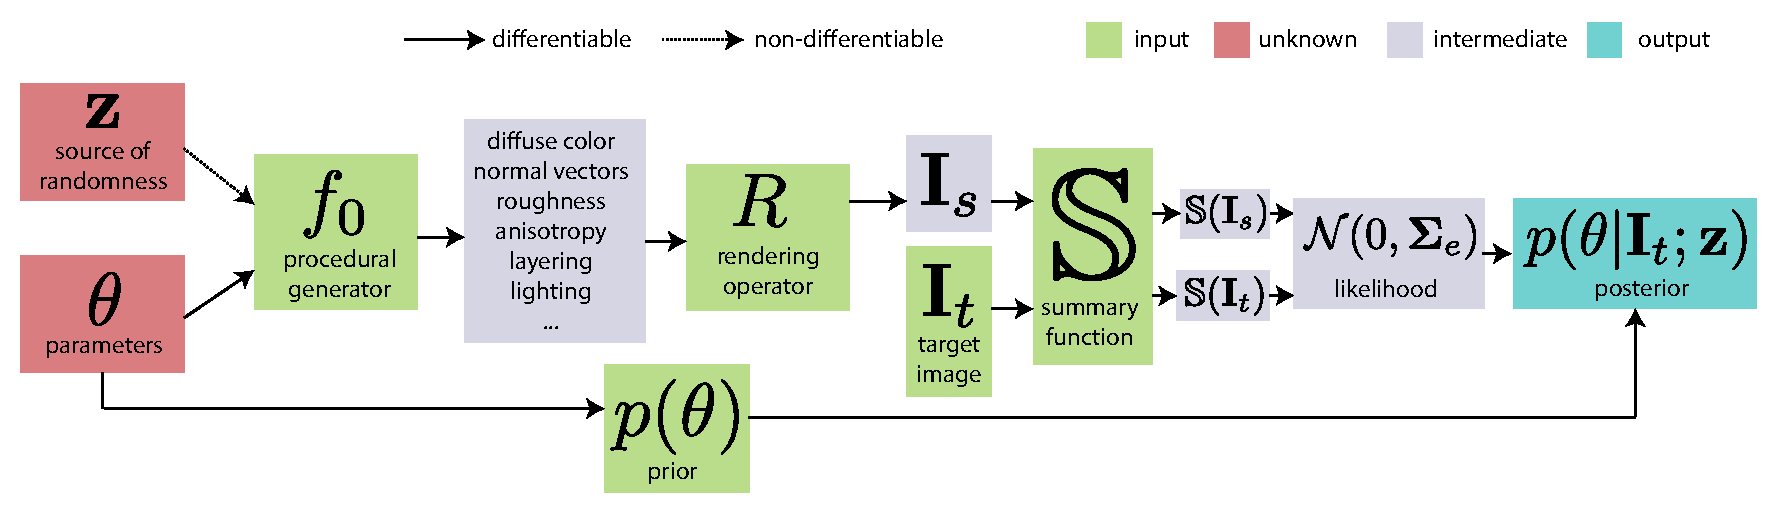
\includegraphics[width=\textwidth]{bayesian/fig1-2/posterior.pdf}
	\caption[Pipeline]{\label{fig:bayesian:pipeline}
		Our posterior computation combines priors, a procedural material model, a rendering operator, a summary function, and a target image. This posterior distribution can then be sampled to provide plausible values of the parameter vector. The value of the posterior is computed up to a normalization term, which does not effect MCMC sampling. The entire posterior definition is differentiable in the material parameters (excluding optional discrete model parameters).}
\end{figure}

Our second contribution is to introduce a \emph{Bayesian inference} approach capable of drawing samples from the space of plausible material parameters.
This provides additional information beyond single point estimates of material parameters (for example, though not limited to, discovering similarity structures in the parameter space).
Further, due to an ability to combine multiple Markov-Chain Monte Carlo (MCMC) sampling techniques such as Metropolis-Hasting (MH), Hamiltonian Monte Carlo (HMC), and Metropolis-adjusted Langevin algorithm (MALA), our technique is capable of efficiently handling both discrete and continuous model parameters.
Posterior sampling is a well-studied area within statistics and has been used in computer vision and inverse rendering \cite{Picture}, but to our knowledge, it has not yet been applied to material appearance acquisition.

To demonstrate the effectiveness of our framework, we fit procedural models for a diverse set of materials from standard opaque dielectrics (e.g. plastics, leather, wall paint) to dielectrics with 3D structure (wood) to anisotropic brushed metals and layered metallic paints (see Figure~\ref{fig:bayesian:teaser}, \S\ref{sec:bayesian:results}, and the supplemental materials).


\section{Related work}
\label{sec:svbrdf:related}

\paragraph{Reflectance capture.}

Acquiring material data from physical measurements is the goal of a broad range of methods.
Please refer to surveys \cite{weyrich2009principles,guarnera2016brdf,dong2019deep} for more comprehensive introduction to the related works.

Most reflectance capture approaches observe a material sample under varying viewing and lighting configurations. They differ in the number of light patterns required and their types such as moving linear light \cite{gardner2003linear,ren2011pocket}, Gray code patterns \cite{guarnera2016brdf}, spherical harmonic illumination \cite{ghosh2009estimating}, and Fourier patterns \cite{aittala2013practical}.

Methods have also been proposed for material capture ``in the wild'', i.e., under uncontrolled environment conditions with commodity hardware, typically captured with a hand-held mobile phone with flash illumination. Some of these methods impose strong priors on the materials, such as linear combinations of basis BRDFs \cite{hui2017reflectance,xu2016minimal} (where the basis BRDFs can come from the measured data \cite{matusik2003data}). Later work by Aittala et al. \cite{aittala2015two,aittala2016reflectance} estimated per-pixel parameters of stationary spatially-varying SVBRDFs from two-shot and one-shot photographs.
In the latter case, the approach used a neural Gram-matrix texture descriptor based on the texture synthesis and feature transfer work of Gatys \cite{gatys2015neural,gatys2016image} to compare renderings with similar texture patterns but without pixel alignment.

More recently, deep learning-based approaches have demonstrated remarkable progress in the quality of SVBRDF estimates from single images (usually captured under flash illumination) \cite{li2017modeling,deschaintre2018single,li2018materials}. These methods train deep convolutional neural networks with large datasets of artistically created SVBRDFs, and with a combination of losses that evaluate the difference in material maps and renderings from the dataset ground truth.

Deschaintre \cite{deschaintre2019flexible} extended the single-shot approach to multiple images. The key idea is to extract features from the input images with a shared encoder, max-pooling the features and decoding the final maps from the pooled features. This architecture has the benefit of being independent of the number of inputs, while also not requiring explicit light position information. In our experience, this approach produces smooth, plausible maps with low artifacts; however, re-rendering the maps tends to be not as close to the target measurements because the network cannot ``check'' its results at runtime. Moreover, we find that especially on real data, this method also has strong biases such as dark diffuse albedo maps and exaggerating surface normals (especially along strong image gradients that might be caused by albedo variations). We believe this is not due to any technical flaw; the method may be reaching the limit of what is possible using current feed-forward convolutional architectures and currently available datasets.

Gao et al. \cite{gao2019deep} introduced an inverse rendering-based material capture approach that optimizes for material maps to minimize error with respect to the captured images. Since this is an under-constrained problem, they propose optimizing over the latent space of a learned material auto-encoder network to minimize rendering error. This approach has the benefit of explicitly matching the appearance of the captured image measurements, while also using the auto-encoder as a material ``prior''. Moreover, the encoder and decoder are fully convolutional, which has the advantage of resolution independence.
However, we find that the convolutional nature of this model also has the disadvantage of only providing local regularization and not capturing global patterns in the material, such as the long-range spatial patterns and correlations between the different material parameter maps. As a result, this method relies on previous methods (for example, Deschaintre et al. \cite{deschaintre2018single}) to provide a good initialization, without which it can converge to poor results.
In contrast, our MaterialGAN is a more globally robust latent space and produces higher quality reconstructions without requiring accurate initializations, though it is no longer resolution-independent.

\paragraph{Generative adversarial networks.}

GANs \cite{goodfellow2014generative} have become extremely successful in the past few years in various domains, including images \cite{radford2015unsupervised}, video \cite{tulyakov2018mocogan}, audio \cite{donahue2018synthesizing}, and 3D shapes \cite{li2019synthesizing}. A GAN typically consists of two competing networks; a generator, whose goal is to produce results that are indistinguishable from the real data distribution, and a discriminator, whose job is to learn to identify generated results from real ones. For generating realistic images (especially of human faces), there has been a sequence of improved models and training strategies, including ProgressiveGAN \cite{karras2018progressive}, StyleGAN \cite{karras2019style} and StyleGAN2 \cite{karras2020analyzing}. StyleGAN2 in particular is the state-of-the-art GAN model and our work is based on its architecture, modified to output more channels.

Recently, GANs have also been used to solve inverse problems \cite{bora2017compressed,asim2020invertible,o2019learning}.
In computer graphics and vision, this work has focused on embedding images into the latent space, with the goal of editing the images in semantically meaningful ways via latent vector manipulations \cite{zhu2016generative}. This embedding requires solving an optimization problem to find the latent vector.
More recent work such as Image2StyleGAN \cite{abdal2019image2stylegan} and Image2StyleGAN++ \cite{abdal2020image2stylegan++} has looked at problem of embedding images specifically into the the StyleGAN latent space. While these methods focus on projecting portrait images into face-specific StyleGAN models, we find their analysis can be adapted to our problem.
We build on this to propose a GAN embedding-based inverse rendering approach.

\section{Preliminaries}
\label{sec:waveoptics:prelim}

We now briefly revisit the basics on first principles of (classical) light transport theory based on Maxwell electromagnetism. Table \ref{tab:waveoptics:notation} summarize the symbols using along this chapter.

\begin{table}[h!]
	\centering
    \caption[Notation used in \S\ref{cpt:waveoptics}]{\label{tab:waveoptics:notation}
    	Notation used in \S\ref{cpt:waveoptics}.
    }
	\renewcommand{\arraystretch}{1.2}
    \begin{tabular}{ll}
        $\bfr\in\bbR^3$ & Position \\
        $\hatbfr\in\calSS$ & Direction to $\bfr$. \\
        $r\in\bbR$ & Distance. \\
        \hline
        $\varepsilon(\bfr)$ & Permittivity \\
        $\mu(\bfr)$ & Permeability \\
        $\omega$ & Wave angular frequency [1/s] \\
        $\lambda=2\pi\omega^{-1}$ & Wavelength [m] \\
        $k(\bfr)=\omega\sqrt{\varepsilon(\bfr)\mu(\bfr)}$ & Wavenumber at $\bfr$\\
        $m(\bfr)=k_2(\bfr)/k_1$ & Relative refractive index at $\bfr$ \\
        \hline
        $\bfH(\bfr)$ & Magnetic field at $\bfr$ \\
        $\bfE(\bfr)$   & Electric field at $\bfr$~\eqref{eq:vri}  \\
        $\bfEi(\bfr)$ & Incident electric field $\bfr$\\
        $\bfEs(\bfr)$ & Scattered electric field at $\bfr$~\eqref{eq:vri}\\ 
        $\bfE_0$ & Amplitude of a planar electric field \\
        $\bfEs_1(\hatbfr)$ & Far-field angular distribution of the scattered radiation  \\
        \hline
        $\dyad{G}$ & Free-space dyadic Green's function~\eqref{eq:greenfunc} \\
        $\dyad{T}$ & Dyad transition operator~\eqref{eq:dyadtransition}\\
        $g(\hatbfn,\bfr)$ & Planar field scalar propagator \\
        \hline
        \hline
        $V_i$ & Volume suspended by particle/cluster $i$ \\
        $\bfR_i\in\bbR^3$ & Representative position of particle/cluster $i$ \\
        $\hatbfR_{ij}\in\calSS$ & Direction from $\bfR_j$ to $\bfR_i$\\
        $R_{ij}\in\bbR$ & Distance from $\bfR_j$ to $\bfR_i$\\
        $\Ncls$ & Number of particles in a cluster \\
        \hline
        $\bfEs_i(\bfr)$ & Scattered field of $\bfr\in V_i$~\eqref{eq:foldylax}\\
        $\bfE_i(\bfr)$ & Exciting field in $\bfr\in V_i$ \\
        $\bfEe_{ij}(\bfr)$ & Partial exciting field in $\bfr\in V_i$ from particle $j$~\eqref{eq:excfield} \\
        $\dyad{A}_i^\text{near}(\hatbfni,\bfr)$ & Near-field scattering dyad of particle/cluster $i$~\eqref{eq:scatdyad_near}. \\
        $\dyad{A}_i(\hatbfnis)$ & Far-field scattering dyad of particle/cluster $i$~\eqref{eq:farscatdyad}. \\
        \hline
        \hline
        $\Ct(\hatbfni),\Cs(\hatbfni)$ & Extinction~\eqref{eq:crosstcluster} and scattering~\eqref{eq:crossscluster} cross-sections [m$^{2}$]\\
        $\fp(\hatbfnis)$ & Phase function~\eqref{eq:phasecluster}\\
        $\rho$ & Particles density [m$^{-3}$] \\
        $\sigmat(\hatbfni),\sigmas(\hatbfni)$ & Extinction~\eqref{eq:sigmatcluster} and scattering~\eqref{eq:sigmascluster} coefficients [m$^{-1}$]
    \end{tabular}
\end{table}

\subsection{Electromagnetic Scattering}
\label{ssec:prelim_maxwells}

The propagation of a time-harmonic monochromatic electromagnetic field with frequency $\omega$ is defined by the Maxwell curl equations as
\begin{equation}
    \begin{aligned}
        \Curl\bfE(\bfr) &= \Img\,\omega\,\mu(\bfr)\,\bfH(\bfr),\\
        \Curl\bfH(\bfr) &= \Img\,\omega\,\varepsilon(\bfr)\,\bfE(\bfr),
    \end{aligned}
    \label{eq:maxwell}
\end{equation}
where $\Curl\cdot$ is the curl operator; $\bfE(\bfr)$ and $\bfH(\bfr)$ indicate, respectively, the (vector-valued) electric and magnetic fields at $\bfr$; $\mu(\bfr)$ and $\varepsilon(\bfr)$ denote the (scalar-valued) magnetic permeability and electric permittivity at $\bfr$, respectively; and $\Img := \sqrt{-1}$ is the imaginary unit.

Assuming a non-magnetic medium satisfying $\mu(\bfr) = \mu_0$ with $\mu_0$ being the magnetic permeability of a vacuum, \Eq{eq:maxwell} reduces to the electric field wave equation
\begin{equation}
    \nabla^2\times\bfE(\bfr) - k^2\,\bfE(\bfr) = 0,
    \label{eq:efieldwave}
\end{equation}
where $k(\bfr) = \omega\sqrt{\varepsilon(\bfr)\mu_0}$ is the medium's wave number at $\bfr$. 

We now assume an infinite homogeneous isotropic medium with permittivity $\varepsilon_1$, filled with scatterers bounded by a finite disjoint region $V$, with potentially inhomogeneous permittivity $\varepsilon_2(\bfr)$. Under this assumption, we can solve \Eq{eq:efieldwave} by expressing it as the \emph{volume integral equation} (see \S 3.1 of Mishchenko's work \cite{mishchenko2006multiple} for a step-by-step derivation) as the sum of the incident field $\bfEi(\bfr)$ and the scattered field $\bfEs(\bfr)$ due to inhomogeneities in the medium in the form of scatterers:
\begin{align}
    \bfE(\bfr) & = \bfEi(\bfr) + \bfEs(\bfr) \\
    & =\bfEi(\bfr) + k_1^2\,\int_V [m^2(\bfr')-1] \,\dyad{G}(\bfr,\bfr') \,\bfE(\bfr') \intd \bfr',
    \label{eq:vri}
\end{align}
with $k_1$ the wave number at the hosting medium, $m(\bfr) = k_2(\bfr)/k_1$ the index of refraction of the interior regions $V$ with respect to the hosting medium, and $\dyad{G}(\bfr,\bfr')$ the free-space dyadic Green's function defined as:
\begin{equation}
    \dyad{G}(\bfr,\bfr') = \left(\dyad{I} + k_1^{-2}\,\nabla\otimes\nabla\right) \frac{\exp(\Img\,k_1 \,|\bfr-\bfr'|)}{4\pi\,|\bfr-\bfr'|},
    \label{eq:greenfunc}
\end{equation}
where $\dyad{I}$ is the identity dyad, and $. \otimes .$ denotes the dyadic product of two vectors. Intuitively, \Eq{eq:vri} models the scattering field as the superposition of the spherical wavelets resulting from a change of permitivitty (i.e. with $m(\bfr')\neq1$). Note also the recursive nature of \Eq{eq:vri}; we will deal with this recursivity in the following section, computing $\bfEs(\bfr)$ as a function of the incident field $\bfEi(\bfr)$. 

\subsection{Foldy-Lax Equations}
\label{ssec:foldy-lax}

We now consider a medium filled with $N$ finite discrete particles with volume $V_i$ and index of refraction $m_i(\bfr)$. Considering an incident E-field $\bfEi(\bfr)$, we can rewrite \Eq{eq:vri} as
\begin{equation}
    \bfE(\bfr) = \bfEi(\bfr) + \int_{\bbR^3} U(\bfr')\,\dyad{G}(\bfr,\bfr') \cdot \bfE(\bfr') \intd \bfr',
    \label{eq:EfieldParticles}
\end{equation}
where $\dyad{G}(\bfr,\bfr')$ is the dyadic Green's function~\eqref{eq:greenfunc}, and $U(\bfr)$ the potential function given by
\begin{equation}
    U(\bfr) = \sum_{i=1}^{N} U_i(\bfr) \quad \text{with} \quad U_i(\bfr) = \begin{cases} 
    0, & (\bfr \notin V_i)\\ 
    k_1^2[m_i^2(\bfr)-1]. & (\bfr \in V_i)
    \end{cases}
    \label{eq:potential}
\end{equation}
By combining \Eqs{eq:EfieldParticles}{eq:potential}, we can express the field at any position $\bfr\in\bbR^3$ following the so-called \emph{Foldy-Lax equation} \cite{foldy1945multiple,lax1951multiple} as
\begin{equation}
\bfE(\bfr) = \bfEi(\bfr) + \sum_{i=1}^N \overbrace{\int_{V_i} \dyad{G}(\bfr,\bfr')\cdot \int_{V_i} \dyad{T}_i(\bfr',\bfr'') \cdot  \bfE_i(\bfr'') \intd \bfr''\, \intd \bfr'}^{\eqdef \,\bfEs_i(\bfr)}    \label{eq:foldylax}
\end{equation}
with $\bfEs_i(\bfr)$ and $\bfE_i(\bfr)$ the scattered and partial field of particle $i$, and $\dyad{T}_j(\bfr,\bfr')$ $\dyad{T}_i(\bfr,\bfr')$ the dyad transition operator for particle $i$ defined as \cite{tsang1985theory} 
\begin{equation}
\label{eq:dyadtransition}
    \begin{split}
        \dyad{T}_i(\bfr,\bfr') =\;& U_i(\bfr) \,\delta(\bfr-\bfr')\,\dyad{I} + U_i(\bfr) \int_{V_i} \dyad{G}(\bfr,\bfr'') \cdot \dyad{T}(\bfr'',\bfr') \intd \bfr'',
    \end{split}
\end{equation}
with $\delta(x)$ the Dirac delta. 
The partial field at particle $i$ is defined as $\bfE_i(\bfr)=\bfEi(\bfr) + \sum_{j(\neq i)=1}^N \bfEe_{ij}(\bfr)$, where the partial exciting field $\bfEe_{ij}(\bfr)$ from particles $j$ to $i$ is 
\begin{equation}
\bfEe_{ij}(\bfr) = \int_{V_j} \dyad{G}(\bfr,\bfr')\int_{V_j} \dyad{T}_j(\bfr',\bfr'') \bfE_j(\bfr'') \intd \bfr''\,\intd \bfr',
\label{eq:excfield}
\end{equation}
with $\bfr\in V_i$. Note that the scattered and exciting fields for particle $j$ have essentially the same form. 
As shown by Mishchenko \cite{mishchenko2002vector}, the Foldy-Lax equation~\eqref{eq:foldylax} solves exactly the volume integral equation~\eqref{eq:vri} for multiple arbitrary particles in the medium, without any assumptions on their composition or packing rate, beyond the assumption of a homogeneous hosting medium.

\begin{figure}[h!]
	\centering
	\def\svgwidth{.5\textwidth}
	\input{img/waveoptics/scheme/diagram_fig1} \\ [8pt]  
	\textbf{(a)} \\
	\def\svgwidth{.5\textwidth}
	\input{img/waveoptics/scheme/diagram_fig2} \\ [-5pt]
	\textbf{(b)} \\ [5pt]
	\def\svgwidth{.5\textwidth}
	\input{img/waveoptics/scheme/diagram_fig3} \\ [-5pt]
	\textbf{(c)}
	
	\caption[Schematical representation of the particles scattering geometry]{\label{fig:waveoptics:diagram}
	  	\textbf{Schematical representation of the particles scattering geometry.} \textbf{(a)} Previous methods, including Lorenz-Mie theory, assume independent scattering of particles, assuming that the distance $\tPx_{ij}$ between two particles $i$ and $j$ is very large (i.e. $\tPx_{ij}\rightarrow\infty$), neglecting the potential interactions between particles. \textbf{(b)} In our work  we differentiate between near field scattering of particles within a small region in space (cluster $\Cls$ centered at $\Px_\Cls$), and particles $k$ on the far-field region of the cluster (distance $\tPx_{\Cls k}\rightarrow\infty$). \textbf{(c)} For large values of $\tPx_{\Cls k}$, the direction between particle $k$ and any particle $j\in\Cls$ is $dPx_{ik}\approx\dPx_{\Cls k}$: Therefore, we can assume an planar exciting field $\ExcEField(\px)_{\Cls k}$ on the whole cluster $\Cls$ from particle $k$, with direction $\dPx_{\Cls k}$. 
	}
\end{figure}

\paragraph{Far-field Foldy-Lax Equations}
\Eq{eq:excfield} defines the exact exciting field resulting from the scattering by particle~$j$ on particle~$i$.
However, if the distance $R_{ij} \defeq \| \bfR_i - \bfR_j \|$ between particles (with $\bfR_i$ denoting the center of particle $i$) is large, we can approximate the propagation distance between any point $\bfr \in V_i$ and $\bfr' \in V_j$ as
\begin{equation}
    \| \bfr - \bfr' \| \approx R_{ij} + (\hatbfR_{ij} \cdot {\Delta}\bfr) -  (\hatbfR_{ij} \cdot {\Delta}\bfr'),
\end{equation}
with $\hatbfR_{ij} \defeq (\bfR_i - \bfR_j)/R_{ij}$, ${\Delta}\bfr \defeq \bfr - \bfR_i$ and ${\Delta}\bfr' \defeq \bfr' - \bfR_j$ (see Figure \ref{fig:waveoptics:diagram}, left).
With this approximation, we can now express $\bfEe_{ij}(\bfr)$ for a point $\bfr \in V_i$ using its \emph{far-field} approximation, as:%
\footnote{We note that, accordingly to Mishchenko \cite{mishchenko2006multiple}, the product would require to multiply the integrand by the dyad $(\dyad{I} - \hatbfR_{ij}\otimes\hatbfR_{ij})$ to ensure a transverse planar field; we remove it for clarity.}
\begin{equation}
    \begin{split}
        & \bfEe_{ij}(\bfr)\\
        \approx\;& \frac{\Exp^{\Img k_1 (R_{ij}+\hatbfR_{ij}\cdot{\Delta}\bfr)}}{4\pi R_{ij}} \int_{V_j} g(\hatbfR_{ij},{\Delta}\bfr') \int_{V_j} \dyad{T}_j(\bfr',\bfr'')\cdot \bfE_j(\bfr'') \intd \bfr''\,\intd \bfr' \\
        =\;& \frac{\exp(\Img k_1 \,R_{ij})}{R_{ij}} 
        g(\hatbfR_{ij}, \Delta \bfr) \,\bfEe_{1ij}(\hatbfR_{ij}),
    \end{split}
    \label{eq:excfieldfar}
    \raisetag{17pt}
\end{equation}
where: $\bfr \in V_i$ is a point in particle $i$; $g(\hatbfn, \Delta \bfr)=\exp(\Img k_1 \,\hatbfR_{ij}\cdot{\Delta}\bfr)$; and $\bfEe_{1ij}$ is the far-field exciting field from particle $j$ to particle $i$ that is solely characterized by the propagation direction $\hatbfR_{ij}$. In order for \Eq{eq:excfieldfar} to be valid, the distance $R_{ij}$ needs to hold the far-field criteria, which relates the $R_{ij}$ with the radius of the particle $a_j$ following the inequality~\cite{mishchenko2006multiple}:
\begin{equation}
    k_1 R_{ij} \gg \max\left(1, \frac{k_1^2a_j^2}{2}\right).
    \label{eq:farfield}
\end{equation}
This far-field assumption is both the basis for the Lorenz-Mie theory \cite{hulst1981light} (to model electromagnetic scattering from small spherical particles) and, as shown by Mishchenko \cite{mishchenko2002vector}, at the core of the radiative transfer theory.

In the following, we relax the assumption of near field scattering and compute the Foldy-Lax equations for clusters of particles for both the near- and far-field regions. Then, we use them to compute the scattering matrix to be used in the RTE to efficiently approximate light transport between clusters of particles. 

\section{Scattering from Clusters of Particles}
\label{sec:waveoptics:ours_theory}

In this section, we present our main theoretical result: the far-field approximated scattering dyad relating a field incoming at a particle, which will be shown in \Eq{eq:farscatdyad}.
This dyad can then be used to compute a medium's bulk scattering parameters, which we will discuss in \S\ref{ssec:ours_RTT}.

The two forms of computing the exciting field from particle $j$ to $i$ [\Eqs{eq:excfield}{eq:excfieldfar}] suggest that we can consider two subsets of particles $j$ depending on their distance with respect to the point of interest $\bfr$: One set of $\Nnear$ particles in the near field and another set of $\Nfar$ particles in the far field. With that, we can now calculate the exciting field in particle $i$ as:
\begin{equation}
    \bfE_i(\bfr) = \bfEi(\bfr) + \sum_{j(\neq i)=1}^\Nnear \bfEe_{ij}(\bfr) + \sum_{k=1}^{\Nfar} \bfEe_{ik}(\bfr).
    \label{eq:foldylaxtwo}
\end{equation}

In what follows, we derive the far-field Foldy-Lax equations for groups of particles where a cluster of these particles are in their respective near-field region, while the other elements in the system are in the far field. For the simplicity of our derivations, we consider a single far-field incident field in the cluster, and assume that the far-field particles $k$ do not have neighbor particles in their respective near field region.

More formally, we now consider a cluster $\Cls$ of $N_\Cls$ particles, where all particles $i\in\Cls$ are in their respective near-field region, and that the particles of the cluster have a bounding sphere centered at $\bfR_\Cls$ with radius $a_\Cls$ (see Figure \ref{fig:waveoptics:diagram}, middle). 

Since both the incident field $\bfEi(\bfr)$ and the exciting field $\bfEe_{\Cls k}(\bfr)$ from particle $k$ are in the far-field region, we can assume both fields to be planar waves defined as
\begin{align}
    \label{eq:farincfieldcluster}
    \bfEi(\bfr) &= \bfEi_0 \,\exp(\Img k_1 \hatbfn \cdot \Delta \bfr) = \bfEi_0\,g(\hatbfn, \Delta \bfr) , \\
    \bfEe_{\Cls k}(\bfr) &= \bfEe_{0\Cls k}\,\exp(\Img k_1 \hatbfR_{\Cls k} \cdot \Delta \bfr) =  \bfEe_{0\Cls k}\,g(\hatbfR_{\Cls k}, \Delta \bfr), 
    \label{eq:farexcfieldcluster} 
\end{align}
with $\bfEi_0$ the amplitude of the planar incident field, $\hatbfn$ its direction, and $\Delta \bfr=\bfr-\bfR_\Cls$. Equivalently, $\bfEe_{0\Cls k}=\frac{\exp(\Img k_1 \,R_{\Cls k})}{R_{\Cls k}}\,\bfEe_{1\Cls k}(\hatbfR_{\Cls k})$  is the amplitude of the exciting field at $\Cls$ from particle $k$, and $\hatbfR_{\Cls k}$ its direction. 

Now, let us slightly abuse the dot product notation, remove the dependency on the spatial dependency on each term, and use $(\varphi_1 \cdot \varphi_2) = \int \varphi_1(x)\,\varphi_2(x) \intd x$ for scalar-valued functions $\varphi_1$ and $\varphi_2$. From the far-field assumptions, plugging \Eq{eq:foldylaxtwo} into the definition of the scattered field from particle $i\in\Cls$ in Equation~\eqref{eq:foldylax} (with $\Nnear=\Ncls$) yields
\begin{equation}
    \label{eq:scafieldcluster1}
    \begin{split}
        \bfEs_i(\bfr) &= \dyad{G} \cdot \dyad{T}_i\cdot \bfE_i\\
        & = \dyad{G} \cdot \dyad{T}_i \cdot \left[\bfEi + \sum_{k=1}^{\Nfar} \bfEe_{\Cls k}+ \sum_{j(\neq i)=1}^{\Ncls} \bfEe_{ij} \right].
    \end{split}        
\end{equation}
By recursively expanding $\bfEe_{ij}$ and some algebraic operations (see the supplemental for the full derivation), this results into 
\begin{align}
    \label{eq:scafieldcluster5}
    \bfEs_i(\bfr) &= \bfE_0 \, \dyad{G} \cdot \dyad{T}_i \cdot \Bigg[ g(\hatbfn) + \sum_{j(\neq i)=1}^{\Ncls} \left[...\right]_j^{g(\hatbfn)} \Bigg] \\
    & + \sum_{k=1}^{\Nfar} \bfEe_{0\Cls j}\,\left[ \dyad{G} \cdot \dyad{T}_i \cdot \Bigg[ g(\hatbfR_{\Cls k}) + \sum_{j(\neq i)=1}^{\Ncls} \left[...\right]_j^{g(\hatbfR_{\Cls k})}\Bigg]\right]. \nonumber 
\end{align}
where the "$[...]_l^\varphi$" term represents the recursivity as
\begin{equation}
    [...]_j^\varphi= \dyad{G} \cdot \dyad{T}_j \cdot \left[\varphi + \sum_{l(\neq j)=1}^{\Ncls} \left[...\right]_l^\varphi\right] \,.
\end{equation}
Note that each element in the sum in \Eq{eq:scafieldcluster5} above is the result of the amplitude of the far-field incident or exciting fields, and a series that encode all the near-field scattering in the cluster $\Cls$. We can thus define the scattering dyad $\dyad{A}_i^\text{near}(\hatbfni,\bfr)$ relating a unit-amplitude planar incident field at particle $i$ from direction $\hatbfni$ with the scattered field at point $\bfr$ as
\begin{equation}
    \dyad{A}_i^\text{near}(\hatbfni,\bfr) = \dyad{G} \cdot \dyad{T}_i\cdot \Bigg[ g(\hatbfni) + \sum_{j(\neq i)=1}^{\Ncls} \left[...\right]_j^{g(\hatbfni)} \Bigg].
    \label{eq:scatdyad_near}
\end{equation}
By considering constant $\bfEi_0$ and $\bfEe_{0\Cls k}$ for the whole cluster $\Cls$, we can compute the cluster's scattering dyad as:
\begin{equation}
    \dyad{A}_\Cls^\text{near}(\hatbfni,\bfr) = \sum_{i=1}^{N_\Cls} \dyad{A}_i(\hatbfni,\bfr),
    \label{eq:scatdyadcluster_near}
\end{equation}
which defines the scattered field for a unit-amplitude incoming planar field in a scene consisting of the particles forming cluster $\Cls$.
In practice, the scattering dyad $\dyad{A}_\Cls^\text{near}(\hatbfni,\bfr)$ can be computed numerically using standard methods from computational electromagnetics \cite{mishchenko2014electromagnetic}.


\paragraph{Far-field approximation}
\Eq{eq:scatdyad_near} represents the general form of the scattering dyad for particle $i$, which results into a five-dimensional function. Assuming that $\bfr$ is in the far-field region of a particle $i\in\Cls$, by using the far-field approximation of the scattered or exciting field~\eqref{eq:excfieldfar} (we refer to the supplemental document for the derivation), we get the scattered field by particle $i$ as
\begin{align}
    \bfEs_i(\bfr) \approx \frac{\Exp^{\Img k_1 R_i}}{R_i} \Big(\bfE_0 \,  \dyad{A}_i(\hatbfn,\hatbfR_i) 
    + \sum_{k=1}^{\Nfar} \bfEe_{0\Cls k} \, \dyad{A}_i(\hatbfR_{\Cls k},\hatbfR_i) \Big),
    \label{eq:farscatfield}
\end{align}
with $R_i=|\bfr-\bfR_i|$ and $\hatbfR_i=\frac{\bfr-\bfR_i}{R_i}$, and
\begin{equation}
    \label{eq:farscatdyad}
    \boxed{%
        \dyad{A}_i(\hatbfnis) = \frac{g(\hatbfns)\cdot \dyad{T}_i}{4\pi} \cdot\Bigg[ g(\hatbfni) + \sum_{j(\neq i)=1}^{\Ncls} \left[...\right]_j^{g(\hatbfni)} \Bigg].
    }
\end{equation}
Finally, since $\hatbfR_i\approx\hatbfR_\Cls$ for all particles $i\in\Cls$, we can approximate the far-field scattered field of cluster $\Cls$ as
\begin{equation}
    \bfEs_\Cls(\bfr) = \frac{\Exp^{\Img k_1 R_\Cls}}{R_\Cls}\Big( \bfE_0 \,  \dyad{A}_\Cls(\hatbfn,\hatbfR_\Cls) + \sum_{k=1}^{\Nfar} \bfEe_{0\Cls k} \, \dyad{A}_\Cls(\hatbfR_{\Cls k},\hatbfR_\Cls) \Big),
    \label{eq:farscatfieldcluster}
\end{equation}
where
\begin{equation}
   \dyad{A}_\Cls(\hatbfnis) = \sum_{i=1}^{N_\Cls}\dyad{A}_i(\hatbfnis),
   \label{eq:farscatdyadC}
\end{equation}
is the far-field scattering dyad of cluster $\Cls$.

Thus, by grouping the individual particles into $\Ncls$ near-field clusters, and assuming that all clusters and observation point $\bfr$ lay in their respective far field, we can approximate the Foldy-Lax equation~\eqref{eq:foldylax} as
\begin{equation}
    \bfE(\bfr) = \bfEi(\bfr) + \sum_{\Cls_j=1}^{\Ncls} \bfEs_{\Cls_j}(\bfr),
    \label{eq:foldylaxcluster}
\end{equation}
with $\bfEs_{\Cls_j}(\bfr)$ the scattered field at cluster $\Cls_j$. 


\subsection{Relationship with the Radiative Transfer Theory}
\label{ssec:ours_RTT}

The scattering dyad $\dyad{A}_\Cls(\hatbfnis)$ given by \Eq{eq:farscatdyadC} models how a particle cluster $\Cls$ scatters a planar unit-amplitude incident field in the far field region. However, for rendering we are generally interested on the average field intensity (i.e. radiance). 

As shown by Mishchenko \cite{mishchenko2002vector}, the radiative transfer equation (RTE) directly derives from the far-field Foldy-Lax equations under three additional assumptions: (i)~The amount of coherent backscattering is negligible; (ii)~The particles are randomly distributed according to some distribution $p(R_i,\xi_i)$, with $R_i$ and $\xi$ denoting, respectively, the position and properties of a particle $i$; and (iii) We are interested on the average field $\EV{\bfE(\bfr)}$. 

Following these assumptions, and after a lengthy derivation, Mishchenko demonstrates that the bulk scattering properties can be obtained from the far-field Foldy-Lax form, and in particular from the scattering dyad $\dyad{A}(\hatbfnis)$. Let us first assume that the distribution of particle properties $\xi$ are independent of the particles position, and compute the average scattering dyad $\EV{\dyad{A}(\hatbfnis)} = \int_\Omega \dyad{A}_i(\hatbfnis) p(\xi_i) \intd \xi_i$. 

Then, note that the Foldy-Lax equation for clusters of particles~\eqref{eq:foldylaxcluster}, we derived above has the same form as the original Foldy-Lax equation~\eqref{eq:foldylax}. Thus, by the same derivation followed by Mishchenko we get to an equivalent RTE based on the scattering dyad of clusters. 

\paragraph{Computing the scattering parameters}
By taking the vectors of the parallel and perpendicular polarization $\hatbmthetai$ and $\hatbmphii$ of the incident field as shown in Figure \ref{fig:waveoptics:diagram} (right), and equivalently for the scattered field $\hatbmthetas$ and $\hatbmphis$, we can compute the polarized scattering components $\bmStheta$ and $\bmSphi$ from the cluster's scattering dyad $\dyad{A}_\Cls(\hatbfnis)$ as
\begin{align}
  \bmStheta(\hatbfnis) &= \hatbmthetas \cdot \EV{\dyad{A}_\Cls(\hatbfnis)} \cdot \hatbmthetai, \nonumber \\
  \bmSphi(\hatbfnis) &= \hatbmphis \cdot \EV{\dyad{A}_\Cls(\hatbfnis)} \cdot \hatbmphii.
\end{align}
Then, based on the two scattering components $\bmStheta$ and $\bmSphi$, we can obtain the optical parameters of the medium as
\begin{align}
    \label{eq:crosstcluster}
    \Ct(\hatbfni) &= 4\pi \Re\left[\frac{\bmS(\hatbfni,\hatbfni)}{k_i^2}\right], \\
    \label{eq:crossscluster}
    \Cs(\hatbfni) &=\int_\bbSS \frac{|\bmStheta(\hatbfnis)|^2+|\bmSphi(\hatbfnis)|^2}{2k_1^2} \intd \hatbfns, \\
    \label{eq:phasecluster}
    \fp(\hatbfnis) &= \frac{|\bmStheta(\hatbfnis)|^2+|\bmSphi(\hatbfnis)|^2}{2k_1^2\Cs},
\end{align}
with $\bmS(\hatbfni,\hatbfni)=\bmSphi(\hatbfni,\hatbfni)=\bmStheta(\hatbfni,\hatbfni)$, and $\Re[x]$ returning the real part of a complex number $x$. Lastly, assuming a uniform distribution of clusters, we can compute the extinction and scattering coefficients as
\begin{align}
    \label{eq:sigmatcluster}
    \sigmat(\hatbfni) &= \Ct(\hatbfni) \frac{\rho}{\EV{\Ncls}}, \\
    \label{eq:sigmascluster}
    \sigmas(\hatbfni) &= \Cs(\hatbfni) \frac{\rho}{\EV{\Ncls}},
\end{align}
with $\rho$ the number of particles per differential volume, and $\EV{\Ncls}$ the average number of particles per cluster. Note that the optical properties defined in Equations~\eqref{eq:crosstcluster}--\eqref{eq:sigmascluster} are directionally dependent, so they are general and can represent both isotropic and anisotropic media. 


\subsection{Relationship with Independent Scattering}
\label{ssec:ours_indep_scat}

Most previous works rendering light transport in media \cite{novak2018monte} build on the assumption of independent scattering---that is, particles are in their respective far-field region.
It is easy to verify that this is a special case of \Eq{eq:foldylaxtwo} with $\Ncls=1$, causing 
the scattering dyad $\dyad{A}_\Cls$ of \Eq{eq:farscatdyadC} to reduce to
\begin{equation}
    \label{eq:farscatmie}
    \dyad{A}_\Cls(\hatbfnis) = \dyad{A}_i(\hatbfnis) = \frac{g(\hatbfns)\cdot \dyad{T}_i \cdot g(\hatbfni)}{4\pi},
\end{equation}
which encodes the scattered field in the far-field region of a particle when excited by an incident unit-amplitude planar field. 

The Lorenz-Mie theory \cite{hulst1981light} provides closed-form expressions for $\dyad{A}_i(\hatbfnis)$ for spheres and cylinders, while numerical solutions of $\dyad{A}_i(\hatbfnis)$ have been proposed for scatterers of arbitrary shapes via, for example, the T-matrix method \cite{waterman1965matrix}, or more recently based on the BEM for cylindrical fibers~\cite{xia2020wave}. Our work is therefore a generalization of these works to particles in the near field. 

\section{Computing the Bulk Scattering Parameters}
\label{sec:waveoptics:ours_numerical}

We now detail our numerical computations of the scattering dyad $\dyad{A}_\Cls(\hatbfnis)$ of \Eq{eq:farscatdyadC}, which in turn determines the bulk scattering parameters that can be directly used in any renderer supporting participating media. 

Computing $\dyad{A}_\Cls(\hatbfnis)$ essentially boils down to solving the time-harmonic Maxwell equations for an incident unit-amplitude planar field with direction $\hatbfni$. While several different methods exist for that purpose (see \S 16 of \cite{mishchenko2014electromagnetic} for an overview), we opt for the superposition T-matrix method \cite{mackowski1996calculation} that has been demonstrated efficient for moderately large $\Ncls$, can handle scatterers with arbitrary geometry, and is based on the principles of the Foldy-Lax equations, making it particularly appealing for our work. 

In practice, we use the open-source CUDA-based \texttt{CELES} solver \cite{egel2017celes}, which implements the T-matrix method proposed by Mackowski and Mishchenko \cite{mackowski2011multiple} for spherical or randomly rotated particles.
In our implementation, we focus on clusters of spherical particles.
Since the Lorenz-Mie theory also assumes spherical particles, this allows us to directly compare our results with those computed using the Lorenz-Mie theory. 

To compute the average scattering dyad $\EV{\dyad{A}_\Cls(\hatbfnis)}$, we average the scattered field of several random realizations of the clusters (each of which obtained by randomly sampling the position of the particles inside the cluster's bounding sphere).
As we will demonstrate in \S\ref{sec:waveoptics:results}, we use a wide array of distributions including particles uniformly distributed over the volume of the cluster, positively-correlated particles following Shaw et al. \cite{shaw2002super}, negatively-correlated particles using Poisson sampling of the sphere, and anisotropic distributions by uniformly sampling the particles on a oriented 2D disk.

Lastly, we represent the resulting phase function as well as the extinction and scattering cross sections as tabulated (i.e., piecewise constant) functions that can be used for rendering.

\section{Results}
\label{sec:svbrdf:results}

\textbf{Only a small subset of our results fits into the paper. Please see our supplemental material and video for more results.}

\paragraph{Test data.}
For synthetic tests, we use several examples from the test set of Deschaintre \cite{Deschaintre2018}, as well as some from the Adobe Stock dataset \cite{Li2018}. This gives a total of 30 synthetic results.
For our real results, we use a hand-held mobile phone to capture images with flash, resulting in a collocated camera and point light illumination.
Similar to previous work \cite{Hui2017,Deschaintre2019}, we use a paper frame to register the multiple images.
We add markers to the frame to improve camera pose estimation.
Using this process, we capture 40 physical samples with nine images per material, roughly covering the sample with $3 \times 3$ specular highlights. 
Unless otherwise specified, all our results use seven images for inverse-rendering optimizations and the remaining two (under novel lighting) for evaluating the results.

\paragraph{Inverse-rendering performance.}
Our optimization takes about 2 minutes to complete 2000 iterations on a Titan RTX GPU. In many cases, the results converge after ~500 iterations, but we use 2000 everywhere for simplicity.

\begin{figure}[h!]
	\centering
	\setlength{\resLen}{0.85in}
	\setlength{\raiseLen}{.3in}
	\addtolength{\tabcolsep}{-4pt}
	\begin{tabular}{ccccc}
		& SVBRDF maps & Optimization & \multicolumn{2}{c}{Novel views}
		\\
		\raisebox{\raiseLen}{\rotatebox[origin=c]{90}{GT}} &
		\includegraphics[height=\resLen]{svbrdf/results/fake/fake_022/ref/tex.jpg} &
		\includegraphics[height=\resLen]{svbrdf/results/fake/fake_022/ref/00.jpg} &
		\includegraphics[height=\resLen]{svbrdf/results/fake/fake_022/ref/07.jpg} &
		\includegraphics[height=\resLen]{svbrdf/results/fake/fake_022/ref/08.jpg}
		\\
		\raisebox{\raiseLen}{\rotatebox[origin=c]{90}{Ours}} &
		\includegraphics[height=\resLen]{svbrdf/results/fake/fake_022/ours+/tex.jpg} &
		\includegraphics[height=\resLen]{svbrdf/results/fake/fake_022/ours+/00.jpg} &
		\includegraphics[height=\resLen]{svbrdf/results/fake/fake_022/ours+/07.jpg} &
		\includegraphics[height=\resLen]{svbrdf/results/fake/fake_022/ours+/08.jpg}
		\\
		\raisebox{\raiseLen}{\rotatebox[origin=c]{90}{GT}} &
		\includegraphics[height=\resLen]{svbrdf/results/fake/fake_039/ref/tex.jpg} &
		\includegraphics[height=\resLen]{svbrdf/results/fake/fake_039/ref/00.jpg} &
		\includegraphics[height=\resLen]{svbrdf/results/fake/fake_039/ref/07.jpg} &
		\includegraphics[height=\resLen]{svbrdf/results/fake/fake_039/ref/08.jpg}
		\\
		\raisebox{\raiseLen}{\rotatebox[origin=c]{90}{Ours}} &
		\includegraphics[height=\resLen]{svbrdf/results/fake/fake_039/ours+/tex.jpg} &
		\includegraphics[height=\resLen]{svbrdf/results/fake/fake_039/ours+/00.jpg} &
		\includegraphics[height=\resLen]{svbrdf/results/fake/fake_039/ours+/07.jpg} &
		\includegraphics[height=\resLen]{svbrdf/results/fake/fake_039/ours+/08.jpg}
	\end{tabular}
	\caption[SVBRDF reconstruction on synthetic data]{\label{fig:svbrdf:synthetic}
		\textbf{SVBRDF reconstruction on synthetic data.} We demonstrate results on synthetic SVBRDFs, one from \cite{deschaintre2019flexible} (top) and one from the Adobe Stock Material dataset (bottom). We are able to accurately reconstruct these materials from 7 input images (one input shown). Many more synthetic results are available in supplementary materials.
	}
\end{figure}

\paragraph{Testing on synthetic data.}
Figure \ref{fig:svbrdf:synthetic} contains two synthetic results using our method, showing a close match both in maps and in novel view renderings. For more results, please refer to supplemental materials. We note that all methods perform better on synthetic data than on real data, possibly because of the exact BRDF model match and perfect calibration, and also
because the synthetic test set, while distinct from the training set, is relatively similar in style.

\begin{figure}[!ht]
    \centering
    \setlength{\resLen}{.43in}
    \setlength{\raiseLen}{.2in}
    \addtolength{\tabcolsep}{-5pt}
    \scriptsize
    \begin{tabular}{rlrccc@{\hspace{2\tabcolsep}}lrccc}
        & \multicolumn{2}{c}{SVBRDF maps} & Opt. & \multicolumn{2}{c}{Novel views}
        & \multicolumn{2}{c}{SVBRDF maps} & Opt. & \multicolumn{2}{c}{Novel views}
        \\[1pt]
        &
        \raisebox{3pt}{\textit{~~wall-plaster-white}} & \raisebox{0.40\resLen}{\rotatebox[origin=c]{90}{GT}}&
        \includegraphics[height=\resLen]{svbrdf/results/main/real_wall-plaster-white/ref/00.jpg} &
        \includegraphics[height=\resLen]{svbrdf/results/main/real_wall-plaster-white/ref/07.jpg} &
        \includegraphics[height=\resLen]{svbrdf/results/main/real_wall-plaster-white/ref/08.jpg} &
        \raisebox{3pt}{\textit{~~plastic-red-carton}} & \raisebox{0.40\resLen}{\rotatebox[origin=c]{90}{GT}}&
        \includegraphics[height=\resLen]{svbrdf/results/main/real_plastic-red-carton/ref/00.jpg} &
        \includegraphics[height=\resLen]{svbrdf/results/main/real_plastic-red-carton/ref/07.jpg} &
        \includegraphics[height=\resLen]{svbrdf/results/main/real_plastic-red-carton/ref/08.jpg}
        \\
        \raisebox{\raiseLen}{\rotatebox[origin=c]{90}{Ours}} &
        \multicolumn{2}{c}{\includegraphics[height=\resLen]{svbrdf/results/main/real_wall-plaster-white/ours+/tex.jpg}} &
        \includegraphics[height=\resLen]{svbrdf/results/main/real_wall-plaster-white/ours+/00.jpg} &
        \includegraphics[height=\resLen]{svbrdf/results/main/real_wall-plaster-white/ours+/07.jpg} &
        \includegraphics[height=\resLen]{svbrdf/results/main/real_wall-plaster-white/ours+/08.jpg} &
        \multicolumn{2}{c}{\includegraphics[height=\resLen]{svbrdf/results/main/real_plastic-red-carton/ours+/tex.jpg}} &
        \includegraphics[height=\resLen]{svbrdf/results/main/real_plastic-red-carton/ours+/00.jpg} &
        \includegraphics[height=\resLen]{svbrdf/results/main/real_plastic-red-carton/ours+/07.jpg} &
        \includegraphics[height=\resLen]{svbrdf/results/main/real_plastic-red-carton/ours+/08.jpg}
        \\
        \raisebox{\raiseLen}{\rotatebox[origin=c]{90}{[Gao19]+}} &
        \multicolumn{2}{c}{\includegraphics[height=\resLen]{svbrdf/results/main/real_wall-plaster-white/msra+_egsr/tex.jpg}} &
        \includegraphics[height=\resLen]{svbrdf/results/main/real_wall-plaster-white/msra+_egsr/00.jpg} &
        \includegraphics[height=\resLen]{svbrdf/results/main/real_wall-plaster-white/msra+_egsr/07.jpg} &
        \includegraphics[height=\resLen]{svbrdf/results/main/real_wall-plaster-white/msra+_egsr/08.jpg} &
        \multicolumn{2}{c}{\includegraphics[height=\resLen]{svbrdf/results/main/real_plastic-red-carton/msra+_egsr/tex.jpg}} &
        \includegraphics[height=\resLen]{svbrdf/results/main/real_plastic-red-carton/msra+_egsr/00.jpg} &
        \includegraphics[height=\resLen]{svbrdf/results/main/real_plastic-red-carton/msra+_egsr/07.jpg} &
        \includegraphics[height=\resLen]{svbrdf/results/main/real_plastic-red-carton/msra+_egsr/08.jpg}
        \\[1pt]
        &
        \raisebox{3pt}{\textit{~~leather-blue}} & \raisebox{0.40\resLen}{\rotatebox[origin=c]{90}{GT}}&
        \includegraphics[height=\resLen]{svbrdf/results/main/real_leather-blue/ref/00.jpg} &
        \includegraphics[height=\resLen]{svbrdf/results/main/real_leather-blue/ref/07.jpg} &
        \includegraphics[height=\resLen]{svbrdf/results/main/real_leather-blue/ref/08.jpg} &
        \raisebox{3pt}{\textit{~~bathroomtile2}} & \raisebox{0.40\resLen}{\rotatebox[origin=c]{90}{GT}}&
        \includegraphics[height=\resLen]{svbrdf/results/main/real_bathroomtile2/ref/00.jpg} &
        \includegraphics[height=\resLen]{svbrdf/results/main/real_bathroomtile2/ref/07.jpg} &
        \includegraphics[height=\resLen]{svbrdf/results/main/real_bathroomtile2/ref/08.jpg}
        \\
        \raisebox{\raiseLen}{\rotatebox[origin=c]{90}{Ours}} &
        \multicolumn{2}{c}{\includegraphics[height=\resLen]{svbrdf/results/main/real_leather-blue/ours+/tex.jpg}} &
        \includegraphics[height=\resLen]{svbrdf/results/main/real_leather-blue/ours+/00.jpg} &
        \includegraphics[height=\resLen]{svbrdf/results/main/real_leather-blue/ours+/07.jpg} &
        \includegraphics[height=\resLen]{svbrdf/results/main/real_leather-blue/ours+/08.jpg} &
        \multicolumn{2}{c}{\includegraphics[height=\resLen]{svbrdf/results/main/real_bathroomtile2/ours+/tex.jpg}} &
        \includegraphics[height=\resLen]{svbrdf/results/main/real_bathroomtile2/ours+/00.jpg} &
        \includegraphics[height=\resLen]{svbrdf/results/main/real_bathroomtile2/ours+/07.jpg} &
        \includegraphics[height=\resLen]{svbrdf/results/main/real_bathroomtile2/ours+/08.jpg}
        \\
        \raisebox{\raiseLen}{\rotatebox[origin=c]{90}{[Gao19]+}} &
        \multicolumn{2}{c}{\includegraphics[height=\resLen]{svbrdf/results/main/real_leather-blue/msra+_egsr/tex.jpg}} &
        \includegraphics[height=\resLen]{svbrdf/results/main/real_leather-blue/msra+_egsr/00.jpg} &
        \includegraphics[height=\resLen]{svbrdf/results/main/real_leather-blue/msra+_egsr/07.jpg} &
        \includegraphics[height=\resLen]{svbrdf/results/main/real_leather-blue/msra+_egsr/08.jpg} &
        \multicolumn{2}{c}{\includegraphics[height=\resLen]{svbrdf/results/main/real_bathroomtile2/msra+_egsr/tex.jpg}} &
        \includegraphics[height=\resLen]{svbrdf/results/main/real_bathroomtile2/msra+_egsr/00.jpg} &
        \includegraphics[height=\resLen]{svbrdf/results/main/real_bathroomtile2/msra+_egsr/07.jpg} &
        \includegraphics[height=\resLen]{svbrdf/results/main/real_bathroomtile2/msra+_egsr/08.jpg}
        \\[1pt]
        &
        \raisebox{3pt}{\textit{~~wood-walnut}} & \raisebox{0.40\resLen}{\rotatebox[origin=c]{90}{GT}}&
        \includegraphics[height=\resLen]{svbrdf/results/main/real_wood-walnut/ref/00.jpg} &
        \includegraphics[height=\resLen]{svbrdf/results/main/real_wood-walnut/ref/07.jpg} &
        \includegraphics[height=\resLen]{svbrdf/results/main/real_wood-walnut/ref/08.jpg} &
        \raisebox{3pt}{\textit{~~wood-tile}} & \raisebox{0.40\resLen}{\rotatebox[origin=c]{90}{GT}}&
        \includegraphics[height=\resLen]{svbrdf/results/main/real_wood-tile/ref/00.jpg} &
        \includegraphics[height=\resLen]{svbrdf/results/main/real_wood-tile/ref/07.jpg} &
        \includegraphics[height=\resLen]{svbrdf/results/main/real_wood-tile/ref/08.jpg}
        \\
        \raisebox{\raiseLen}{\rotatebox[origin=c]{90}{Ours}} &
        \multicolumn{2}{c}{\includegraphics[height=\resLen]{svbrdf/results/main/real_wood-walnut/ours+/tex.jpg}} &
        \includegraphics[height=\resLen]{svbrdf/results/main/real_wood-walnut/ours+/00.jpg} &
        \includegraphics[height=\resLen]{svbrdf/results/main/real_wood-walnut/ours+/07.jpg} &
        \includegraphics[height=\resLen]{svbrdf/results/main/real_wood-walnut/ours+/08.jpg} &
        \multicolumn{2}{c}{\includegraphics[height=\resLen]{svbrdf/results/main/real_wood-tile/ours+/tex.jpg}} &
        \includegraphics[height=\resLen]{svbrdf/results/main/real_wood-tile/ours+/00.jpg} &
        \includegraphics[height=\resLen]{svbrdf/results/main/real_wood-tile/ours+/07.jpg} &
        \includegraphics[height=\resLen]{svbrdf/results/main/real_wood-tile/ours+/08.jpg}
        \\
        \raisebox{\raiseLen}{\rotatebox[origin=c]{90}{[Gao19]+}} &
        \multicolumn{2}{c}{\includegraphics[height=\resLen]{svbrdf/results/main/real_wood-walnut/msra+_egsr/tex.jpg}} &
        \includegraphics[height=\resLen]{svbrdf/results/main/real_wood-walnut/msra+_egsr/00.jpg} &
        \includegraphics[height=\resLen]{svbrdf/results/main/real_wood-walnut/msra+_egsr/07.jpg} &
        \includegraphics[height=\resLen]{svbrdf/results/main/real_wood-walnut/msra+_egsr/08.jpg} &
        \multicolumn{2}{c}{\includegraphics[height=\resLen]{svbrdf/results/main/real_wood-tile/msra+_egsr/tex.jpg}} &
        \includegraphics[height=\resLen]{svbrdf/results/main/real_wood-tile/msra+_egsr/00.jpg} &
        \includegraphics[height=\resLen]{svbrdf/results/main/real_wood-tile/msra+_egsr/07.jpg} &
        \includegraphics[height=\resLen]{svbrdf/results/main/real_wood-tile/msra+_egsr/08.jpg}
        \\[1pt]
        &
        \raisebox{3pt}{\textit{~~book1}} & \raisebox{0.40\resLen}{\rotatebox[origin=c]{90}{GT}}&
        \includegraphics[height=\resLen]{svbrdf/results/main/real_book1/ref/00.jpg} &
        \includegraphics[height=\resLen]{svbrdf/results/main/real_book1/ref/07.jpg} &
        \includegraphics[height=\resLen]{svbrdf/results/main/real_book1/ref/08.jpg} &
        \raisebox{3pt}{\textit{~~book2}} & \raisebox{0.40\resLen}{\rotatebox[origin=c]{90}{GT}}&
        \includegraphics[height=\resLen]{svbrdf/results/main/real_book2/ref/00.jpg} &
        \includegraphics[height=\resLen]{svbrdf/results/main/real_book2/ref/07.jpg} &
        \includegraphics[height=\resLen]{svbrdf/results/main/real_book2/ref/08.jpg}
        \\
        \raisebox{\raiseLen}{\rotatebox[origin=c]{90}{Ours}} &
        \multicolumn{2}{c}{\includegraphics[height=\resLen]{svbrdf/results/main/real_book1/ours+/tex.jpg}} &
        \includegraphics[height=\resLen]{svbrdf/results/main/real_book1/ours+/00.jpg} &
        \includegraphics[height=\resLen]{svbrdf/results/main/real_book1/ours+/07.jpg} &
        \includegraphics[height=\resLen]{svbrdf/results/main/real_book1/ours+/08.jpg} &
        \multicolumn{2}{c}{\includegraphics[height=\resLen]{svbrdf/results/main/real_book2/ours+/tex.jpg}} &
        \includegraphics[height=\resLen]{svbrdf/results/main/real_book2/ours+/00.jpg} &
        \includegraphics[height=\resLen]{svbrdf/results/main/real_book2/ours+/07.jpg} &
        \includegraphics[height=\resLen]{svbrdf/results/main/real_book2/ours+/08.jpg}
        \\
        \raisebox{\raiseLen}{\rotatebox[origin=c]{90}{[Gao19]+}} &
        \multicolumn{2}{c}{\includegraphics[height=\resLen]{svbrdf/results/main/real_book1/msra+_egsr/tex.jpg}} &
        \includegraphics[height=\resLen]{svbrdf/results/main/real_book1/msra+_egsr/00.jpg} &
        \includegraphics[height=\resLen]{svbrdf/results/main/real_book1/msra+_egsr/07.jpg} &
        \includegraphics[height=\resLen]{svbrdf/results/main/real_book1/msra+_egsr/08.jpg} &
        \multicolumn{2}{c}{\includegraphics[height=\resLen]{svbrdf/results/main/real_book2/msra+_egsr/tex.jpg}} &
        \includegraphics[height=\resLen]{svbrdf/results/main/real_book2/msra+_egsr/00.jpg} &
        \includegraphics[height=\resLen]{svbrdf/results/main/real_book2/msra+_egsr/07.jpg} &
        \includegraphics[height=\resLen]{svbrdf/results/main/real_book2/msra+_egsr/08.jpg}
        \\[1pt]
        &
        \raisebox{3pt}{\textit{~~giftbag1}} & \raisebox{0.40\resLen}{\rotatebox[origin=c]{90}{GT}}&
        \includegraphics[height=\resLen]{svbrdf/results/main/real_giftbag1/ref/00.jpg} &
        \includegraphics[height=\resLen]{svbrdf/results/main/real_giftbag1/ref/07.jpg} &
        \includegraphics[height=\resLen]{svbrdf/results/main/real_giftbag1/ref/08.jpg} &
        \raisebox{3pt}{\textit{~~cards-red}} & \raisebox{0.40\resLen}{\rotatebox[origin=c]{90}{GT}}&
        \includegraphics[height=\resLen]{svbrdf/results/main/real_cards-red/ref/00.jpg} &
        \includegraphics[height=\resLen]{svbrdf/results/main/real_cards-red/ref/07.jpg} &
        \includegraphics[height=\resLen]{svbrdf/results/main/real_cards-red/ref/08.jpg}
        \\
        \raisebox{\raiseLen}{\rotatebox[origin=c]{90}{Ours}} &
        \multicolumn{2}{c}{\includegraphics[height=\resLen]{svbrdf/results/main/real_giftbag1/ours+/tex.jpg}} &
        \includegraphics[height=\resLen]{svbrdf/results/main/real_giftbag1/ours+/00.jpg} &
        \includegraphics[height=\resLen]{svbrdf/results/main/real_giftbag1/ours+/07.jpg} &
        \includegraphics[height=\resLen]{svbrdf/results/main/real_giftbag1/ours+/08.jpg} &
        \multicolumn{2}{c}{\includegraphics[height=\resLen]{svbrdf/results/main/real_cards-red/ours+/tex.jpg}} &
        \includegraphics[height=\resLen]{svbrdf/results/main/real_cards-red/ours+/00.jpg} &
        \includegraphics[height=\resLen]{svbrdf/results/main/real_cards-red/ours+/07.jpg} &
        \includegraphics[height=\resLen]{svbrdf/results/main/real_cards-red/ours+/08.jpg}
        \\
        \raisebox{\raiseLen}{\rotatebox[origin=c]{90}{[Gao19]+}} &
        \multicolumn{2}{c}{\includegraphics[height=\resLen]{svbrdf/results/main/real_giftbag1/msra+_egsr/tex.jpg}} &
        \includegraphics[height=\resLen]{svbrdf/results/main/real_giftbag1/msra+_egsr/00.jpg} &
        \includegraphics[height=\resLen]{svbrdf/results/main/real_giftbag1/msra+_egsr/07.jpg} &
        \includegraphics[height=\resLen]{svbrdf/results/main/real_giftbag1/msra+_egsr/08.jpg} &
        \multicolumn{2}{c}{\includegraphics[height=\resLen]{svbrdf/results/main/real_cards-red/msra+_egsr/tex.jpg}} &
        \includegraphics[height=\resLen]{svbrdf/results/main/real_cards-red/msra+_egsr/00.jpg} &
        \includegraphics[height=\resLen]{svbrdf/results/main/real_cards-red/msra+_egsr/07.jpg} &
        \includegraphics[height=\resLen]{svbrdf/results/main/real_cards-red/msra+_egsr/08.jpg}
    \end{tabular}
    \caption[SVBRDF reconstruction on real data]{\label{fig:svbrdf:real}
        \footnotesize \textbf{SVBRDF reconstruction on real data.}
        We reconstruct SVBRDF maps from 7 inputs, and compare the resulting maps and images rendered under 2 novel views.
        Gao's method \cite{gao2019deep} initialized with Deschaintre's \cite{deschaintre2019flexible} direct predictions (denoted as ``[Gao19]+'') tends to have complex reflectance burnt into the specular albedo map, leading to inaccurate predictions under novel views.
        Our method with simple initializations, in contrast, is less prone to such burn-ins and generally produces more accurate renderings under novel views.
        Please refer to Table \ref{tab:svbrdf:accuracy} for more information on the quality of these renderings.
    }
\end{figure}


\subsection{Comparison with prior work on real data}
\label{ssec:real}

\begin{table}[!ht]
    \centering
    \addtolength{\tabcolsep}{2pt}
    \caption[Accuracy of the novel-view renderings]{\label{tab:svbrdf:accuracy}
    	\textbf{Accuracy of the novel-view renderings} shown in Figure \ref{fig:svbrdf:real} measured using the Learned Perceptual Image Patch Similarity (LPIPS) metric where our method produces better predictions than Gao's \cite{gao2019deep} in most cases.
    }
    \begin{tabular}{rcc@{\hspace{2\tabcolsep}}rcc}
        Material & Ours & [Gao19]+ & Material & Ours & [Gao19]+\\
        \hline
        \textit{wall-plaster-white} & \textbf{0.071} & 0.132 & \textit{plastic-red-carton} & \textbf{0.095} & 0.166 \\
        \textit{leather-blue} & \textbf{0.146} & 0.356 & \textit{bathroomtile2} & \textbf{0.225} & 0.231 \\
        \textit{wood-walnut} & \textbf{0.226} & 0.252 & \textit{wood-tile} & 0.202 & \textbf{0.192} \\
        \textit{book1} & \textbf{0.147} & 0.318 & \textit{book2} & \textbf{0.042} & 0.122 \\
        \textit{giftbag1} & \textbf{0.183} & 0.218 & \textit{cards-red} & \textbf{0.059} & 0.092 \\
    \end{tabular}
\end{table}


Here we compare our method and Gao et al. \cite{Gao2019}. For more results and comparisons, including with Deschaintre et al. \cite{Deschaintre2019}, and including with and without initialization for ours and Gao's method, please refer to supplemental materials.
We show 10 real examples from our cell phone capture pipeline in Figure \ref{fig:svbrdf:real}. Note that Gao's method is significantly dependent on initialization, while the same is not true for our method. Therefore, in this figure, we show Gao's result \emph{with initialization} by Deschaintre et al. \cite{Deschaintre2019}, while our result is shown \emph{without initialization}.
Furthermore, note that we are initializing Gao's method with the 2019 multi-input method by Deschaintre, which is a better initialization than the 2018 single-input method. Thus the baseline we are comparing against is, strictly speaking, even higher than what is published in Gao et al., and combines the two best methods published at this time.
Generally, we find that our method produces cleaner maps and is less prone to overfitting (burn-in) than Gao's, while producing more accurate re-renderings under original and novel lighting. Table \ref{tab:svbrdf:accuracy} shows a quantitative evaluation of the re-rendering quality on novel lighting. As these novel views would be hard to match pixel-wise using any method, as they have never been observed, we use a perceptual method, specifically the Learned Perceptual Image Patch Similarity (LPIPS) metric \cite{LPIPS} (lower is better). Note that our method (without initialization by Deschaintre's method) produces better scores for novel views than Gao's method (with initialization) for most images; even in the case where our LPIPS score is worse, our maps still look more plausible overall.
We also report quantitative evaluations (histograms) for our entire set of results (see Figure \ref{fig:svbrdf:rmse}). For synthetic data, we compare the RMSE of all predicted maps (diffuse albedo, normal, roughness, specular albedo), as we do know the ground truth for them. For both synthetic and real data, we compare the LPIPS scores on novel lighting. We use a + sign to indicate initialization by Deschaintre et al. In the top row, we compare both methods without initialization by Deschaintre's method, while in the middle row, both methods are initialized, and in the bottom row, we compare our method without initialization to Gao's with initialization. Generally, we find that if both methods are initialized the same way, our method outperforms Gao's. Even in the last row, our performance is comparable on synthetic data (worse on normal map and better on diffuse/specular maps) and still better on real data overall.

\begin{figure}[h]
	\setlength{\resLen}{1.6in}
	\addtolength{\tabcolsep}{-4pt}
	\footnotesize
	\begin{tabular}{c|c}
		Synthetic data & Real data\\
		\includegraphics[height=\resLen]{svbrdf/results/rmse/hist_fake.pdf} &
		\includegraphics[height=\resLen]{svbrdf/results/rmse/hist_real.pdf}\\[-4pt]
	\end{tabular}
	\caption[Performance statistics]{\label{fig:svbrdf:rmse}
		\footnotesize \textbf{Performance statistics} of Gao \cite{Gao2019} and our method.
		For each technique, we compute (i) the Learned Perceptual Image Patch Similarity (LPIPS) metric between renderings of the output SVBRDF maps and the reference images for 40 \emph{real} and 30 \emph{synthetic} examples; and (ii) the root-measure-square error (RMSE) of the inferred maps for the \emph{synthetic} examples.
		For both metrics, a lower score indicates a better accuracy.
		Using identical initializations, our technique (``Ours'' and ``Ours+'') outperforms Gao's (``[Gao19]'' and ``[Gao19]+'') consistently for both real and synthetic examples, as demonstrated in the top and the middle row.
		Furthermore, our technique with constant initializations (``Ours'') has a similar performance with Gao's method initialized using Deschaintre's \cite{Deschaintre2019} direct predictions (``[Gao19]+'') on the synthetic examples and outperforms the latter on the real examples, as shown on the bottom.
	}
\end{figure}


\paragraph{Note about Deschaintre et al.}
We find that the results from \cite{Deschaintre2019} have much less accurate re-rendering than either ours or Gao's method, as they are not doing any optimization to precisely fit the target images. The mismatches we observe are definitely not due to simple scaling or gamma correction issues, as that would be consistent across examples; rather, we find that the method performs much better on synthetic examples that match the visual style of its training set. On the other hand, their method is fast and results tend to be clean and artifact-free, so they are very suitable for initialization of optimization methods.


\subsection{Additional comparisons}

\begin{figure}[h!]
	\centering
	\setlength{\resLen}{0.5in}
	\setlength{\raiseLen}{0.2in}
	\addtolength{\tabcolsep}{-5pt}
	\scriptsize
	\begin{tabular}{lcccc@{\hspace{2\tabcolsep}}ccc}
		& & SVBRDF maps &
		\multicolumn{2}{c}{Novel views}
		& SVBRDF maps & 
		\multicolumn{2}{c}{Novel views}
		\\
		& \raisebox{\raiseLen}{\rotatebox[origin=c]{90}{GT}} &
		\includegraphics[height=\resLen]{svbrdf/results/init/fake_030/ref/tex.jpg} &
		\includegraphics[height=\resLen]{svbrdf/results/init/fake_030/ref/07.jpg} &
		\includegraphics[height=\resLen]{svbrdf/results/init/fake_030/ref/08.jpg} &
		 &
		\includegraphics[height=\resLen]{svbrdf/results/init/real_other-bamboo-veawe/ref/07.jpg} &
		\includegraphics[height=\resLen]{svbrdf/results/init/real_other-bamboo-veawe/ref/08.jpg}
		\\
		& \raisebox{\raiseLen}{\rotatebox[origin=c]{90}{[Des.]}} &
		\includegraphics[height=\resLen]{svbrdf/results/init/fake_030/egsr/tex.jpg} &
		\includegraphics[height=\resLen]{svbrdf/results/init/fake_030/egsr/07.jpg} &
		\includegraphics[height=\resLen]{svbrdf/results/init/fake_030/egsr/08.jpg} &
		\includegraphics[height=\resLen]{svbrdf/results/init/real_other-bamboo-veawe/egsr/tex.jpg} &
		\includegraphics[height=\resLen]{svbrdf/results/init/real_other-bamboo-veawe/egsr/07.jpg} &
		\includegraphics[height=\resLen]{svbrdf/results/init/real_other-bamboo-veawe/egsr/08.jpg}
		\\[1pt]
		\hline\\[-5pt]
		\multirow{2}{*}[\raiseLen]{\rotatebox[origin=c]{90}{Constant init.}} &
		\raisebox{\raiseLen}{\rotatebox[origin=c]{90}{Ours}} &
		\includegraphics[height=\resLen]{svbrdf/results/init/fake_030/ours+/tex.jpg} &
		\includegraphics[height=\resLen]{svbrdf/results/init/fake_030/ours+/07.jpg} &
		\includegraphics[height=\resLen]{svbrdf/results/init/fake_030/ours+/08.jpg} &
		\includegraphics[height=\resLen]{svbrdf/results/init/real_other-bamboo-veawe/ours+/tex.jpg} &
		\includegraphics[height=\resLen]{svbrdf/results/init/real_other-bamboo-veawe/ours+/07.jpg} &
		\includegraphics[height=\resLen]{svbrdf/results/init/real_other-bamboo-veawe/ours+/08.jpg}
		\\
		& \raisebox{\raiseLen}{\rotatebox[origin=c]{90}{[Gao19]}} &
		\includegraphics[height=\resLen]{svbrdf/results/init/fake_030/msra+/tex.jpg} &
		\includegraphics[height=\resLen]{svbrdf/results/init/fake_030/msra+/07.jpg} &
		\includegraphics[height=\resLen]{svbrdf/results/init/fake_030/msra+/08.jpg} &
		\includegraphics[height=\resLen]{svbrdf/results/init/real_other-bamboo-veawe/msra+/tex.jpg} &
		\includegraphics[height=\resLen]{svbrdf/results/init/real_other-bamboo-veawe/msra+/07.jpg} &
		\includegraphics[height=\resLen]{svbrdf/results/init/real_other-bamboo-veawe/msra+/08.jpg}
		\\[1pt]
		\hline\\[-5pt]
		\multirow{2}{*}[1.5\raiseLen]{\rotatebox{90}{[Des]-based init.}} &
		\raisebox{\raiseLen}{\rotatebox[origin=c]{90}{\footnotesize{Ours+}}} &
		\includegraphics[height=\resLen]{svbrdf/results/init/fake_030/ours+_egsr/tex.jpg} &
		\includegraphics[height=\resLen]{svbrdf/results/init/fake_030/ours+_egsr/07.jpg} &
		\includegraphics[height=\resLen]{svbrdf/results/init/fake_030/ours+_egsr/08.jpg} &
		\includegraphics[height=\resLen]{svbrdf/results/init/real_other-bamboo-veawe/ours+_egsr/tex.jpg} &
		\includegraphics[height=\resLen]{svbrdf/results/init/real_other-bamboo-veawe/ours+_egsr/07.jpg} &
		\includegraphics[height=\resLen]{svbrdf/results/init/real_other-bamboo-veawe/ours+_egsr/08.jpg}
		\\
		& \raisebox{\raiseLen}{\rotatebox[origin=c]{90}{[Gao19]+}} &
		\includegraphics[height=\resLen]{svbrdf/results/init/fake_030/msra+_egsr/tex.jpg} &
		\includegraphics[height=\resLen]{svbrdf/results/init/fake_030/msra+_egsr/07.jpg} &
		\includegraphics[height=\resLen]{svbrdf/results/init/fake_030/msra+_egsr/08.jpg} &
		\includegraphics[height=\resLen]{svbrdf/results/init/real_other-bamboo-veawe/msra+_egsr/tex.jpg} &
		\includegraphics[height=\resLen]{svbrdf/results/init/real_other-bamboo-veawe/msra+_egsr/07.jpg} &
		\includegraphics[height=\resLen]{svbrdf/results/init/real_other-bamboo-veawe/msra+_egsr/08.jpg}
		\\
	\end{tabular}
	\caption[SVBRDF results with different initialization]{\label{fig:svbrdf:diff_init}
		\small \textbf{SVBRDF results with different initialization} Unlike Gao's method, ours is less strongly dependent on a good initialization from Deschaintre's method \cite{Deschaintre2019}. In most of cases, starting from simple texture maps (given by our constant initializations) is already good enough to converge to a clean solution. We show all combinations (with and without good initializations) for both methods, for one synthetic and one real example, where techniques initialized with [Deschaintre] are denoted with the suffix ``+'' (i.e., ``Ours+'' and ``[Gao19]+''). Note the failure of Gao's method without good initializations (i.e., ``Gao19'').}
\end{figure}



\paragraph{Optimization with different initializations.}
In Figure \ref{fig:svbrdf:diff_init}, we compare our method to Gao's with and without initialization by Deschaintre's method in all 4 combinations, on a synthetic and a real example. This shows that Gao's method more significantly dependent on good initialization that ours (even though our method can still occasionally benefit).

\begin{figure}[!ht]
    \centering
    \setlength{\resLen}{0.5in}
    \setlength{\raiseLen}{0.2in}
    \addtolength{\tabcolsep}{-5pt}
    \scriptsize
    \begin{tabular}{rrlrcc@{\hspace{2\tabcolsep}}lrcc}
    	&
        & \multicolumn{2}{c}{SVBRDF maps} & \multicolumn{2}{c}{Novel views}
        & \multicolumn{2}{c}{SVBRDF maps} & \multicolumn{2}{c}{Novel views}
        \\[2pt]
        & &
        & \raisebox{\raiseLen}{\rotatebox[origin=c]{90}{GT}} &
        \includegraphics[height=\resLen]{svbrdf/results/refine/real_wood-knotty/ref/rendered_nov_1.jpg} &
        \includegraphics[height=\resLen]{svbrdf/results/refine/real_wood-knotty/ref/rendered_nov_2.jpg} &
        & \raisebox{\raiseLen}{\rotatebox[origin=c]{90}{GT}} &
        \includegraphics[height=\resLen]{svbrdf/results/refine/real_cards-blue/ref/rendered_nov_1.jpg} &
        \includegraphics[height=\resLen]{svbrdf/results/refine/real_cards-blue/ref/rendered_nov_2.jpg}
        \\[-1pt]
        & &
        \textit{~~wood-knotty} & &
        \includegraphics[height=0.5\resLen]{svbrdf/results/refine/real_wood-knotty/ref/rendered_nov_1_zoom.jpg} &
        \includegraphics[height=0.5\resLen]{svbrdf/results/refine/real_wood-knotty/ref/rendered_nov_2_zoom.jpg} &
        \textit{~~cards-blue} & &
        \includegraphics[height=0.5\resLen]{svbrdf/results/refine/real_cards-blue/ref/rendered_nov_1_zoom.jpg} &
        \includegraphics[height=0.5\resLen]{svbrdf/results/refine/real_cards-blue/ref/rendered_nov_2_zoom.jpg}
        \\[1pt]
        \multirow{4}{*}[0.5\raiseLen]{\rotatebox[origin=c]{90}{No refinement}} &
        \raisebox{\raiseLen}{\rotatebox[origin=c]{90}{Ours}} &
        \multicolumn{2}{c}{\includegraphics[height=\resLen]{svbrdf/results/refine/real_wood-knotty/ours/tex.jpg}} &
        \includegraphics[height=\resLen]{svbrdf/results/refine/real_wood-knotty/ours/rendered_nov_1.jpg} &
        \includegraphics[height=\resLen]{svbrdf/results/refine/real_wood-knotty/ours/rendered_nov_2.jpg} &
        \multicolumn{2}{c}{\includegraphics[height=\resLen]{svbrdf/results/refine/real_cards-blue/ours/tex.jpg}} &
        \includegraphics[height=\resLen]{svbrdf/results/refine/real_cards-blue/ours/rendered_nov_1.jpg} &
        \includegraphics[height=\resLen]{svbrdf/results/refine/real_cards-blue/ours/rendered_nov_2.jpg}
        \\[-1pt]
        & &
        \multicolumn{2}{c}{\includegraphics[height=0.5\resLen]{svbrdf/results/refine/real_wood-knotty/ours/tex_zoom.jpg}} &
        \includegraphics[height=0.5\resLen]{svbrdf/results/refine/real_wood-knotty/ours/rendered_nov_1_zoom.jpg} &
        \includegraphics[height=0.5\resLen]{svbrdf/results/refine/real_wood-knotty/ours/rendered_nov_2_zoom.jpg} &
        \multicolumn{2}{c}{\includegraphics[height=0.5\resLen]{svbrdf/results/refine/real_cards-blue/ours/tex_zoom.jpg}} &
        \includegraphics[height=0.5\resLen]{svbrdf/results/refine/real_cards-blue/ours/rendered_nov_1_zoom.jpg} &
        \includegraphics[height=0.5\resLen]{svbrdf/results/refine/real_cards-blue/ours/rendered_nov_2_zoom.jpg}
        \\[1pt]
        & \raisebox{\raiseLen}{\rotatebox[origin=c]{90}{[Gao19]+}} &
        \multicolumn{2}{c}{\includegraphics[height=\resLen]{svbrdf/results/refine/real_wood-knotty/msra_egsr/tex.jpg}} &
        \includegraphics[height=\resLen]{svbrdf/results/refine/real_wood-knotty/msra_egsr/rendered_nov_1.jpg} &
        \includegraphics[height=\resLen]{svbrdf/results/refine/real_wood-knotty/msra_egsr/rendered_nov_2.jpg} &
        \multicolumn{2}{c}{\includegraphics[height=\resLen]{svbrdf/results/refine/real_cards-blue/msra_egsr/tex.jpg}} &
        \includegraphics[height=\resLen]{svbrdf/results/refine/real_cards-blue/msra_egsr/rendered_nov_1.jpg} &
        \includegraphics[height=\resLen]{svbrdf/results/refine/real_cards-blue/msra_egsr/rendered_nov_2.jpg}
        \\[-1pt]
        & &
        \multicolumn{2}{c}{\includegraphics[height=0.5\resLen]{svbrdf/results/refine/real_wood-knotty/msra_egsr/tex_zoom.jpg}} &
        \includegraphics[height=0.5\resLen]{svbrdf/results/refine/real_wood-knotty/msra_egsr/rendered_nov_1_zoom.jpg} &
        \includegraphics[height=0.5\resLen]{svbrdf/results/refine/real_wood-knotty/msra_egsr/rendered_nov_2_zoom.jpg} &
        \multicolumn{2}{c}{\includegraphics[height=0.5\resLen]{svbrdf/results/refine/real_cards-blue/msra_egsr/tex_zoom.jpg}} &
        \includegraphics[height=0.5\resLen]{svbrdf/results/refine/real_cards-blue/msra_egsr/rendered_nov_1_zoom.jpg} &
        \includegraphics[height=0.5\resLen]{svbrdf/results/refine/real_cards-blue/msra_egsr/rendered_nov_2_zoom.jpg}
        \\[1pt]
        \hline\\[-6pt]
        \multirow{4}{*}[0.5\raiseLen]{\rotatebox[origin=c]{90}{With refinement}} &
        \raisebox{\raiseLen}{\rotatebox[origin=c]{90}{Ours}} &
		\multicolumn{2}{c}{\includegraphics[height=\resLen]{svbrdf/results/refine/real_wood-knotty/ours+/tex.jpg}} &
		\includegraphics[height=\resLen]{svbrdf/results/refine/real_wood-knotty/ours+/rendered_nov_1.jpg} &
		\includegraphics[height=\resLen]{svbrdf/results/refine/real_wood-knotty/ours+/rendered_nov_2.jpg} &
		\multicolumn{2}{c}{\includegraphics[height=\resLen]{svbrdf/results/refine/real_cards-blue/ours+/tex.jpg}} &
		\includegraphics[height=\resLen]{svbrdf/results/refine/real_cards-blue/ours+/rendered_nov_1.jpg} &
		\includegraphics[height=\resLen]{svbrdf/results/refine/real_cards-blue/ours+/rendered_nov_2.jpg}
		\\[-1pt]
		& &
		\multicolumn{2}{c}{\includegraphics[height=0.5\resLen]{svbrdf/results/refine/real_wood-knotty/ours+/tex_zoom.jpg}} &
		\includegraphics[height=0.5\resLen]{svbrdf/results/refine/real_wood-knotty/ours+/rendered_nov_1_zoom.jpg} &
		\includegraphics[height=0.5\resLen]{svbrdf/results/refine/real_wood-knotty/ours+/rendered_nov_2_zoom.jpg} &
		\multicolumn{2}{c}{\includegraphics[height=0.5\resLen]{svbrdf/results/refine/real_cards-blue/ours+/tex_zoom.jpg}} &
		\includegraphics[height=0.5\resLen]{svbrdf/results/refine/real_cards-blue/ours+/rendered_nov_1_zoom.jpg} &
		\includegraphics[height=0.5\resLen]{svbrdf/results/refine/real_cards-blue/ours+/rendered_nov_2_zoom.jpg}
		\\[1pt]
        & \raisebox{\raiseLen}{\rotatebox[origin=c]{90}{[Gao19]+}} &
        \multicolumn{2}{c}{\includegraphics[height=\resLen]{svbrdf/results/refine/real_wood-knotty/msra+_egsr/tex.jpg}} &
        \includegraphics[height=\resLen]{svbrdf/results/refine/real_wood-knotty/msra+_egsr/rendered_nov_1.jpg} &
        \includegraphics[height=\resLen]{svbrdf/results/refine/real_wood-knotty/msra+_egsr/rendered_nov_2.jpg} &
        \multicolumn{2}{c}{\includegraphics[height=\resLen]{svbrdf/results/refine/real_cards-blue/msra+_egsr/tex.jpg}} &
        \includegraphics[height=\resLen]{svbrdf/results/refine/real_cards-blue/msra+_egsr/rendered_nov_1.jpg} &
        \includegraphics[height=\resLen]{svbrdf/results/refine/real_cards-blue/msra+_egsr/rendered_nov_2.jpg}
        \\[-1pt]
        & &
        \multicolumn{2}{c}{\includegraphics[height=0.5\resLen]{svbrdf/results/refine/real_wood-knotty/msra+_egsr/tex_zoom.jpg}} &
        \includegraphics[height=0.5\resLen]{svbrdf/results/refine/real_wood-knotty/msra+_egsr/rendered_nov_1_zoom.jpg} &
        \includegraphics[height=0.5\resLen]{svbrdf/results/refine/real_wood-knotty/msra+_egsr/rendered_nov_2_zoom.jpg} &
        \multicolumn{2}{c}{\includegraphics[height=0.5\resLen]{svbrdf/results/refine/real_cards-blue/msra+_egsr/tex_zoom.jpg}} &
        \includegraphics[height=0.5\resLen]{svbrdf/results/refine/real_cards-blue/msra+_egsr/rendered_nov_1_zoom.jpg} &
        \includegraphics[height=0.5\resLen]{svbrdf/results/refine/real_cards-blue/msra+_egsr/rendered_nov_2_zoom.jpg}
    \end{tabular}
    \caption[Per-pixel post-refinement]{\label{fig:svbrdf:refine}
        \small \textbf{Per-pixel post-refinement.} Unlike Gao's method, post-refinement via per-pixel optimization makes less of a difference in our method.
        Without post-refinement, [Gao19]+ (i.e., Gao's method initialized with Deschaintre's \cite{deschaintre2019flexible} direct predictions) usually produces blurry results, as shown in the row marked as ``[Gao19]+ (NR)''.
        Our method, on the contrary, does not rely nearly as heavily on post-refinement: Without it, our results are already quite sharp (see ``Ours (NR)''), thanks to the generative power of our MaterialGAN.
        A zoomed-in version is attached below each SVBRDF map and novel-view image.
    }
\end{figure}


\paragraph{Post-refinement.}
In general, the quality of our maps is sufficient after using our MaterialGAN based optimization. However, Gao's method introduced a post-refinement step, where the maps are further optimized without any latent space, and with at most minor regularization. Therefore, we also implement a similar post-refinement step. However, like good initialization, this post-refinement makes less of a difference in our method, and Gao's method is more dependent on it, as it produces significantly blurry maps without it. This is shown in Figure \ref{fig:svbrdf:refine}; note the difference in sharpness of the maps.

\begin{figure}[h]
	\centering
	\setlength{\resLen}{.5in}
	\setlength{\raiseLen}{.2in}
	\addtolength{\tabcolsep}{-5.5pt}
	\scriptsize
	\begin{tabular}{ccccc@{\hspace{4\tabcolsep}}cccc@{\hspace{4\tabcolsep}}cccc}
		\raisebox{.31in}{\rotatebox[origin=c]{90}{GT Novel}} &
		\raisebox{0.1in}{\includegraphics[height=\resLen]{svbrdf/results/multi/fake_010/ref/27.jpg}} &
		\multicolumn{3}{l}{\includegraphics[height=1.7\resLen]{svbrdf/results/multi/fake_010/err.pdf}} &
		\raisebox{0.1in}{\includegraphics[height=\resLen]{svbrdf/results/multi/fake_006/ref/27.jpg}} &
		\multicolumn{3}{l}{\includegraphics[height=1.7\resLen]{svbrdf/results/multi/fake_006/err.pdf}} &
		\raisebox{0.1in}{\includegraphics[height=\resLen]{svbrdf/results/multi/fake_015/ref/27.jpg}} &
		\multicolumn{3}{l}{\includegraphics[height=1.7\resLen]{svbrdf/results/multi/fake_015/err.pdf}}
		\\
		& \textbf{\small N=1} & \textbf{\small 5} & \textbf{\small 9} & \textbf{\small 25}
		& \textbf{\small N=1} & \textbf{\small 5} & \textbf{\small 9} & \textbf{\small 25}
		& \textbf{\small N=1} & \textbf{\small 5} & \textbf{\small 9} & \textbf{\small 25}
		\\
		\raisebox{\raiseLen}{\rotatebox[origin=c]{90}{Ours}} &
		\includegraphics[height=\resLen]{svbrdf/results/multi/fake_010/ours+_1/27.jpg} &
		\includegraphics[height=\resLen]{svbrdf/results/multi/fake_010/ours+_5/27.jpg} &
		\includegraphics[height=\resLen]{svbrdf/results/multi/fake_010/ours+_9/27.jpg} &
		\includegraphics[height=\resLen]{svbrdf/results/multi/fake_010/ours+_25/27.jpg} &
		\includegraphics[height=\resLen]{svbrdf/results/multi/fake_006/ours+_1/27.jpg} &
		\includegraphics[height=\resLen]{svbrdf/results/multi/fake_006/ours+_5/27.jpg} &
		\includegraphics[height=\resLen]{svbrdf/results/multi/fake_006/ours+_9/27.jpg} &
		\includegraphics[height=\resLen]{svbrdf/results/multi/fake_006/ours+_25/27.jpg} &
		\includegraphics[height=\resLen]{svbrdf/results/multi/fake_015/ours+_1/27.jpg} &
		\includegraphics[height=\resLen]{svbrdf/results/multi/fake_015/ours+_5/27.jpg} &
		\includegraphics[height=\resLen]{svbrdf/results/multi/fake_015/ours+_9/27.jpg} &
		\includegraphics[height=\resLen]{svbrdf/results/multi/fake_015/ours+_25/27.jpg}
		\\
		\raisebox{\raiseLen}{\rotatebox[origin=c]{90}{Ours+}} &
		\includegraphics[height=\resLen]{svbrdf/results/multi/fake_010/ours+_egsr_1/27.jpg} &
		\includegraphics[height=\resLen]{svbrdf/results/multi/fake_010/ours+_egsr_5/27.jpg} &
		\includegraphics[height=\resLen]{svbrdf/results/multi/fake_010/ours+_egsr_9/27.jpg} &
		\includegraphics[height=\resLen]{svbrdf/results/multi/fake_010/ours+_egsr_25/27.jpg} &
		\includegraphics[height=\resLen]{svbrdf/results/multi/fake_006/ours+_egsr_1/27.jpg} &
		\includegraphics[height=\resLen]{svbrdf/results/multi/fake_006/ours+_egsr_5/27.jpg} &
		\includegraphics[height=\resLen]{svbrdf/results/multi/fake_006/ours+_egsr_9/27.jpg} &
		\includegraphics[height=\resLen]{svbrdf/results/multi/fake_006/ours+_egsr_25/27.jpg} &
		\includegraphics[height=\resLen]{svbrdf/results/multi/fake_015/ours+_egsr_1/27.jpg} &
		\includegraphics[height=\resLen]{svbrdf/results/multi/fake_015/ours+_egsr_5/27.jpg} &
		\includegraphics[height=\resLen]{svbrdf/results/multi/fake_015/ours+_egsr_9/27.jpg} &
		\includegraphics[height=\resLen]{svbrdf/results/multi/fake_015/ours+_egsr_25/27.jpg}
		\\
		\raisebox{\raiseLen}{\rotatebox[origin=c]{90}{[Gao19]+}} &
		\includegraphics[height=\resLen]{svbrdf/results/multi/fake_010/msra+_1/27.jpg} &
		\includegraphics[height=\resLen]{svbrdf/results/multi/fake_010/msra+_5/27.jpg} &
		\includegraphics[height=\resLen]{svbrdf/results/multi/fake_010/msra+_9/27.jpg} &
		\includegraphics[height=\resLen]{svbrdf/results/multi/fake_010/msra+_25/27.jpg} &
		\includegraphics[height=\resLen]{svbrdf/results/multi/fake_006/msra+_1/27.jpg} &
		\includegraphics[height=\resLen]{svbrdf/results/multi/fake_006/msra+_5/27.jpg} &
		\includegraphics[height=\resLen]{svbrdf/results/multi/fake_006/msra+_9/27.jpg} &
		\includegraphics[height=\resLen]{svbrdf/results/multi/fake_006/msra+_25/27.jpg} &
		\includegraphics[height=\resLen]{svbrdf/results/multi/fake_015/msra+_1/27.jpg} &
		\includegraphics[height=\resLen]{svbrdf/results/multi/fake_015/msra+_5/27.jpg} &
		\includegraphics[height=\resLen]{svbrdf/results/multi/fake_015/msra+_9/27.jpg} &
		\includegraphics[height=\resLen]{svbrdf/results/multi/fake_015/msra+_25/27.jpg}
	\end{tabular}
	\caption[Performance using different numbers of input images (synthetic data)]{\label{fig:svbrdf:multi_fake}
		\small \textbf{Performance using different numbers of input images (synthetic data).}
		The quality of recovered SVBRDF maps, as demonstrated by the plots, generally improves with more input images for both our and Gao's \cite{Gao2019} methods.
		Our method with constant (Ours) and neural (Ours+) initializations are comparable or better than Gao's  ([Gao19]+) with neural initialization \cite{Deschaintre2019} .
		For a highly specular material shown on the right, although the LPIPS metric computed using renderings under 5 novel views of our results is similar to that of Gao's, ours better preserve the specular highlight.
		For each material, all the renderings including the references (GT Novel) are generated using one of the 5 novel views.
	}
\end{figure}

\paragraph{Optimization with different numbers of input images.} While most of our results are shown with 7 inputs, using two additional inputs for novel lighting evaluation, our method does work with various numbers of input images. We show 3 synthetic examples in Figure~\ref{fig:svbrdf:multi_fake}, with different numbers of inputs from 1 to 25. All the three examples are the same as used in Gao's work. The errors of both reconstructed SVBRDF maps and novel-view renderings generally decrease with more input images, as is expected for an inverse-rendering method. In Figure \ref{fig:svbrdf:multi_real}, we compare real capture results with 1, 3, and 7 inputs, with and without initialization by Deschaintre's method, and also include Gao's results for 3 and 7 inputs (with initialization). Our result remains plausible with 3 inputs, though artifacts do get reduced with more inputs. For all numbers of inputs, our result (with or without initialization) tends to be cleaner than Gao's.

\begin{figure}[h]
	\centering
	\setlength{\resLen}{0.5in}
	\setlength{\raiseLen}{0.23in}
	\addtolength{\tabcolsep}{-5pt}
	\scriptsize
	\begin{tabular}{ccccc@{\hspace{4\tabcolsep}}ccc}
		& & SVBRDF maps &
		\multicolumn{2}{c}{Novel views} &
		SVBRDF maps &
		\multicolumn{2}{c}{Novel views}
		\\
		\multirow{3}{*}[-1\raiseLen]{\rotatebox[origin=c]{90}{Ours}} &
		\raisebox{\raiseLen}{\rotatebox[origin=c]{0}{1}} &
		\includegraphics[height=\resLen]{svbrdf/results/multi_real/real_plastic-red-carton/ours+_1/tex.jpg} &
		\includegraphics[height=\resLen]{svbrdf/results/multi_real/real_plastic-red-carton/ours+_1/07.jpg} &
		\includegraphics[height=\resLen]{svbrdf/results/multi_real/real_plastic-red-carton/ours+_1/08.jpg} &
		\includegraphics[height=\resLen]{svbrdf/results/multi_real/real_cards-red/ours+_1/tex.jpg} &
		\includegraphics[height=\resLen]{svbrdf/results/multi_real/real_cards-red/ours+_1/07.jpg} &
		\includegraphics[height=\resLen]{svbrdf/results/multi_real/real_cards-red/ours+_1/08.jpg}
		\\
		& \raisebox{\raiseLen}{\rotatebox[origin=c]{0}{3}} &
		\includegraphics[height=\resLen]{svbrdf/results/multi_real/real_plastic-red-carton/ours+_3/tex.jpg} &
		\includegraphics[height=\resLen]{svbrdf/results/multi_real/real_plastic-red-carton/ours+_3/07.jpg} &
		\includegraphics[height=\resLen]{svbrdf/results/multi_real/real_plastic-red-carton/ours+_3/08.jpg} &
		\includegraphics[height=\resLen]{svbrdf/results/multi_real/real_cards-red/ours+_3/tex.jpg} &
		\includegraphics[height=\resLen]{svbrdf/results/multi_real/real_cards-red/ours+_3/07.jpg} &
		\includegraphics[height=\resLen]{svbrdf/results/multi_real/real_cards-red/ours+_3/08.jpg}
		\\
		& \raisebox{\raiseLen}{\rotatebox[origin=c]{0}{7}} &
		\includegraphics[height=\resLen]{svbrdf/results/multi_real/real_plastic-red-carton/ours+_7/tex.jpg} &
		\includegraphics[height=\resLen]{svbrdf/results/multi_real/real_plastic-red-carton/ours+_7/07.jpg} &
		\includegraphics[height=\resLen]{svbrdf/results/multi_real/real_plastic-red-carton/ours+_7/08.jpg} &
		\includegraphics[height=\resLen]{svbrdf/results/multi_real/real_cards-red/ours+_7/tex.jpg} &
		\includegraphics[height=\resLen]{svbrdf/results/multi_real/real_cards-red/ours+_7/07.jpg} &
		\includegraphics[height=\resLen]{svbrdf/results/multi_real/real_cards-red/ours+_7/08.jpg}
		\\[1pt]
		\hline \\[-6pt]
		\multirow{3}{*}[-1\raiseLen]{\rotatebox[origin=c]{90}{Ours+}} &
		\raisebox{\raiseLen}{\rotatebox[origin=c]{0}{1}} &
		\includegraphics[height=\resLen]{svbrdf/results/multi_real/real_plastic-red-carton/ours+_egsr_1/tex.jpg} &
		\includegraphics[height=\resLen]{svbrdf/results/multi_real/real_plastic-red-carton/ours+_egsr_1/07.jpg} &
		\includegraphics[height=\resLen]{svbrdf/results/multi_real/real_plastic-red-carton/ours+_egsr_1/08.jpg} &
		\includegraphics[height=\resLen]{svbrdf/results/multi_real/real_cards-red/ours+_egsr_1/tex.jpg} &
		\includegraphics[height=\resLen]{svbrdf/results/multi_real/real_cards-red/ours+_egsr_1/07.jpg} &
		\includegraphics[height=\resLen]{svbrdf/results/multi_real/real_cards-red/ours+_egsr_1/08.jpg}
		\\
		& \raisebox{\raiseLen}{\rotatebox[origin=c]{0}{3}} &
		\includegraphics[height=\resLen]{svbrdf/results/multi_real/real_plastic-red-carton/ours+_egsr_3/tex.jpg} &
		\includegraphics[height=\resLen]{svbrdf/results/multi_real/real_plastic-red-carton/ours+_egsr_3/07.jpg} &
		\includegraphics[height=\resLen]{svbrdf/results/multi_real/real_plastic-red-carton/ours+_egsr_3/08.jpg} &
		\includegraphics[height=\resLen]{svbrdf/results/multi_real/real_cards-red/ours+_egsr_3/tex.jpg} &
		\includegraphics[height=\resLen]{svbrdf/results/multi_real/real_cards-red/ours+_egsr_3/07.jpg} &
		\includegraphics[height=\resLen]{svbrdf/results/multi_real/real_cards-red/ours+_egsr_3/08.jpg}
		\\
		& \raisebox{\raiseLen}{\rotatebox[origin=c]{0}{7}} &
		\includegraphics[height=\resLen]{svbrdf/results/multi_real/real_plastic-red-carton/ours+_egsr_7/tex.jpg} &
		\includegraphics[height=\resLen]{svbrdf/results/multi_real/real_plastic-red-carton/ours+_egsr_7/07.jpg} &
		\includegraphics[height=\resLen]{svbrdf/results/multi_real/real_plastic-red-carton/ours+_egsr_7/08.jpg} &
		\includegraphics[height=\resLen]{svbrdf/results/multi_real/real_cards-red/ours+_egsr_7/tex.jpg} &
		\includegraphics[height=\resLen]{svbrdf/results/multi_real/real_cards-red/ours+_egsr_7/07.jpg} &
		\includegraphics[height=\resLen]{svbrdf/results/multi_real/real_cards-red/ours+_egsr_7/08.jpg}
		\\[1pt]
		\hline\\[-6pt]
		\multirow{3}{*}[-1\raiseLen]{\rotatebox[origin=c]{90}{[Gao19]+}} &
		\raisebox{\raiseLen}{\rotatebox[origin=c]{0}{1}} &
		\includegraphics[height=\resLen]{svbrdf/results/multi_real/real_plastic-red-carton/msra+_egsr_1/tex.jpg} &
		\includegraphics[height=\resLen]{svbrdf/results/multi_real/real_plastic-red-carton/msra+_egsr_1/07.jpg} &
		\includegraphics[height=\resLen]{svbrdf/results/multi_real/real_plastic-red-carton/msra+_egsr_1/08.jpg} &
		\includegraphics[height=\resLen]{svbrdf/results/multi_real/real_cards-red/msra+_egsr_1/tex.jpg} &
		\includegraphics[height=\resLen]{svbrdf/results/multi_real/real_cards-red/msra+_egsr_1/07.jpg} &
		\includegraphics[height=\resLen]{svbrdf/results/multi_real/real_cards-red/msra+_egsr_1/08.jpg}
		\\
		& \raisebox{\raiseLen}{\rotatebox[origin=c]{0}{3}} &
		\includegraphics[height=\resLen]{svbrdf/results/multi_real/real_plastic-red-carton/msra+_egsr_3/tex.jpg} &
		\includegraphics[height=\resLen]{svbrdf/results/multi_real/real_plastic-red-carton/msra+_egsr_3/07.jpg} &
		\includegraphics[height=\resLen]{svbrdf/results/multi_real/real_plastic-red-carton/msra+_egsr_3/08.jpg} &
		\includegraphics[height=\resLen]{svbrdf/results/multi_real/real_cards-red/msra+_egsr_3/tex.jpg} &
		\includegraphics[height=\resLen]{svbrdf/results/multi_real/real_cards-red/msra+_egsr_3/07.jpg} &
		\includegraphics[height=\resLen]{svbrdf/results/multi_real/real_cards-red/msra+_egsr_3/08.jpg}
		\\
		& \raisebox{\raiseLen}{\rotatebox[origin=c]{0}{7}} &
		\includegraphics[height=\resLen]{svbrdf/results/multi_real/real_plastic-red-carton/msra+_egsr_7/tex.jpg} &
		\includegraphics[height=\resLen]{svbrdf/results/multi_real/real_plastic-red-carton/msra+_egsr_7/07.jpg} &
		\includegraphics[height=\resLen]{svbrdf/results/multi_real/real_plastic-red-carton/msra+_egsr_7/08.jpg} &
		\includegraphics[height=\resLen]{svbrdf/results/multi_real/real_cards-red/msra+_egsr_7/tex.jpg} &
		\includegraphics[height=\resLen]{svbrdf/results/multi_real/real_cards-red/msra+_egsr_7/07.jpg} &
		\includegraphics[height=\resLen]{svbrdf/results/multi_real/real_cards-red/msra+_egsr_7/08.jpg}
	\end{tabular}
	\caption[Performance using different numbers of input images (real data)]{\label{fig:svbrdf:multi_real}
		\small \textbf{Performance using different numbers of input images (real data).}
		The quality of SVBRDF maps recovered by our method generally improves with more input images under both constant initialization (see ``Ours'') and Deschaintre \cite{Deschaintre2019} initialization (see ``Ours+'').
	}
\end{figure}

\paragraph{Editing operations.} An additional advantage of the StyleGAN-based latent space is the ability to achieve semantically meaningful operations such as morphing, by interpolating two or more parent latent codes to create a hybrid offspring material. Morphing in latent space often preserves semantic features qualitatively better than naive interpolation in pixel space. Figure \ref{fig:svbrdf:morph_real} and the supplemental video show morphing of a few real materials using linear interpolation in latent space, compared to the corresponding naive interpolation (linear in pixel space).

\begin{figure}[!ht]
	\centering
	\setlength{\resLen}{3.2in}
	\addtolength{\tabcolsep}{-3.5pt}
	\begin{tabular}{cc}
		GAN-based interpolation of SVBRDF maps & Linear interpolation of SVBRDF maps\\
		\includegraphics[width=\resLen]{svbrdf/results/morph/1_gan.jpg} &
		\includegraphics[width=\resLen]{svbrdf/results/morph/1_naive.jpg}\\
		\includegraphics[width=\resLen]{svbrdf/results/morph/2_gan.jpg} &
		\includegraphics[width=\resLen]{svbrdf/results/morph/2_naive.jpg}\\
		\includegraphics[width=\resLen]{svbrdf/results/morph/3_gan.jpg} &
		\includegraphics[width=\resLen]{svbrdf/results/morph/3_naive.jpg}
	\end{tabular}
	\caption[Material interpolation]{\label{fig:svbrdf:morph_real}
		\textbf{Material interpolation.} Renderings of interpolations between two SVBRDFs recovered from real images using our method. Results on the left and right columns are obtained, respectively, using our GAN latent space and na\"ive linear interpolation.
	}
\end{figure}


\section{Conclusion}
\label{sec:waveoptics:conclusion}

In this chapter, we introduce a new technique to systematically compute bulk scattering parameters for participating media. Built upon first principles of light transport (i.e., Maxwell electromagnetism), our technique models a translucent material as clusters of particles randomly distributed in embedding media. Our work generalizes the widely-used Lorenz-Mie theory for rigorously deriving optical properties of scattering media, and can be readily used in any radiative-based light transport simulator. 

We have demonstrated the significant effects of departing from the underlying assumptions of Lorenz-Mie theory, and the versatility for modeling a wide range of participating media by modifying the arrangement of particles within each cluster, including isotropic, anisotropic, and correlated media.


\chapter{Inverse Rendering for Macroscale Material Parameters}
\label{cpt:svbrdf}

\chapter{Inverse Rendering for Microscale Material Parameters}
\label{cpt:bayesian}

\begin{figure}[!ht]
	\centering
	\setlength{\resLen}{.875in}
	\setlength{\raiseLen}{.1in}
	\addtolength{\tabcolsep}{-5pt}
	\vspace{-30pt}
	\includegraphics[width=\textwidth]{bayesian/fig1-2/teaser.jpg}\\[2pt]
	\begin{tabular}{cccccccc}
		\raisebox{\raiseLen}{\rotatebox{90}{Input}} &
		\includegraphics[width=\resLen]{bayesian/fig7/5_metal_3/target.jpg} &
		\includegraphics[width=\resLen]{bayesian/fig7/4_flake_4/target.jpg} &
		\includegraphics[width=\resLen]{bayesian/fig7/6_wood_4/target.jpg} &
		\includegraphics[width=\resLen]{bayesian/fig7/6_wood_5/target.jpg} &
		\includegraphics[width=\resLen]{bayesian/fig5/4_flake_1/target.jpg} &
		\includegraphics[width=\resLen]{bayesian/fig7/2_leather_3/target.jpg} &
		\includegraphics[width=\resLen]{bayesian/fig7/1_bump_4/target.jpg}
		\\
		\raisebox{\raiseLen}{\rotatebox{90}{Rendered}} &
		\includegraphics[width=\resLen]{bayesian/fig7/5_metal_3/good1.jpg} &
		\includegraphics[width=\resLen]{bayesian/fig7/4_flake_4/good1.jpg} &
		\includegraphics[width=\resLen]{bayesian/fig7/6_wood_4/good1.jpg} &
		\includegraphics[width=\resLen]{bayesian/fig7/6_wood_5/good1.jpg} &
		\includegraphics[width=\resLen]{bayesian/fig5/4_flake_1/good1.jpg} &
		\includegraphics[width=\resLen]{bayesian/fig7/2_leather_3/good1.jpg} &
		\includegraphics[width=\resLen]{bayesian/fig7/1_bump_4/good1.jpg}
	\end{tabular}
	\caption[Teaser]{\label{fig:bayesian:teaser}
		A scene rendered with material parameters estimated using our method: bumpy dielectrics, leather, plaster, wood, brushed metal, and metallic paint. The insets show a few examples of the input (target) images, and renderings produced using our procedural models with parameters found by Bayesian posterior sampling.
 	}
\end{figure}

\section{Introduction}
\label{sec:bayesian:intro}

Physically accurate simulation of material appearance is an important yet challenging problem, with applications in areas from entertainment to product design and architecture visualization.
A key ingredient to photorealistic rendering is high-quality material appearance data.
Acquiring such data from physical measurements such as photographs has been an active research topic in computer vision and graphics. Recently, \emph{procedural} material models have been gaining significant traction in the industry (e.g., Substance \cite{Substance}).
In contrast to traditional texture-based spatially varying BRDFs that represent the variation of surface albedo, roughness, and normal vectors as 2D images, procedural models generate such information using a smaller number of user-facing parameters, providing high compactness, easy editability, and automatic seamless tiling.

The estimation of procedural model parameters faces several challenges. First, the procedural generation and physics-based rendering of materials is a complex process with a diverse set of operations, making the relationship between procedural model parameters and properties of the final renderings non-linear and non-trivial.
Additionally, designing a suitable loss function (metric) to compare a synthesized image to a target image is not obvious. Finally, given the soft nature of the image matching problem, a single point estimate of the ``best'' match may be less informative than a collection of plausible matches that a user can choose from.

In this paper, we introduce a new computational framework to estimate the parameters of procedural material models that focuses on these issues.
Our framework enjoys high generality by not requiring the procedural model to take any specific form, and supporting any differentiable BRDF models, including anisotropy and layering.

To design the loss function, we consider neural summary functions (embeddings) based on Gram matrices of VGG feature maps \cite{Gatys2015,Gatys2016}, as well as hand-crafted summary functions~(\S\ref{sec:summary_func}). The VGG feature map approach is becoming standard practice in computer vision, and was first introduced to material capture by Aittala et al. \cite{Aittala2016}; we extend this approach to procedural material estimation.

We make two main contributions. The first contribution is a unified view of the procedural parameter estimation problem in a \emph{Bayesian framework}~(\S\ref{sec:bayesian:bayesian}), precisely defining the posterior distribution of the parameters given the captured data and priors, allowing for both maximization and sampling of the posterior. Four components (priors, procedural material model, rendering operator, summary function) together define our posterior distribution (outlined in Figure \ref{fig:bayesian:pipeline}). 

\begin{figure}[!ht]
	\centering
	\includegraphics[width=\textwidth]{bayesian/fig1-2/posterior.pdf}
	\caption[Pipeline]{\label{fig:bayesian:pipeline}
		Our posterior computation combines priors, a procedural material model, a rendering operator, a summary function, and a target image. This posterior distribution can then be sampled to provide plausible values of the parameter vector. The value of the posterior is computed up to a normalization term, which does not effect MCMC sampling. The entire posterior definition is differentiable in the material parameters (excluding optional discrete model parameters).}
\end{figure}

Our second contribution is to introduce a \emph{Bayesian inference} approach capable of drawing samples from the space of plausible material parameters.
This provides additional information beyond single point estimates of material parameters (for example, though not limited to, discovering similarity structures in the parameter space).
Further, due to an ability to combine multiple Markov-Chain Monte Carlo (MCMC) sampling techniques such as Metropolis-Hasting (MH), Hamiltonian Monte Carlo (HMC), and Metropolis-adjusted Langevin algorithm (MALA), our technique is capable of efficiently handling both discrete and continuous model parameters.
Posterior sampling is a well-studied area within statistics and has been used in computer vision and inverse rendering \cite{Picture}, but to our knowledge, it has not yet been applied to material appearance acquisition.

To demonstrate the effectiveness of our framework, we fit procedural models for a diverse set of materials from standard opaque dielectrics (e.g. plastics, leather, wall paint) to dielectrics with 3D structure (wood) to anisotropic brushed metals and layered metallic paints (see Figure~\ref{fig:bayesian:teaser}, \S\ref{sec:bayesian:results}, and the supplemental materials).


\section{Related Work}
\label{sec:prior_work}
%
We review previous work on material parameter estimation in computer graphics and vision, as well as on Markov-Chain Monte Carlo (MCMC) methods in Bayesian inference.

\paragraph*{SVBRDF capture.} A large amount of previous work focuses on acquisition of material data from physical measurements. The methods generally observe the material sample with a fixed camera position, and solve for the parameters of a spatially-varying BRDF model such as diffuse albedo, roughness (glossiness) and surface normal. They differ in the number of light patterns required and their type; the patterns used include moving linear light \cite{Gardner2003}, Gray code patterns \cite{Francken2009} and spherical harmonic illumination \cite{Ghosh2009}. In these approaches, the model and its optimization are specific to the light patterns and the optical setup of the method, as general non-linear optimization was historically deemed  inefficient and not robust enough.

More recently, Aittala et al. \cite{Aittala2013} captured per-pixel SVBRDF data using Fourier patterns projected using an LCD screen; their algorithm used a fairly general, differentiable forward evaluation model, which was inverted in a maximum a-posteriori (MAP) framework. Later work by Aittala et al. \cite{Aittala2015,Aittala2016} found per-pixel parameters of stationary spatially-varying SVBRDFs from two-shot and one-shot flash-lit photographs, respectively. In the latter case, the approach used a neural Gram-matrix texture descriptor based on the texture synthesis and feature transfer work of Gatys \cite{Gatys2015,Gatys2016} to compare renderings with similar texture patterns but without pixel alignment. We demonstrate that this descriptor makes an excellent summary function within our framework; in fact, the approach works well in our case, as the procedural nature of the model serves as an additional implicit prior, compared to per-pixel approaches. On the other hand, our forward evaluation process is more complex than Aittala et al., since it also includes the procedural material generation itself.

Recent methods by Deschaintre et al. \cite{Deschaintre2018}, Li et al. \cite{Li2018} have been able to capture non-stationary SVBRDFs from a single flash photograph by training an end-to-end deep convolutional network. Gao et al. \cite{Gao2019} introduced an auto-encoder approach, optimizing the appearance match in the latent space. All of these approaches estimate per-pixel parameters of the microfacet model (diffuse albedo, roughness, normal), and are not obviously applicable to estimation of procedural model parameters, nor to more advanced optical models (significant anisotropy, layering or scattering).

\paragraph*{Procedural material parameter estimation.} Focus on estimating the parameters of procedural models has been relatively rare. The dual-scale glossy parameter estimation work of Wang et al. \cite{Wang2011} finds, under step-edge lighting, the parameters of a bumpy surface model consisting of a heightfield constructed from a Gaussian noise power spectrum and global microfacet material parameters. Their results provide impressive accuracy, but the solution is highly specialized for this material model and illumination.

Recently, Hu et al. \cite{Hu2019} introduced a method for inverse procedural material modeling that treats the material as a black box, and trains a neural network mapping images to parameter vector predictions. The training data comes from evaluating the black box model for random parameters. In our experiments, this approach was less accurate; our fully differentiable models can achieve higher accuracy fits and can be used to explore posterior distributions through sampling. In a sense, this neural prediction method could be seen as orthogonal to ours, as we could use it for initialization of our parameter vector, continuing with our MCMC sampling.

\paragraph*{Optical parameters of fiber-based models.} Several approaches for rendering of fabrics model the material at the microscopic fiber level \cite{Zhao2011,Zhao2016,Leaf2018}. However, the optical properties of the fibers (e.g. roughness, scattering albedo) have to be chosen separately to match real examples. Zhao et al. \cite{Zhao2011} use a simple but effective trick of matching the mean and standard deviation (in RGB) of the pixels in a well-chosen area of the target and simulated image. Khungurn et al. \cite{Khungurn2015} have extended this approach with a differentiable volumetric renderer, combined with a stochastic gradient descent; however, their method is still specific to fiber-level modeling of cloth.

\paragraph*{Bayesian inference and MCMC.} A variety of methods used across the sciences are Bayesian in nature; in this paper, we specifically explore Bayesian inference for parameter estimation through Markov-Chain Monte Carlo (MCMC) sampling of the posterior distribution. Provided a nonnegative function~$f$, MCMC techniques can draw samples from the probability density proportional to the given function~$f$ without knowing the normalization factor. Metropolis-Hastings \cite{Hastings} is one of the most widely used MCMC sampling methods. If $f$ is differentiable, the presence of gradient information leads to more efficient sampling methods such as Hamiltonian Monte Carlo (HMC)~\cite{Neal2012,Betancourt2017} and Metropolis-adjusted Langevin algorithm (MALA)~\cite{MALA}.
Our inference framework is not limited to any specific MCMC sampling technique.
In practice, our implementation handles discrete model parameters using MH and continuous ones using MALA (with preconditioning~\cite{Santa}). We opt MALA for its simpler hyper-parameter tweaking (compared to HMC).

%Several software packages exist for Bayesian inference, allowing a user to specify a statistical forward model and parameters, handling the MCMC sampling; an example is STAN \cite{Stan}. Our earlier version was based on STAN. We reimplemented our system in PyTorch, which gave our system higher flexibility and extensibility.

\paragraph*{MCMC applications in graphics and vision.} Markov chain Monte Carlo techniques have been heavily studied in rendering, though not for Bayesian inference, but rather for sampling light transport paths with probability proportional to their importance; notably Metropolis light transport \cite{MLT} and its primary sample space variant \cite{Kelemen}. Much further work has built on these techniques, including more recent work that uses a variant of Hamiltonian Monte Carlo \cite{H2MC}. However, all of these approaches focus on better sampling for traditional rendering, rather than parameter estimation in inverse rendering tasks.

In computer vision, Bayesian inference with MCMC has been used for the inverse problems of scene understanding. A notable previous work is Picture \cite{Picture}, a probabilistic system and programming language for scene understanding tasks, for example (though not limited to) human face and body pose estimation. The programming language is essentially used to specify a forward model (e.g., render a face in a given pose), and the system then handles the MCMC sampling of the posterior distribution through a combination of sampling (proposal) techniques. This is closely related to the overall design of our system. However, the Picture system does not appear to be publicly available, and our application is fairly distant from its original goals.


\section{Preliminaries}
\label{sec:prelim}

\paragraph*{Procedural model generation.}
We focus on \emph{procedural material models} which utilize specialized %operators
procedures (pieces of code) to generate spatially varying surface reflectance information.
Specifically, let $\btheta$ be the parameters taken by some procedural material generation process $f_0$.
Then, $f_0(\btheta)$ generates the material properties (e.g., albedo, roughness, surface normals, anisotropy, scattering, etc.), in addition to any other parameters required by rendering (e.g. light parameters), which can in turn be converted into a synthetic image $\synth$ via a rendering operator $R$.
This \emph{forward evaluation} process can be summarized as
%
\begin{equation}
	\label{eq:forward}
	\synth = R(f_0(\btheta)) = f(\btheta),
\end{equation}
%
where $f$ is the composition of $R$ and $f_0$.

When modeling real-world materials, it is desirable to capture naturally arising irregularities.
In procedural modeling, this is usually achieved by making the model generation process $f_0$ to take extra random input $\bz$ (e.g., random seeds, pre-generated noise textures, etc.) that is then used to create the irregularities.
This also causes the full forward evaluation to become $f(\btheta; \bz) := R(f_0(\btheta; \bz))$.

\paragraph*{Continuous and discrete parameters.}
While most procedural material parameters tend to be continuous, discrete parameters can be useful for switching certain components on and off, or for choosing between several discrete noise types. We model this by splitting the parameter vector into continuous and discrete components, $\btheta = (\btheta_c, \btheta_d)$.
We assume the forward evaluator $f$ to be differentiable with respect to $\btheta_c$ (but not $\btheta_d$ or the random input $\bz$).

\paragraph*{Inverse problem specification.}
We consider the problem of inferring procedural model parameters $\btheta$ given a target image $\target$  (which is typically a photograph of a material sample under known illumination).
This, essentially, requires inverting $f$ in Eq.~\eqref{eq:forward}: $\btheta = f^{-1}(\target)$. Direct inversion of $f = R \circ f_0$ is intractable for any but the simplest material and rendering models.
Instead, we aim to identify a collection of plausible values $\btheta$ such that $\synth$ has similar appearance to $\target$:
%
\begin{equation}
	\label{eq:approx}
	\mbox{find examples of } \ \btheta \ \mbox{s.t.} \ \target \approx f(\btheta; \bz),
\end{equation}
%
for some (any) $\bz$, where $\approx$ is an \emph{appearance-match} relation that will be discussed in the next section.

\section{Summary Functions}
\label{sec:summary_func}

To solve the parameter estimation problem using Eq.~\eqref{eq:approx}, a key ingredient is the appearance-match relation.
Unfortunately, we cannot use simplistic image difference metrics such as the L2 or L1 norms.
This is because the features (bumps, scratches, flakes, yarns, etc.) in the images of real-world materials are generally misaligned, even when the two images represent the same material.
In procedural modeling, as shown in Figure \ref{fig:syn1}, with irregularities created differently using $\bz_1$ and $\bz_2$, the same procedural model parameters $\btheta$ can yield slightly different results $f(\btheta; \bz_1)$ and $f(\btheta, \bz_2)$.

\begin{figure}[h]
	\centering
	\setlength{\resLen}{0.24\columnwidth}
	\addtolength{\tabcolsep}{-5pt}
	\begin{tabular}{cccc}
		\includegraphics[width=\resLen]{bayesian/fig3/bump04rd1.jpg} &
		\includegraphics[width=\resLen]{bayesian/fig3/bump04rd2.jpg} &
		\includegraphics[width=\resLen]{bayesian/fig3/bump02rd1.jpg} &
		\includegraphics[width=\resLen]{bayesian/fig3/bump02rd2.jpg} \\
		(a1) & (a2) & (b1) & (b2)
	\end{tabular}
	\caption[L2 norm difference]{\label{fig:bayesian:sum_func}
		\textbf{L2 norm difference.} Each pair of images among (a, b) are generated using identical model parameters $\btheta$ but different irregularities $\bz$. The pixel-wise L2 norm of the difference between these image pairs is large and not useful for estimating model parameters.
	}
\end{figure}

To overcome this challenge, we use the concept of a \emph{summary function}, which abstracts away the unimportant differences in the placement of the features, and summarizes the predicted and target images into smaller vectors whose similarity can be judged with simple metrics like L2 distance.

We define an image summary function $\summ$ to be a continuous function that maps an image of a material ($\target$ or $\synth$) into a vector in $\Reals^k$. An idealized summary function would have the property that
%
\begin{equation}
	\summ(f(\btheta_1, \bz_1)) = \summ(f(\btheta_2, \bz_2)) \ \Leftrightarrow \ \btheta_1 = \btheta_2.
\end{equation}
%
That is, applying the summary function would %fully
abstract away from the randomness $\bz$ and the difference between the two summary vectors would be entirely due to different material properties $\btheta$. Practical summary functions will satisfy the above only approximately. However, a good practical summary function will embed images of the same material close to each other, and images of different materials further away from each other. Below we discuss several techniques for constructing summary functions.

\paragraph*{Neural summary function.}
Gatys et al. \cite{Gatys2015,Gatys2016} introduced the idea of using the features of an image classification neural network (usually VGG \cite{VGG}) as a descriptor $T_G$ of image texture (or style). Optimizing images to minimize the difference in $T_G$ (combined with other constraints) allowed Gatys et al. to produce impressive, state-of-the art results for parametric texture synthesis and style transfer between images. While further work  has introduced improvements \cite{Risser2017}, we find that the original version from Gatys et al. works already well in our case.

Aittala et al. \cite{Aittala2016} introduced this technique to capturing material parameter textures (albedo, roughness, normal and specular maps) of stationary materials. They optimized for a $256 \times 256$ stationary patch that matches the target image in various crops, using a combination of $T_G$ and a number of special Fourier-domain priors. In our case (for procedural materials), we find that the neural summary function $T_G$ works even more effectively; we can simply apply it to the entire target or simulated images (not requiring crops nor Fourier-domain priors).
%
Specifically, define the Gram matrix $G$ of a set of feature maps $F_1, \cdots, F_n$ such that it has elements
\begin{equation}
	G_{ij} = \mbox{mean}(F_i \cdot F_j),
\end{equation}
where the product $F_i \cdot F_j$ is element-wise. $T_G$ is defined as the concatenation of the flattened Gram matrices computed for the feature maps before each pooling operation in VGG19. Note that the size of the Gram matrices depends on the number of feature maps (channels), not their size; thus $T_G$ is independent of input image size.

\label{ssec:example_summary_func}

\paragraph*{Statistics and Fourier transforms of image bins.}
While the neural summary function performs quite well, we find that in some cases we can improve upon it.
A simple idea for a summary function is to use the (RGB) mean of the entire image; an improvement is to subdivide the image into $k$ bins (regions) and compute the mean of each region. We found concentric bins perform well for isotropic materials, and vertical bins are appropriate for anisotropic highlights (e.g. brushed metal). Furthermore, we can additionally use a fast Fourier transform of the entire image or within bins. Note that automatic computation of derivatives is possible with the FFT, and supported by the PyTorch framework. In our current results, we use a summary function that combines the means and 1D FFTs of 64 vertical bins for the brushed metal example; all other examples use the neural summary function combined with simple image mean.


% \input{result_sumfunc}
\section{Bayesian Inference of Material Parameters}
\label{sec:bayesian}
%
In what follows, we first describe a Bayesian formulation of the estimation problem in terms of a posterior distribution. Next, we discuss how to use the posterior for point estimation in a maximum a-posteriori (MAP) framework, and how the Markov-Chain Monte Carlo (MCMC) methods for Bayesian inference extend the point estimate approach by sampling from the posterior.


\subsection{Bayesian formulation}
\label{ssec:point_sec}
%
We treat the procedural model parameters $\btheta$ as random variables with corresponding probability distributions.

We first introduce a \emph{prior} probability distribution $p(\btheta)$ of the parameters, reflecting our pre-existing beliefs about the likelihood values of the unknown parameters. For example, for most material categories, we know what range the albedo color and roughness coefficients of the material should typically be in.

Further, we model the $\approx$ operator from Eq.~\eqref{eq:approx} as an error distribution. Specifically, we postulate that the difference between the simulated image summary $\summ(f(\btheta, \bz))$ and the target %(measured)
image summary $\summ(\target)$ follows a known probability distribution.
In practice, we use a (multi-variate) normal distribution with zero mean and the covariance $\bsigma_e$:
%
\begin{equation}
\summ(f(\btheta, \bz)) - \summ(\target) \sim \mathcal{N}(0, \bsigma_e).
\end{equation}
%
Our experiments indicate that this simple error distribution works well in practice, and we regard $\bsigma_e$ as a hyper-parameter and set it manually.

We also have multiple options in handling the random vector $\bz$. While it is certainly theoretically possible to estimate it, we are not really interested in its values;  we find it simpler and more efficient to simply choose $\bz$ randomly, fix it, and assume it known during the process of estimating the ``interesting'' parameters $\btheta$.

Under these assumptions, according to the Bayes theorem, we can write down the posterior probability of parameters $\btheta$, conditional on the known values of $\target$ and $\bz$, as:
%
\begin{equation} \label{eq:posterior}
p(\btheta | \target, \bz) \propto \mathcal{N}\left[\summ(f(\btheta, \bz)) - \summ(\target); 0, \bsigma_e\right] p(\btheta),
\end{equation}
%
where the right side does not need to be normalized; the constant factor has no effect on parameter estimates.
For numerical stability, we compute the negative log posterior, viz. $-\log p(\btheta | \target, \bz)$, in practice. Equation~\eqref{eq:posterior} also holds when $\btheta$ involves discrete parameters, as long as the prior is properly defined as a product of a continuous pdf $p(\btheta_c)$ and a discrete probability $p(\btheta_d)$.

\subsection{Point estimate of parameter values}

A point estimate of the parameter vector can be modeled in the maximum a-posteriori (MAP) framework. We simply estimate the desired parameter values $\btheta$ as the maximum of the posterior pdf $p(\btheta | \target, \bz)$ given by Eq.~\eqref{eq:posterior}. For continuous $\btheta$, this problem can be solved using standard non-linear optimization algorithms. In the presence of discrete parameters, there is no single accepted solution. While various heuristics could be used, our sampling approach described below provides a cleaner solution to discrete parameter estimation.

\begin{algorithm}[h]
	\caption{\label{alg:bayesian:sample}
		MCMC sampling of material parameters $(\btheta_c, \btheta_d)$
	}
	\SetAlgoLined
	\SetKwComment{tccinline}{// }{}
	\SetKwFunction{sample}{samplePosterior}
	\sample{$N$, $\pc$, $\btheta_c^{(1)}$, $\btheta_d^{(1)}$}{\\
		\KwIn{Sample count $N$, probability $\pc$ for sampling continuous parameters, initial continuous parameters~$\btheta_c^{(1)}$ and discrete ones~$\btheta_d^{(1)}$}
		\KwOut{$N$ material parameter estimates $\{ (\btheta_c^{(t)}, \btheta_d^{(t)}) \,:\, 1 \leq t \leq N \}$}
		\Begin{
			\For{$t = 1$ to $(N - 1)$}{
				Draw $\xi \sim U[0, 1)$\\
				\uIf(\tccinline*[f]{Mutate continuous parameters}){$\xi < \pc$}{
					$\btheta_c' \gets \mathrm{ContinuousSample}(\btheta_c^{(t)})$ \label{alg:line:malaSample}\\
					$\btheta_d' \gets \btheta_d^{(t)}$
				}
				\Else(\tccinline*[f]{Mutate discrete parameters}){
					$\btheta_c' \gets \btheta_c^{(t)}$\\
					$\btheta_d' \gets \mathrm{DiscreteSample}(\btheta_d^{(t)})$ \label{alg:line:mhSample}\\
				}
				$(\btheta_c^{(t + 1)}, \btheta_d^{(t + 1)}) \gets \mathrm{MetropolisHasting}((\btheta_c', \btheta_d'),\ (\btheta_c^{(t)}, \btheta_d^{(t)}))$
				\label{alg:line:mhAccRej}
			}
			\KwRet{$\{ (\btheta_c^{(1)}, \btheta_d^{(1)}), \ldots, (\btheta_c^{(N)}, \btheta_d^{(N)}) \}$}
		}
	}
\end{algorithm}


\subsection{Markov-Chain Monte Carlo Sampling of the Posterior}
\label{ssec:bayesian}
%
Although the point estimate approach gives satisfactory results in many cases, it is not without problems. For example, since a perfect match between a procedural material and a photograph is generally impossible, it can be desirable to have a set of imperfect matches for the user to choose from. Further, there could be an entire subset of the parameter space giving solutions of approximately equivalent fit under the target view and lighting; however, these may look quite different from each other in other configurations, and a user may want to explore those differences. Lastly, with the presence of discrete parameters, it is not obvious how to solve the maximization in Eq.~\eqref{eq:posterior} efficiently.

In this paper, we use the well-known technique of full Bayesian inference, sampling the posterior pdf defined in Eq.~\eqref{eq:posterior} using Markov-Chain Monte Carlo (MCMC) techniques, specifically Metropolis-Hasting (MH)~\cite{Hastings}, Hamiltonian Monte Carlo (HMC)~\cite{Betancourt2017}, and Metropolis-adjusted Langevin algorithm (MALA)~\cite{MALA}. While well explored in statistics and various scientific fields, to our knowledge, this technique has not been used for the inference of material parameters.

The goal of the sampling is to explore the posterior with many (typically thousands or more) samples, each of which represents a material parameter vector consistent with the target image. Plotting these samples projected into two dimensions (for a given pair of parameters) gives valuable insight into similarity structures. Furthermore, interactively clicking on samples and observing the predicted result can help a user to quickly zoom in on a preferred solution, which an automatic optimization algorithm is fundamentally incapable of.

Algorithm~\ref{alg:mcmc_sample} summarizes our MCMC sampling process. At each iteration, we mutate either the continuous parameters (with probability $\pc$) or the discrete ones (with probability $1 - \pc$).
For the former case, we utilize the gradient of the log pdf with respect to $\btheta_c$ to efficiently obtain a new proposal $\btheta_c'$ (Line~\ref{alg:line:malaSample}).
Our implementation uses MALA for this process, although HMC could also work.
For the latter case, we obtain a new proposal $\btheta_d'$ of the discrete parameters, currently by uniformly sampling their joint probability mass function (Line~\ref{alg:line:mhSample}).
Upon obtaining a full proposal, we use the standard Metropolis-Hasting rule (Line~\ref{alg:line:mhAccRej}) to stochastically select the new sample $(\btheta_c^{(t + 1)}, \btheta_d^{(t + 1)})$ by either accepting the newly proposed $(\btheta_c', \btheta_d')$ or (rejecting the proposal and) keeping the previous sample $(\btheta_c^{(t)}, \btheta_d^{(t)})$.

\section{Material Models and Results}
\label{sec:results}
%
\begin{figure}[!ht]
	\centering
	\begin{tabular}{c}
		\includegraphics[width=0.98\columnwidth]{bayesian/fig4/scatter.pdf}
	\end{tabular}
	\caption[]{\label{fig:bayesian:scatter}
		A motivating example of a scattering material with two estimated parameters (scattering coefficient and phase function parameter). The posterior distribution sampled with our method for three synthetic input images is able to detect the full structure of the parameter space, matching the predictions from similarity theory.
	}
\end{figure}


We now demonstrate the effectiveness of our technique by fitting several procedural material models to a mix of synthetic and real target images.

Our forward evaluation process uses collocated camera and light.
This configuration closely matches a mobile phone camera with flash (which is used for most of the real target images) and simplifies some BRDF formulations (because the incoming, outgoing, and half-way vectors are all identical).
Further, we assume that the distance between camera and sample is known as it is generally easy to measure or estimate.
The knowledge of the camera field of view allows us to compute the physical scale of the resulting pixels.
Lastly, we treat light intensity and camera vignetting (expressed as an image-space Gaussian function) as (unknown) parameters of the forward evaluation process so that they do not need to be calibrated.
Our parameter inference framework presented in \S\ref{sec:summary_func} and \S\ref{sec:bayesian} is not limited to this specific setup.

All the procedural material models we used, which will be detailed in \S\ref{ssec:proc_models}, are implemented using \textsf{PyTorch} which automatically provides GPU acceleration and computes derivatives through backpropagation. 
For all material parameter inference tasks, our forward evaluation generates $512 \times 512$ images.
Notice that the recovered parameters can then be used to generate results with much higher resolution because the procedural models are generally resolution-independent.

\subsection{Similarity Relations in Translucency}

As a motivating example, we first illustrate the behavior of the MCMC material parameter estimation process on the case of a homogeneous translucent material with two varying parameters.
In this example, the shape of the posterior can be analytically derived (using the similarity theory) and easily plotted. This serves as a demonstration and validation of our approach.

Specifically, the material parameter space of translucent materials under the radiative transfer framework~\cite{chandrasekhar1960radiative} is known to be approximately over-complete~\cite{Zhao:2014:HSR}.
Specifically, two sets of parameters $(\sigma_s, \sigma_a, g)$ and $(\sigma_s^*, \sigma_a^*, g^*)$ satisfying the following \emph{similarity relation} usually yield similar final appearances:
%
\begin{equation}
	\label{eq:similarity_rel}
	\sigma_a = \sigma_a^*, \quad (1 - g)\,\sigma_s = (1 - g^*)\,\sigma_s^*,
\end{equation}
%
where $\sigma_a$ and $\sigma_s$ are, respectively, the absorption and scattering coefficients, and $g$ is the first Legendre moment of the phase function.
We show in Figure~\ref{fig:scatter} that applying our Bayesian inference method to $\sigma_s$ and $g$ (with fixed $\sigma_a$) computes a posterior distribution that agrees well with the predicted similarity relation~\eqref{eq:similarity_rel}.

\begin{figure}[h!]
	\centering
	\setlength{\resLen}{0.85in}
	\setlength{\raiseLen}{.3in}
	\addtolength{\tabcolsep}{-4pt}
	\begin{tabular}{ccccc}
		& SVBRDF maps & Optimization & \multicolumn{2}{c}{Novel views}
		\\
		\raisebox{\raiseLen}{\rotatebox[origin=c]{90}{GT}} &
		\includegraphics[height=\resLen]{svbrdf/results/fake/fake_022/ref/tex.jpg} &
		\includegraphics[height=\resLen]{svbrdf/results/fake/fake_022/ref/00.jpg} &
		\includegraphics[height=\resLen]{svbrdf/results/fake/fake_022/ref/07.jpg} &
		\includegraphics[height=\resLen]{svbrdf/results/fake/fake_022/ref/08.jpg}
		\\
		\raisebox{\raiseLen}{\rotatebox[origin=c]{90}{Ours}} &
		\includegraphics[height=\resLen]{svbrdf/results/fake/fake_022/ours+/tex.jpg} &
		\includegraphics[height=\resLen]{svbrdf/results/fake/fake_022/ours+/00.jpg} &
		\includegraphics[height=\resLen]{svbrdf/results/fake/fake_022/ours+/07.jpg} &
		\includegraphics[height=\resLen]{svbrdf/results/fake/fake_022/ours+/08.jpg}
		\\
		\raisebox{\raiseLen}{\rotatebox[origin=c]{90}{GT}} &
		\includegraphics[height=\resLen]{svbrdf/results/fake/fake_039/ref/tex.jpg} &
		\includegraphics[height=\resLen]{svbrdf/results/fake/fake_039/ref/00.jpg} &
		\includegraphics[height=\resLen]{svbrdf/results/fake/fake_039/ref/07.jpg} &
		\includegraphics[height=\resLen]{svbrdf/results/fake/fake_039/ref/08.jpg}
		\\
		\raisebox{\raiseLen}{\rotatebox[origin=c]{90}{Ours}} &
		\includegraphics[height=\resLen]{svbrdf/results/fake/fake_039/ours+/tex.jpg} &
		\includegraphics[height=\resLen]{svbrdf/results/fake/fake_039/ours+/00.jpg} &
		\includegraphics[height=\resLen]{svbrdf/results/fake/fake_039/ours+/07.jpg} &
		\includegraphics[height=\resLen]{svbrdf/results/fake/fake_039/ours+/08.jpg}
	\end{tabular}
	\caption[SVBRDF reconstruction on synthetic data]{\label{fig:svbrdf:synthetic}
		\textbf{SVBRDF reconstruction on synthetic data.} We demonstrate results on synthetic SVBRDFs, one from \cite{deschaintre2019flexible} (top) and one from the Adobe Stock Material dataset (bottom). We are able to accurately reconstruct these materials from 7 input images (one input shown). Many more synthetic results are available in supplementary materials.
	}
\end{figure}
\input{tex/fig/synthetic_discrete}
\renewcommand{\imglabel}[1]{\put(2,5){\tiny\contour{black}{\textcolor{white}{\textbf{#1}}}}}
\begin{figure}[h!]
	\centering
	\setlength{\resLen}{0.12\columnwidth}	
	\addtolength{\tabcolsep}{-5pt}
	\begin{tabular}{ccccccccc}
		Photo & S1 & S2 & S3 & & Photo & S1 & S2 & S3
		\\
		\begin{overpic}[width=\resLen]{bayesian/fig7/1_bump_3/target.jpg}
			\imglabel{Bump-3}
		\end{overpic} &
		\includegraphics[width=\resLen]{bayesian/fig7/1_bump_3/good1.jpg} &
		\includegraphics[width=\resLen]{bayesian/fig7/1_bump_3/good2.jpg} &
		\includegraphics[width=\resLen]{bayesian/fig7/1_bump_3/bad1.jpg} &
		&
		\begin{overpic}[width=\resLen]{bayesian/fig7/1_bump_4/target.jpg}
			\imglabel{Bump-4}
		\end{overpic} &
		\includegraphics[width=\resLen]{bayesian/fig7/1_bump_4/good1.jpg} &
		\includegraphics[width=\resLen]{bayesian/fig7/1_bump_4/good2.jpg} &
		\includegraphics[width=\resLen]{bayesian/fig7/1_bump_4/bad1.jpg}
		\\
		\begin{overpic}[width=\resLen]{bayesian/fig7/2_leather_3/target.jpg}
			\imglabel{Leather-3}
		\end{overpic} &
		\includegraphics[width=\resLen]{bayesian/fig7/2_leather_3/good1.jpg} &
		\includegraphics[width=\resLen]{bayesian/fig7/2_leather_3/good2.jpg} &
		\includegraphics[width=\resLen]{bayesian/fig7/2_leather_3/bad1.jpg} &
		&
		\begin{overpic}[width=\resLen]{bayesian/fig7/2_leather_4/target.jpg}
			\imglabel{Leather-4}
		\end{overpic} &
		\includegraphics[width=\resLen]{bayesian/fig7/2_leather_4/good1.jpg} &
		\includegraphics[width=\resLen]{bayesian/fig7/2_leather_4/good2.jpg} &
		\includegraphics[width=\resLen]{bayesian/fig7/2_leather_4/bad1.jpg}
		\\
		\begin{overpic}[width=\resLen]{bayesian/fig7/2_leather_5/target.jpg}
			\imglabel{Leather-5}
		\end{overpic} &
		\includegraphics[width=\resLen]{bayesian/fig7/2_leather_5/good1.jpg} &
		\includegraphics[width=\resLen]{bayesian/fig7/2_leather_5/good2.jpg} &
		\includegraphics[width=\resLen]{bayesian/fig7/2_leather_5/bad1.jpg} &
		&
		\begin{overpic}[width=\resLen]{bayesian/fig7/2_leather_6/target.jpg}
			\imglabel{Leather-6}
		\end{overpic} &
		\includegraphics[width=\resLen]{bayesian/fig7/2_leather_6/good1.jpg} &
		\includegraphics[width=\resLen]{bayesian/fig7/2_leather_6/good2.jpg} &
		\includegraphics[width=\resLen]{bayesian/fig7/2_leather_6/bad1.jpg}
		\\
		\begin{overpic}[width=\resLen]{bayesian/fig7/3_plaster_3/target.jpg}
			\imglabel{Plaster-3}
		\end{overpic} &
		\includegraphics[width=\resLen]{bayesian/fig7/3_plaster_3/good1.jpg} &
		\includegraphics[width=\resLen]{bayesian/fig7/3_plaster_3/good2.jpg} &
		\includegraphics[width=\resLen]{bayesian/fig7/3_plaster_3/bad1.jpg} &
		&
		\begin{overpic}[width=\resLen]{bayesian/fig7/3_plaster_4/target.jpg}
			\imglabel{Plaster-4}
		\end{overpic} &
		\includegraphics[width=\resLen]{bayesian/fig7/3_plaster_4/good1.jpg} &
		\includegraphics[width=\resLen]{bayesian/fig7/3_plaster_4/good2.jpg} &
		\includegraphics[width=\resLen]{bayesian/fig7/3_plaster_4/bad1.jpg}
		\\
		\begin{overpic}[width=\resLen]{bayesian/fig7/4_flake_3/target.jpg}
			\imglabel{Metallicflake-3}
		\end{overpic} &
		\includegraphics[width=\resLen]{bayesian/fig7/4_flake_3/good1.jpg} &
		\includegraphics[width=\resLen]{bayesian/fig7/4_flake_3/good2.jpg} &
		\includegraphics[width=\resLen]{bayesian/fig7/4_flake_3/bad1.jpg} &
		&
		\begin{overpic}[width=\resLen]{bayesian/fig7/4_flake_4/target.jpg}
			\imglabel{Metallicflake-4}
		\end{overpic} &
		\includegraphics[width=\resLen]{bayesian/fig7/4_flake_4/good1.jpg} &
		\includegraphics[width=\resLen]{bayesian/fig7/4_flake_4/good2.jpg} &
		\includegraphics[width=\resLen]{bayesian/fig7/4_flake_4/bad1.jpg}
		\\
		\begin{overpic}[width=\resLen]{bayesian/fig7/5_metal_3/target.jpg}
			\imglabel{Brushmetal-3}
		\end{overpic} &
		\includegraphics[width=\resLen]{bayesian/fig7/5_metal_3/good1.jpg} &
		\includegraphics[width=\resLen]{bayesian/fig7/5_metal_3/good2.jpg} &
		\includegraphics[width=\resLen]{bayesian/fig7/5_metal_3/bad1.jpg} &
		&
		\begin{overpic}[width=\resLen]{bayesian/fig7/6_wood_3/target.jpg}
			\imglabel{Wood-3}
		\end{overpic} &
		\includegraphics[width=\resLen]{bayesian/fig7/6_wood_3/good1.jpg} &
		\includegraphics[width=\resLen]{bayesian/fig7/6_wood_3/good2.jpg} &
		\includegraphics[width=\resLen]{bayesian/fig7/6_wood_3/bad1.jpg}
		\\
		\begin{overpic}[width=\resLen]{bayesian/fig7/6_wood_4/target.jpg}
			\imglabel{Wood-4}
		\end{overpic} &
		\includegraphics[width=\resLen]{bayesian/fig7/6_wood_4/good1.jpg} &
		\includegraphics[width=\resLen]{bayesian/fig7/6_wood_4/good2.jpg} &
		\includegraphics[width=\resLen]{bayesian/fig7/6_wood_4/bad1.jpg} &
		&
		\begin{overpic}[width=\resLen]{bayesian/fig7/6_wood_5/target.jpg}
			\imglabel{Wood-5}
		\end{overpic} &
		\includegraphics[width=\resLen]{bayesian/fig7/6_wood_5/good1.jpg} &
		\includegraphics[width=\resLen]{bayesian/fig7/6_wood_5/good2.jpg} &
		\includegraphics[width=\resLen]{bayesian/fig7/6_wood_5/bad1.jpg}
	\end{tabular}
	\caption[Real results]{\label{fig:bayesian:real}
		\textbf{Results} of our MCMC sampling on \textbf{real} inputs. For each example, the first column is the real target image (photo). We show MCMC samples in the other columns, where sample-1 and sample-2 are chosen closer to the peak of the posterior distribution, and sample-3 is further away. Note that the target images for Plaster-4 and Wood-5 are captured under natural illumination, while the corresponding synthetic images still assume collocated flash illumination; despite this mismatch, the estimated material parameters are still reasonable. Note, target images for Leather-4, Leather-6 and Wood-4 are from the publicly released dataset of \cite{aittala2016reflectance}. For more results please refer to supplemental materials.
	}
\end{figure}

\begin{table}[h]
	\centering
	\caption[Render times of all our results]{\label{tab:layeredbsdf:performance}
		\textbf{Render times} of all our results (using our ``unidir.'' and ``bidir.'' estimators) as well as baseline models with ``trivial'' BSDFs (that require no stochastic evaluation).
		All the multi-layer models are described using nesting BSDFs for the unidirectional estimator and the explicit implementations for the bidirectional one.
		The baseline models exhibit different appearances and are created solely for performance comparison.
		All the timings are converted to a 6-core Intel i7-6800K CPU time, and those between parentheses indicate render time per mega-pixel.
		The numbers in bold correspond to methods used for creating the paper figures.
		Please refer to the supplemental material for all the other renderings.
	}
    %
   	\addtolength{\tabcolsep}{0pt} 
	\begin{tabular}{l|c|c|rr|rr|rr}
	%\hline
	& \multirow{2}{*}{\textbf{Image size}}  & \multirow{2}{*}{\textbf{Spp}} & \multicolumn{6}{c}{\textbf{Render time}}\\
	& & & \multicolumn{2}{c}{\textbf{Unidir.}} & \multicolumn{2}{c}{\textbf{Bidir.}} & \multicolumn{2}{c}{\textbf{Trivial}}\\
	\hline
	Fig. \ref{fig:layeredbsdf:teaser}a 			& 3000$\times$2000 & 1024 & 2.5 h  		   	& (25 m) 			& \textbf{2.2 h}& \textbf{(22 m)}   & 38 m  & (6.3 m)\\
	%\hline
	Fig. \ref{fig:layeredbsdf:globe}b 			& 1024$\times$1024 & 256  & \textbf{2.2 m} 	& \textbf{(2.1 m)} 	& 2.6 m 		& (2.5 m)   		& 1.3 m & (1.2 m)\\
	%\hline
	Fig. \ref{fig:layeredbsdf:zhaoyun} 			& 800$\times$1200  & 512  & 15.2 m   	   	& (7.9 m)		 	& \textbf{24 m} & \textbf{(12.5 m)} & 2.4 m & (1.3 m)\\
	%\hline
	Fig. \ref{fig:layeredbsdf:magnifier} 		& 512$\times$512   & 1024 & 6.4 m 			& (6.1 m) 			& \textbf{13 m} & \textbf{(12.6 m)} & 1.6 m & (1.5 m)\\
	%\hline
	Fig. \ref{fig:layeredbsdf:cloth}a 			& 876$\times$584   & 256  & \textbf{1.1 m} 	& \textbf{(2.2 m)} 	& 1.4 m 		& (2.7 m)   		& 0.6 m & (1.1 m)\\
	%\hline
	Fig. \ref{fig:layeredbsdf:cloth}b 			& 876$\times$584   & 256  & \textbf{1.1 m} 	& \textbf{(2.2 m)} 	& 1.4 m 		& (2.7 m)		   	& 0.5 m & (0.9 m)\\
	%\hline
	Fig. \ref{fig:layeredbsdf:cloth}c 			& 876$\times$584   & 256  & \textbf{2.5 m} 	& \textbf{(4.9 m)}	& 5.4 m 		& (10.5 m)  		& 0.5 m & (0.9 m)\\
	%\hline
	Fig. \ref{fig:layeredbsdf:cloth_compare}b 	& 640$\times$540   & 256  & 1.5 m   		& (4.3 m) 			& \textbf{1.9 m}& \textbf{(5.5 m)}  & 0.5 m & (1.4 m)\\
	%\hline
	Fig. \ref{fig:layeredbsdf:kettle}a 			& 1200$\times$1400 & 256  & \textbf{6.7 m}  & \textbf{(4.0 m)} 	& 12 m  		& (7.1 m)   		& 3.7 m & (2.2 m)\\
	%\hline
	Fig. \ref{fig:layeredbsdf:kettle}b 			& 1200$\times$1400 & 256  & \textbf{7.0 m}  & \textbf{(4.2 m)} 	& 13 m  		& (7.7 m)   		& 3.7 m & (2.2 m)\\
	%\hline
	Fig. \ref{fig:layeredbsdf:kettle}c 			& 1200$\times$1400 & 256  & 67 m 			& (40 m) 			& \textbf{20 m} & (\textbf{12 m})  	& 4.7 m & (2.8 m)\\
	%\hline
	\end{tabular}
\end{table}



\subsection{Procedural Material Models}
\label{ssec:proc_models}
%
We show results generated using synthetic images in Figures~\ref{fig:synth} and \ref{fig:discrete} as well as real photographs (taken with different cameras) in Figure~\ref{fig:real}.
Please see the supplemental material for more results, including animations illustrating point estimations and sampling. Below we describe the six procedural models tested. Please refer to the supplement for additional detail and a \textsf{PyTorch} implementation. For each parameter, we define a reasonable truncated Gaussian distribution as its prior (also see supplement). In most cases, the MCMC sampling starts from the peak of the prior. In some examples (e.g wood), we first run posterior maximization and then switch to sampling from the optimized point. We drop some number (typically 200 to 1000) of initial MCMC samples due to burn-in.

\paragraph*{Bumpy microfacet surface.}
This model depicts an opaque dielectric surface with an isotropic noise heightfield. We use a standard microfacet BRDF with the GGX normal distribution~\cite{Walter2007} combined with a normal map computed from an explicitly constructed heightfield. We assume that the Fresnel reflectance at normal incidence can be computed from a known index of refraction (a value of 1.5 is a good estimate for plastics). We assume an unknown roughness $r$ (GGX parameter $\alpha=r^2$) and a Lambertian diffuse term with unknown albedo $\rho$. This model is identical to Wang et al.~\cite{Wang2011}, except using the GGX instead of Beckmann microfacet distribution. The main practical difference from the capture setup in that paper is that we use a point light, instead of step-edge illumination.

The bumpy heightfield is constructed using an inverse Fourier process including: (i)~choosing a power spectrum in the continuous Fourier domain; (ii)~discretizing it onto a grid of complex numbers; (iii)~randomly choosing the phase of each texel on the grid (while keeping the chosen amplitude); and (iv)~applying an inverse fast Fourier transform whose
real component becomes the resulting heightfield.
At render time, we use the normal map derived from this heightfield.

\paragraph*{Leather and plaster.}
These materials can be modeled similarly as the aforementioned bumpy surfaces except for the computation of the heightfield and roughness.
For plaster, a fractal noise texture is scaled (in space and intensity) and thresholded (controlled by additional parameters) to produce both the heightfield and a roughness variation texture. For leather, on the contrary, a Voronoi cell map is used to get the effect of leather-like cells (with parameters for scaling and thresholding), and additional small-scale fractal noise is added.
Further, we use multiple (pre-generated) noise textures and Voronoi cell maps to diversify the micro-scale appearances that our models can produce.
The choice of these textures and maps is captured using a discrete parameter.
In Figure~\ref{fig:discrete}, we show a few example samples drawn from the posterior distributions using Algorithm~\ref{alg:mcmc_sample}.

\paragraph*{Brushed metal.} The brushed metal material extends the above bumpy surface, by introducing anisotropy to both the GGX normal distribution and the noise heightfield used to compute the normal map, while dropping the diffuse term. We make both the BRDF and the Fourier-domain Gaussian power spectrum anisotropic. The parameters of the model thus include two roughnesses, as well as two Fourier-domain standard deviations.  We make the anisotropic highlight vertical and centered in the target image.

\paragraph*{Metallic flakes.} Metallic paint with flakes is a stochastic material with multiple BRDF lobes (caused by light reflecting off the flakes). Our model involves three components, each being an isotropic microfacet lobe, to describe top coating, flakes and glow, respectively. The top coating is usually highly specular, and we make its roughness a model parameter. We assume an index of refraction of 1.5, implying a Fresnel (Schlick) reflectivity at normal incidence of 0.04. The flakes are chosen as Voronoi cells of a random blue-noise point distribution; they have a roughness parameter and varying normals chosen from the Beckmann distribution with an unknown roughness, and with unknown Fresnel reflectivity. The scale of the cell map is itself a (differentiable) parameter. Lastly, the glow is a component approximating the internal scattering between the top interface and the flakes, and has its own roughness, Fresnel reflectivity and a flat normal. An extra weight parameter linearly combines the flakes and the glow.

\paragraph*{Wood.} We \revision{also} created a partial \textsf{PyTorch} implementation of the comprehensive 3D wood model of Liu et al.~\cite{Liu2016}. This material is a 3D model of the growth rings of a tree, with a number of parameters controlling colors and widths of growth rings, as well as global distortions and small-scale noise features. The 3D wood is finally projected by a cutting plane to image space, defining diffuse albedo, roughness and height.

\setlength{\fboxrule}{2pt}
\newcommand\fboxg{\fcolorbox{green}{white}}
\newcommand\fboxr{\fcolorbox{red}{white}}
\renewcommand{\imglabel}[1]{\put(2,5){\small\contour{black}{\textcolor{white}{\textbf{#1}}}}}
\begin{figure}[h]
	\centering
	\setlength{\resLen}{0.2\columnwidth}	
	\addtolength{\tabcolsep}{0pt}
	\begin{tabular}{cccc}
		Photo & \textit{Leather} Prior & \textit{Plaster} Prior & \textit{Wood} Prior
		\\
		\begin{overpic}[width=\resLen]{bayesian/fig7/2_leather_5/target.jpg}
			\imglabel{Leather-5}
		\end{overpic} &
		\fboxg{\includegraphics[width=\resLen]{bayesian/fig7/2_leather_5/good1.jpg}} &
		\fboxr{\includegraphics[width=\resLen]{bayesian/fig8/2_leather_5/plaster.jpg}} &
		\fboxr{\includegraphics[width=\resLen]{bayesian/fig8/2_leather_5/wood.jpg}} 
		\\[5pt]
		\begin{overpic}[width=\resLen]{bayesian/fig7/6_wood_5/target.jpg}
			\imglabel{Wood-5}
		\end{overpic} &
		\fboxr{\includegraphics[width=\resLen]{bayesian/fig8/6_wood_5/leather.jpg}} &
		\fboxr{\includegraphics[width=\resLen]{bayesian/fig8/6_wood_5/plaster.jpg}} &
		\fboxg{\includegraphics[width=\resLen]{bayesian/fig7/6_wood_5/good1.jpg}} 
	\end{tabular}
	\caption[Comparison with mismatched model]{\label{fig:bayesian:mismatch}
		\textbf{Comparison} with mismatched forward models. With an inappropriate model as the prior, it would only match the global color but missing all the details.   
	}
\end{figure}

\paragraph*{Mismatched models.}
Lastly, we demonstrate in Figure \ref{fig:Mismatch} the impact of forward procedural models.
Since these model-generating procedures are essentially material-specific priors, using mismatched models generally leads to results that match overall image statistics but with incorrect patterns.

\subsection{Additional Comparisons}

\renewcommand{\imglabel}[1]{\put(2,5){\small\contour{black}{\textcolor{white}{\textbf{#1}}}}}
\begin{figure}[h]
	\centering
	\setlength{\resLen}{0.2\columnwidth}
	\addtolength{\tabcolsep}{-4pt}
	\begin{tabular}{cccc}
		Photo & Ours & [Aittala '06] & [Aittala '06]--Maps
		\\
		\begin{overpic}[width=\resLen]{bayesian/fig7/2_leather_4/target.jpg}
			\imglabel{Leather-4}
		\end{overpic} &
		\includegraphics[width=\resLen]{bayesian/fig7/2_leather_4/good1.jpg} &
		\includegraphics[width=\resLen]{bayesian/fig9/2_leather_4/00.jpg} &
		\includegraphics[width=\resLen]{bayesian/fig9/2_leather_4/tex2x2.jpg}
		\\
		\begin{overpic}[width=\resLen]{bayesian/fig7/2_leather_6/target.jpg}
			\imglabel{Leather-6}
		\end{overpic} &
		\includegraphics[width=\resLen]{bayesian/fig7/2_leather_6/good1.jpg} &
		\includegraphics[width=\resLen]{bayesian/fig9/2_leather_6/00.jpg} &
		\includegraphics[width=\resLen]{bayesian/fig9/2_leather_6/tex2x2.jpg}
		\\
		\begin{overpic}[width=\resLen]{bayesian/fig7/6_wood_4/target.jpg}
			\imglabel{Wood-4}
		\end{overpic} &
		\includegraphics[width=\resLen]{bayesian/fig7/6_wood_4/good1.jpg} &
		\includegraphics[width=\resLen]{bayesian/fig9/6_wood_4/00.jpg} &
		\includegraphics[width=\resLen]{bayesian/fig9/6_wood_4/tex2x2.jpg}
		\\[-10pt]
	\end{tabular}
	\caption[Comparison with Aittala et al]{\label{fig:bayesian:aittala}
		\textbf{Comparison} with the Aittala et al.~\cite{aittala2016reflectance}.
		Results in the third column are rendered using tiled versions of texture maps shown in the fourth column.
		\\[0pt]
	}
\end{figure}


\paragraph*{Comparison to Aittala et al.}
We first compare our technique to with one introduced by Aittala~et~al.~\cite{Aittala2016} in Figure \ref{fig:Aittala} using input photos published as supplemental materials from their work.
Their work uses the same VGG-based loss (summary function), but optimizes directly in texture space. Both methods manage to reproduce the overall pattern and reflectance of the input photos.
Thanks to the underlying procedural models, our method is able to synthesize larger results without visually obvious periodic patterns, and with more plausible global variation.

\renewcommand{\imglabel}[1]{\put(2,85){\tiny\contour{black}{\textcolor{white}{\textbf{#1}}}}}
\begin{figure}[h!]
	\centering
	\setlength{\resLen}{0.115\columnwidth}
	\setlength{\raiseLen}{10pt}
	\addtolength{\tabcolsep}{-4.5pt}
	\footnotesize
	\begin{tabular}{ccccccccc}
		\raisebox{\raiseLen}{\rotatebox{90}{Photo}}
		&
		\begin{overpic}[width=\resLen]{bayesian/fig7/1_bump_3/target.jpg}
			\imglabel{Bump-3}
		\end{overpic}
		&
		\begin{overpic}[width=\resLen]{bayesian/fig7/2_leather_3/target.jpg}
			\imglabel{Leather-3}
		\end{overpic}
		&
		\begin{overpic}[width=\resLen]{bayesian/fig7/2_leather_6/target.jpg}
			\imglabel{Leather-6}
		\end{overpic}
		&
		\begin{overpic}[width=\resLen]{bayesian/fig7/3_plaster_3/target.jpg}
			\imglabel{Plaster-3}
		\end{overpic}
		&
		\begin{overpic}[width=\resLen]{bayesian/fig7/4_flake_4/target.jpg}
			\imglabel{Metallicflake-4}
		\end{overpic}
		&
		\begin{overpic}[width=\resLen]{bayesian/fig7/5_metal_3/target.jpg}
			\imglabel{Brushmetal-3}
		\end{overpic}
		&
		\begin{overpic}[width=\resLen]{bayesian/fig7/6_wood_3/target.jpg}
			\imglabel{Wood-3}
		\end{overpic}
		&
		\begin{overpic}[width=\resLen]{bayesian/fig7/6_wood_4/target.jpg}
			\imglabel{Wood-4}
		\end{overpic}
		\\
		\raisebox{\raiseLen}{\rotatebox{90}{Ours}} &
		\includegraphics[width=\resLen]{bayesian/fig7/1_bump_3/good1.jpg} &
		\includegraphics[width=\resLen]{bayesian/fig7/2_leather_3/good1.jpg} &
		\includegraphics[width=\resLen]{bayesian/fig7/2_leather_6/good1.jpg} &
		\includegraphics[width=\resLen]{bayesian/fig7/3_plaster_3/good1.jpg} &
		\includegraphics[width=\resLen]{bayesian/fig7/4_flake_4/good1.jpg} &
		\includegraphics[width=\resLen]{bayesian/fig7/5_metal_3/good1.jpg} &
		\includegraphics[width=\resLen]{bayesian/fig7/6_wood_3/good1.jpg} &
		\includegraphics[width=\resLen]{bayesian/fig7/6_wood_4/good1.jpg}
		\\
		\raisebox{\raiseLen}{\rotatebox{90}{[Hu '19]}} &
		\includegraphics[width=\resLen]{bayesian/fig10/1_bump_3/00.jpg} &
		\includegraphics[width=\resLen]{bayesian/fig10/2_leather_3/00.jpg} &
		\includegraphics[width=\resLen]{bayesian/fig10/2_leather_6/00.jpg} &
		\includegraphics[width=\resLen]{bayesian/fig10/3_plaster_3/00.jpg} &
		\includegraphics[width=\resLen]{bayesian/fig10/4_flake_4/00.jpg} &
		\includegraphics[width=\resLen]{bayesian/fig10/5_metal_3/00.jpg} &
		\includegraphics[width=\resLen]{bayesian/fig10/6_wood_3/00.jpg} &
		\includegraphics[width=\resLen]{bayesian/fig10/6_wood_4/00.jpg}
		\\[-10pt]
	\end{tabular}
	\caption[Comparison to Hu et al]{\label{fig:bayesian:hu}
		\textbf{Comparison} to the forward neural prediction method of Hu et al. \cite{hu2019novel}, where we apply their network structure with our BRDFs and lighting conditions. The photo (top) is better matched by our MCMC sampling results (middle) than their prediction (bottom), which moreover tends to become worse for more complex BRDF models and with more parameters. On the other hand, \cite{hu2019novel} can be used as an efficient initialization of our sampling, as shown in Figure \ref{fig:bayesian:hu2}.
	}
\end{figure}

\begin{figure}[h]
	\centering
	\begin{tabular}{c}
		\includegraphics[width=0.9\columnwidth]{bayesian/fig7/LPIPS.pdf}
	\end{tabular}
	\caption[Quantitative evaluation]{\label{fig:bayesian:plot}
		\textbf{Quantitative evaluation.} The LPIPS of our results are consistently better than \cite{hu2019novel}. Some LPIPS values from \cite{deschaintre2018single} are better than ours, since (as per-pixel methods) they can better match the noise patterns in the textures.
	}
\end{figure}
\renewcommand{\imglabel}[1]{\put(2,5){\tiny\contour{black}{\textcolor{white}{\textbf{#1}}}}}
\begin{figure}[h!]
	\centering
	\setlength{\resLen}{0.116\columnwidth}
	\addtolength{\tabcolsep}{-4.5pt}
	\small
	\begin{tabular}{ccccccccc}
		Photo & Ours & [Des.] & [Des.]-Maps & & Photo & Ours & [Des.] & [Des.]-Maps
		\\
		\begin{overpic}[width=\resLen]{bayesian/fig7/1_bump_3/target.jpg}
			\imglabel{Bump-3}
		\end{overpic} &
		\includegraphics[width=\resLen]{bayesian/fig7/1_bump_3/good1.jpg} &
		\includegraphics[width=\resLen]{bayesian/fig13/1_bump_3/00.jpg} &
		\includegraphics[width=\resLen]{bayesian/fig13/1_bump_3/tex2x2.jpg} &
		&
		\begin{overpic}[width=\resLen]{bayesian/fig7/1_bump_4/target.jpg}
			\imglabel{Bump-4}
		\end{overpic} &
		\includegraphics[width=\resLen]{bayesian/fig7/1_bump_4/good1.jpg} &
		\includegraphics[width=\resLen]{bayesian/fig13/1_bump_4/00.jpg} &
		\includegraphics[width=\resLen]{bayesian/fig13/1_bump_4/tex2x2.jpg}
		\\
		\begin{overpic}[width=\resLen]{bayesian/fig7/2_leather_3/target.jpg}
			\imglabel{Leather-3}
		\end{overpic} &
		\includegraphics[width=\resLen]{bayesian/fig7/2_leather_3/good1.jpg} &
		\includegraphics[width=\resLen]{bayesian/fig13/2_leather_3/00.jpg} &
		\includegraphics[width=\resLen]{bayesian/fig13/2_leather_3/tex2x2.jpg} &
		&
		\begin{overpic}[width=\resLen]{bayesian/fig7/2_leather_4/target.jpg}
			\imglabel{Leather-4}
		\end{overpic} &
		\includegraphics[width=\resLen]{bayesian/fig7/2_leather_4/good1.jpg} &
		\includegraphics[width=\resLen]{bayesian/fig13/2_leather_4/00.jpg} &
		\includegraphics[width=\resLen]{bayesian/fig13/2_leather_4/tex2x2.jpg}
		\\
		\begin{overpic}[width=\resLen]{bayesian/fig7/2_leather_5/target.jpg}
			\imglabel{Leather-5}
		\end{overpic} &
		\includegraphics[width=\resLen]{bayesian/fig7/2_leather_5/good1.jpg} &
		\includegraphics[width=\resLen]{bayesian/fig13/2_leather_5/00.jpg} &
		\includegraphics[width=\resLen]{bayesian/fig13/2_leather_5/tex2x2.jpg} &
		&
		\begin{overpic}[width=\resLen]{bayesian/fig7/2_leather_6/target.jpg}
			\imglabel{Leather-6}
		\end{overpic} &
		\includegraphics[width=\resLen]{bayesian/fig7/2_leather_6/good1.jpg} &
		\includegraphics[width=\resLen]{bayesian/fig13/2_leather_6/00.jpg} &
		\includegraphics[width=\resLen]{bayesian/fig13/2_leather_6/tex2x2.jpg}
		\\
		\begin{overpic}[width=\resLen]{bayesian/fig7/3_plaster_3/target.jpg}
			\imglabel{Plaster-3}
		\end{overpic} &
		\includegraphics[width=\resLen]{bayesian/fig7/3_plaster_3/good1.jpg} &
		\includegraphics[width=\resLen]{bayesian/fig13/3_plaster_3/00.jpg} &
		\includegraphics[width=\resLen]{bayesian/fig13/3_plaster_3/tex2x2.jpg} &
		&
		\begin{overpic}[width=\resLen]{bayesian/fig7/3_plaster_4/target.jpg}
			\imglabel{Plaster-4}
		\end{overpic} &
		\includegraphics[width=\resLen]{bayesian/fig7/3_plaster_4/good1.jpg} &
		\includegraphics[width=\resLen]{bayesian/fig13/3_plaster_4/00.jpg} &
		\includegraphics[width=\resLen]{bayesian/fig13/3_plaster_4/tex2x2.jpg}
		\\
		\begin{overpic}[width=\resLen]{bayesian/fig7/4_flake_3/target.jpg}
			\imglabel{Metallicflake-3}
		\end{overpic} &
		\includegraphics[width=\resLen]{bayesian/fig7/4_flake_3/good1.jpg} &
		\includegraphics[width=\resLen]{bayesian/fig13/4_flake_3/00.jpg} &
		\includegraphics[width=\resLen]{bayesian/fig13/4_flake_3/tex2x2.jpg} &
		&
		\begin{overpic}[width=\resLen]{bayesian/fig7/4_flake_4/target.jpg}
			\imglabel{Metallicflake-4}
		\end{overpic} &
		\includegraphics[width=\resLen]{bayesian/fig7/4_flake_4/good1.jpg} &
		\includegraphics[width=\resLen]{bayesian/fig13/4_flake_4/00.jpg} &
		\includegraphics[width=\resLen]{bayesian/fig13/4_flake_4/tex2x2.jpg}
		\\
		\begin{overpic}[width=\resLen]{bayesian/fig7/5_metal_3/target.jpg}
			\imglabel{Brushmetal-3}
		\end{overpic} &
		\includegraphics[width=\resLen]{bayesian/fig7/5_metal_3/good1.jpg} &
		\includegraphics[width=\resLen]{bayesian/fig13/5_metal_3/00.jpg} &
		\includegraphics[width=\resLen]{bayesian/fig13/5_metal_3/tex2x2.jpg} &
		&
		\begin{overpic}[width=\resLen]{bayesian/fig7/6_wood_3/target.jpg}
			\imglabel{Wood-3}
		\end{overpic} &
		\includegraphics[width=\resLen]{bayesian/fig7/6_wood_3/good1.jpg} &
		\includegraphics[width=\resLen]{bayesian/fig13/6_wood_3/00.jpg} &
		\includegraphics[width=\resLen]{bayesian/fig13/6_wood_3/tex2x2.jpg}
		\\
		\begin{overpic}[width=\resLen]{bayesian/fig7/6_wood_4/target.jpg}
			\imglabel{Wood-4}
		\end{overpic} &
		\includegraphics[width=\resLen]{bayesian/fig7/6_wood_4/good1.jpg} &
		\includegraphics[width=\resLen]{bayesian/fig13/6_wood_4/00.jpg} &
		\includegraphics[width=\resLen]{bayesian/fig13/6_wood_4/tex2x2.jpg} &
		&
		\begin{overpic}[width=\resLen]{bayesian/fig7/6_wood_5/target.jpg}
			\imglabel{Wood-5}
		\end{overpic} &
		\includegraphics[width=\resLen]{bayesian/fig7/6_wood_5/good1.jpg} &
		\includegraphics[width=\resLen]{bayesian/fig13/6_wood_5/00.jpg} &
		\includegraphics[width=\resLen]{bayesian/fig13/6_wood_5/tex2x2.jpg}
	\end{tabular}
	\caption[Comparison to Deschaintre et al]{\label{fig:bayesian:des}
		\textbf{Comparison} to the single input SVBRDF estimation method of Deschaintre et al. \cite{deschaintre2018single}. Due to the nature of the method, their texture patterns are closely aligned with the input image; however, the overall perceptual appearance match is usually worse than our method. In some cases, the method produces specular burn-in, as the strong highlight cannot be fully removed and causes holes in the resulting maps (Plaster-4, Metallicflake-4). Advanced BRDF models like brushed metal and metallic flakes are not explicitly handled by their method and usually fail.
	}
\end{figure}

\paragraph*{Comparison to neural methods.}
We also compare our method with the forward neural prediction method of Hu et al. \cite{Hu2019}. Their method uses an AlexNet network structure \cite{krizhevsky2012imagenet}, mapping an image of a material sample to the parameters of an appropriate procedural model. We apply their network structure with our BRDFs and lighting conditions, as their original implementation assumes Lambertian materials and outdoor sun/sky lighting. We show the results in Figure \ref{fig:Hu}. In general, we find the method gives moderately accurate results, which moreover tends to become worse for more complex BRDF models and with more parameters. The photo (top) is better matched by our MCMC sampling results (middle) than their prediction (bottom),

To some extent, the method of \cite{Hu2019} is orthogonal to ours, as it can be used as an efficient initialization for our sampling. In Figure \ref{fig:Hu2}, we compare our MCMC sampling results with a random starting point to one using the result of Hu et al. for initialization. This reduces the burn-in period required by the MCMC method.

Finally, we also compare to the single input SVBRDF estimation method of Deschaintre et al. \cite{Deschaintre2018} (See Figure \ref{fig:Des}). This method takes a $256 \times 256$ target image, and produces material maps at the same resolution, pixel-wise aligned to the input. This pixel-wise alignment is not achievable with our method (or any procedural material estimation method). However, the overall perceptual appearance match is usually worse than our method. In some cases, the method produces specular burn-in, as the strong highlight cannot be fully removed and causes holes in the resulting maps (Plaster-4, Metallicflake-4). Advanced BRDF models like brushed metal and metallic flakes are not explicitly handled by their method and usually fail. Finally, their result is fixed at the $256 \times 256$ resolution, and does not support higher resolutions, seamless tiling, nor editability; these benefits come from the use of a procedural model.

Figure~\ref{fig:Comp} shows a quantitative comparison of the Learned Perceptual Image Patch Similarity (LPIPS) metric~\cite{zhang2018unreasonable} between the captured photos and the re-renderings using different methods.

\section{Conclusion}
\label{sec:conclusion}
%
%We have introduced a differentiable Bayesian framework for parameter estimation of procedural material models demonstrating various phenomena and optical properties. Procedurals have been gaining significant traction in the industry, because they can cover large areas without repetition, and are easily editable.
%We introduced a differentiable forward evaluator, implemented using PyTorch. We proposed several \emph{summary functions}, enabling us to compare a synthetic simulation image to a target image (photo) effectively, by comparing their summary vectors. We have shown that a neural summary function \cite{Gatys2015,Aittala2016} works well in the procedural material setting, and generally outperforms classical summary functions.
%
Procedural material models have become increasingly more popular in the industry, thanks to their flexibility, compactness, as well as easy editability.
In this paper, we introduced a new computational framework to solve the inverse problem: the inference of procedural model parameters based on a single input image.

The first major ingredient to our solution is a \emph{Bayesian framework}, precisely defining the posterior distribution of the parameters, combining four components (priors, procedural material model, rendering operator, summary function). The second ingredient is an \emph{Bayesian inference approach} that leverages MCMC sampling to sample posterior distributions of procedural material parameters.  This technique enjoys the generality to handle both continuous and discrete model parameters and provides users additional information beyond single point estimates and allows a cleaner extension to handle discrete parameters.

In the future, we would like to increase the complexity of the models supported even further, to handle materials like woven fabrics, transmissive BTDFs, and more. Finally, extensions to our approach could be used to estimate parameters of procedural models beyond materials, including geometry and lighting, as long as the parameters could be differentiated.


\chapter{Conclusion and Future work}
\label{cpt:conclusion}

In the dissertation, we focus on material appearances modeling in both forward and inverse rendering. All the macro appearances are modeled from microscales or hyperparameter spaces. 

First we have presented two scattering frameworks in forward rendering, one for layered materials (\emph{thin planer surface}) and the other one for participating medium (\emph{bulk,particles}). The first work \textbf{LayeredBSDF} provides a general solution to layered materials which is included in \emph{Physically Based Rendering}, Fourth Edition \cite{pharr2021physically}. It leads to the first BSDF layering solution that offers unbiased accuracy and full flexibility in setting the layer properties.
Our second work \textbf{Beyond Mie Theory} generalizes the widely-used Lorenz-Mie theory for rigorously deriving optical properties of scattering media, and can be readily used in any radiative-based light transport simulator.

Then we have estimated material properties using \emph{latent space} and \emph{procedural parameters}. Our third work \textbf{MaterialGAN} is the first step toward GAN-based material analysis and synthesis and our experiments suggest many avenues for further exploration. Our last work \textbf{Bayesian Inference Sampling} handles both continuous and discrete model parameters and provides users additional information beyond single point estimates and allows a
cleaner extension to handle discrete parameters.

At the end, we will discuss the limitation of our work and future directions:

\paragraph{LayeredBSDF}
Our model relies on the assumption of thin flat layers (Figure \ref{fig:layeredbsdf:zhaoyun}) and cannot capture effects caused by geometric or optical variations at the global scale.
Examples include internal caustics and shadowing arising from major normal variations and color bleeding caused by light scattering though media with varying colors.
Generalizing our technique to include bidirectional subsurface scattering distribution functions (BSSRDFs) is an interesting further topic.
In addition, as our model simulates subsurface scattering using Monte Carlo path tracing, the performance may degrade with the presence of optically thick layers with many scattering events.
Using fast approximated solutions such as \cite{jensen2001practical,frisvad2014directional} to capture multiple scattering may be a useful extension.
Lastly, since we model light transport using traditional radiative transfer, wave effects such as thin film interference are not handled.
An interesting challenge is to integrate wave optics into our model to accurately and efficiently handle light interference and phase shifts.

\paragraph{Beyond Mie Theory}
While taking into account the effect of the near-field on clusters, our work is still based on the RTT. Therefore it relies on the far-field approximation to represent a scattering dyad useful for rendering. Therefore, while we can handle near- and far-field scattering, we cannot accurately model the scattering in the intermediate region, which we treat as the far field. Using more accurate representations, that capture the effects at such near-field region could further enhance the generality of our theory and, thus, is an interesting future topic. This would however require exploring an alternative light transport framework beyond the RTT.
Right now, our implementation requires precomputing the bulk optical properties of the media. This limits the applicability of our work to media with homogeneous particle statistical properties. Finding faster approximations for our scattering functions, in the same spirit as the geometric optics approximation for Lorenz-Mie theory \cite{glantschnig1981light}, is an interesting future research. 
Finally, our implementation is currently limited in practice to spherical particles with identical radii within a particle cluster. Allowing general and spatially varying particle shapes by using an alternative implementation of the T-matrix method would further improve the versatility of our technique.

\paragraph{MaterialGAN}
Our current BRDF model is shared by previous work, but certain common effects (layering on book covers, subsurface fiber scattering in woods, anisotropy in fabrics) are not correctly captured by it. An extension of our generative model and rendering operator would be possible, though the key challenge is finding high-quality  training data for these effects.
Our assumption of almost flat samples will fail for materials with strong relief patterns, and will produce blurring or ghosting if there are obvious parallax effects in the aligned captured images. Strong self-shadowing or inter-reflections are also not currently handled. Solving for height instead of normal, with a more advanced rendering operator, may be able to resolve parallax effects and to correctly predict (and undo) shadowing effects from strong height variations.
Furthermore, more precise calibration may improve our accuracy. This would likely require knowledge of the cell phone hardware, and/or pre-calibration of its properties (e.g. flash light falloff, lens vignetting, and color processing properties).
The resolution of our result can be increased with a coarse-to-fine post-process, since we have a fairly good result as the initialization of next level of resolution.

\paragraph{Bayesian Inference Sampling}
In the future, we would like to increase the complexity of the models supported even further, to handle materials like woven fabrics, transmissive BTDFs, and more. Finally, extensions to our approach could be used to estimate parameters of procedural models beyond materials, including geometry and lighting, as long as the parameters could be differentiated.


% ... and so on

% These commands fix an odd problem in which the bibliography line
% of the Table of Contents shows the wrong page number.
\clearpage
\phantomsection

% "References should be formatted in style most common in discipline",
% abbrv is only a suggestion.
\bibliographystyle{plain}
\bibliography{references}

% The Thesis Manual says not to include appendix figures and tables in
% the List of Figures and Tables, respectively, so these commands from
% the caption package turn it off from this point onwards. If needed,
% it can be re-enabled later (using list=yes argument).
\captionsetup[figure]{list=no}
\captionsetup[table]{list=no}

% If you have an appendix, it should come after the references.
\begin{appendices}
% The original template (from Trevor) had a custom \appendix command,
% but I found it to break figure/table counters. I'm not sure how
% reliable my fix is, so I ended up reverting back to the standard
% latex version, and renaming the custom command to \myappendix.  You
% can try both and see how things work out:
% 1) Call \appendix once, and then make each appendix a \chapter
% 2) Call \myappendix once, and then make each appendix a \section.

\appendix
\chapter{Appendix for Chapter \ref{cpt:layeredbsdf}}
\section{Detailed Derivations}
\label{sec:layeredbsdf:derivation}

We now provide detailed derivations for the key equations in \S\ref{sec:layeredbsdf:pathformulation}.

\paragraph{Position-free radiative transfer equation.}
Traditionally, the radiative transfer equation (RTE) involves an integral over free-flight distance $t$:
\begin{equation}
\label{eq:IRTE0}
  L_v(z, \bmomega) = S(z, \bmomega) + \int_0^{t'} \exp(-t \sigma_t) \, \int_{\bbSS} \hat f_p(\bmomega', \bmomega) \, L_v(z', \bmomega') \,\intd \bmomega' \intd t,
\end{equation}
where $z' := z - t\cos\bmomega$ and $t'$ denotes the distance between $z$ and the closest layer boundary.
Since $t = (z - z')/\cos\bmomega$, changing the integration variable from $t$ to $z'$ in Eq. \eqref{eq:IRTE0} yields an additional factor of $(\cos\bmomega)^{-1}$ which in turn gives our position-free RTE \eqref{eq:IRTE}.
Notice that the change-of-variable ratio only appears within the integration (and not in the source term $S$).

\paragraph{Cosines in path contribution.}
The contribution $f$ of a light path $\bar{x}$ can be obtained by repeatedly expanding the rendering equation \eqref{eq:RE} and our position-free RTE \eqref{eq:IRTE}.

Similar to the traditional path integral formulation, for each vertex $z_i$ corresponding to an interface event (i.e., reflection or refraction), a cosine term $|\cos\bmd_i|$ is needed to ensure the measure of projected solid angle.

On the other hand, a segment of our light path connecting two depths $z_i$ and $z_{i + 1}$ via direction $\bmd_i$ can yield an additional $|\cos\bmd_i|^{-1}$ when $z_{i + 1}$ corresponds to a volumetric scattering.
Thus, for each $i$, the path contribution involve a factor of $|\cos\bmd_i|^{\alpha_i}$ with:
\begin{itemize}
	\item $\alpha_i = 1$ if $z_i$ and $z_{i + 1}$ are both on interfaces;
	\item $\alpha_i = 0$ (i.e., no $\cos\bmd_i$ term) if (i)~$z_i$ is volumetric and $z_{i + 1}$ lies on an interface (so that no $\cos\bmd_i$ terms appear during expansion), or (ii)~$z_i$ is interfacial and $z_{i + 1}$ is volumetric (so that both $|\cos\bmd_i|$ and $|\cos\bmd_i|^{-1}$ are present, canceling out each other);
	\item $\alpha_i = -1$ if $z_i$ and $z_{i + 1}$ are both volumetric vertices.
\end{itemize}
Eq. \eqref{eqn:seg_contrib_cosine} provides a compact way to encode these rules. 

\input{tex/layeredbsdf/appendix_2}
\input{tex/layeredbsdf/appendix_3}

\end{appendices}

\end{document}
